%%%%%%%%%%%%%%%%%%%%%%%%%%%%%%%%%%%
%% Setup
%%%%%%%%%%%%%%%%%%%%%%%%%%%%%%%%%%%

% **Note that P\'eclet number is transport time constant times space velocity
% **Continuity: zeta
% **Material derivative of momentum is based on the assumption of no material storage (11/18/13 p.~1)

\glsresetall

\tikzset{font=\small,align=center, edge from parent fork down,
         every tree node/.style={anchor=north},
         every node/.style={rectangle, rounded corners=0.8ex, draw},
         sibling distance=0.25cm}

\makeatletter
\newcommand{\labelpage}[1]{\leaders\hbox{$\m@th
        \mkern \@dotsep mu\hbox{.}\mkern \@dotsep
        mu$}\hfill
     \nobreak\hb@xt@\@pnumwidth{\hfil\normalfont \normalcolor \pageref{#1}}}
\makeatother

% Don't use single-spacing in the context boxes.
\renewenvironment{contextbox}
{\vspace{-0.7em}
   \begin{framed}
    %\begin{singlespaced}
   \setlength\parindent{0pt}}
{  %\end{singlespaced}
 \end{framed}}

%%%%%%%%%%%%%%%%%%%%%%%%%%%%%%%%%%%
%% Content
%%%%%%%%%%%%%%%%%%%%%%%%%%%%%%%%%%%

% ** rewrite material transport in terms of p, not rho (update energy balances, Fick's law derivation, etc.)
% ** Add\slash{}revise derivations of Ohm's law, Darcy's law, Einstein relation, and Pouiselle's law?
% ** Discuss that material transport and momentum transport use overlapping pressure fields therefore not double counted, just staggered; material diffusion is self diffusion

% \begin{singlespaced}
%   \epigraph{``A sound theoretical framework should not be seen as a time-consuming diversion, rather as the bedrock of fundamental innovation and optimization in fuel-cell materials and components.''}{\sc M.\ Eikerling, A.\ Kornyshev, and A.\ Kulikovsky~\cite{Eikerling2005}}
% \end{singlespaced}


This chapter describes the key physical relations and behavioral equations that form the basis of the modeling approach.  The thermodynamic properties are defined in a general manner that is equally applicable to ideal gases, real gases, and condensed species.  The exchange, transport, and conservation equations are established at a fundamental, physics-based level.  This may seem excessive, but as previously noted, it helps to provide insight into observed behavior.  Since the equations are implemented flexibly using an \n{EOO} language, the modeling tool can often remove the complexity if it is not necessary.  The motivating principle is that the assumptions and inaccuracies should be contained in adjustable parameters, and the complexity of the equations should scale appropriately and automatically.  That way, a common modeling framework can be applied over a wider range of applications.

The disadvantage is that some of the equations are nontraditional and thus require more initial effort from the reader.  To clarify how they correspond to existing theory, some well-established physical laws are derived from the model under the applicable conditions and appropriate assumptions.  Where possible, the derivations are presented and discussed immediately following the model equations.  However, some derivations depend on model equations from several sections; these are deferred to \autoref{chap:RelatedTheory}.  \autoref{tab:Derivations} lists the sections and page numbers where various physical laws and topics are discussed.

\begin{table}[p]
  \caption{Cross-references of physical topics and laws}
  \label{tab:Derivations}
  \setlength{\tabcolsep}{0pt}
  \renewcommand\arraystretch{1.5}
  \begin{tabu}{llX}
    \toprule
    \addlinespace
    \multicolumn{3}{l}{Mass transfer and fluid dynamics} \\
    ~~~~~~ & \ref{sec:Exchange} & ~~Material derivative\labelpage{mark:MaterialDeriv} \\
    ~~~~~~ & \ref{sec:PhaseChange} & ~~Gibbs phase rule\labelpage{mark:Gibbs} \\
    ~~~~~~ & \ref{sec:MaterialTransport} & ~~Fick's law and self diffusion\labelpage{mark:FicksLaw} \\
    ~~~~~~ & \ref{sec:NormalAdvection} & ~~Dynamic pressure\labelpage{mark:DynamicPressure} \\
    ~~~~~~ & \ref{sec:TransverseTransport} & ~~Stokes' law of viscous deformation\labelpage{mark:Deformation} \\
    ~~~~~~ & \ref{sec:TransverseTransport} & ~~Newton's law of viscosity and Couette flow\labelpage{mark:Couette} \\
    ~~~~~~ & \ref{sec:TransverseTransport} & ~~Laminar pipe flow and Poiseuille's law\labelpage{mark:Poiseuille} \\
    ~~~~~~ & \ref{sec:TransverseTransport} & ~~Reynolds number and turbulent flow\labelpage{mark:Turbulence} \\
    ~~~~~~ & \ref{sec:MaterialBalance} & ~~Continuity equation\labelpage{mark:Continuity} \\
    ~~~~~~ & \ref{sec:TranslationalBalance} & ~~Eulerian and Lagrangian specifications\labelpage{mark:Eulerian} \\
    ~~~~~~ & \ref{sec:TranslationalBalance} & ~~Navier-Stokes equations\labelpage{mark:NS} \\
    ~~~~~~ & \ref{sec:Darcy} & ~~Darcy's law\labelpage{sec:Darcy} \\
%     ~~~~~~ & \ref{sec:TranslationalExchange} & ~~Stokes-Einstein relation\labelpage{mark:Stokes} \\
    ~~~~~~ & \ref{sec:MS} & ~~Maxwell-Stefan equations\labelpage{sec:MS} \\
    ~~~~~~ & \ref{sec:MS} & ~~Dusty-gas model\labelpage{mark:Dusty} \\
    \multicolumn{3}{l}{Heat transfer} \\
    ~~~~~~ & \ref{sec:ThermalTransport} & ~~Fourier's law\labelpage{mark:Fourier} \\
    ~~~~~~ & \ref{sec:ThermalTransport} & ~~Nusselt number\labelpage{mark:Nusselt} \\
    ~~~~~~ & \ref{sec:ThermalTransport} & ~~Newton's law of cooling\labelpage{mark:Newton} \\
    ~~~~~~ & \ref{sec:EnergyBalance} & ~~Heat equation\labelpage{mark:Heat} \\
    \multicolumn{3}{l}{Electrochemistry} \\
    ~~~~~~ & \ref{sec:Reaction} & ~~Butler-Volmer equation\labelpage{mark:BV} \\
    \multicolumn{3}{l}{Solid-state physics} \\
    ~~~~~~ & \ref{sec:EinsteinRelation} & ~~Einstein relation\labelpage{sec:EinsteinRelation} \\
    ~~~~~~ & \ref{sec:DriftDiffusion} & ~~Charge drift\slash{}diffusion\labelpage{sec:DriftDiffusion} \\
    ~~~~~~ & \ref{sec:Ohms} & ~~Ohm's law\labelpage{sec:Ohms} \\
    \addlinespace
    \bottomrule
  \end{tabu}
\end{table}

\autoref{fig:Flow3DLabel} shows a \emph{\n{subregion}}, the basic geometric block of the model.  It is a control volume with fixed rectangular boundaries.  All flows are positive inward.  The forces, positions, and velocities are globally referenced along the x, y, and z axes.  Force is considered to be the rate of momentum oriented in the globally positive direction and yet flowing into the control volume.  The flows are noted in the form of \dot{X} with a subscript from the figure.  For example, the subscript xn indicates the negative boundary along the x~axis.

\begin{figure}[htbp]
  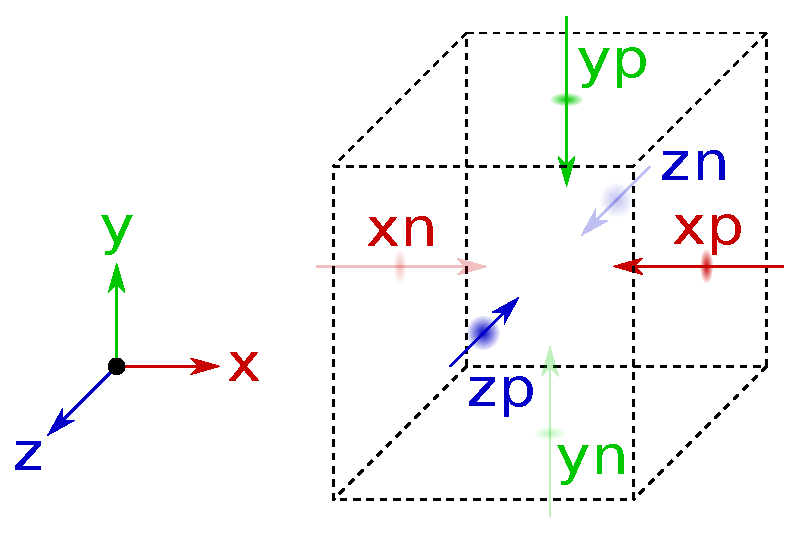
\includegraphics[width=0.4\linewidth]{3-Flow3DLabel}%
  \caption{Illustration of a region or subregion}%
  \label{fig:Flow3DLabel}
\end{figure}

In the implementation (\autoref{chap:Implementation}), subregions may be connected in multiple directions to form a \emph{\n{region}}.  A region is also a rectangular cuboid.  \autoref{fig:ModelHierarchy} shows the region and subregion within the model hierarchy.  However, this chapter only deals with one or two subregions at once.  Therefore, what will be called a subregion in the model implementation is often simply called a region in this chapter.

The subregion is the lowest level of spatial resolution, but it may contain multiple \emph{\n{species}} in multiple \emph{\np{phase}}.  Each of these \emph{\np{configuration}}, or species in certain phases, are treated as distinct but interacting entities.  The species and phases are also control volumes, but the model does not directly resolve the shape, location, and orientation of their boundaries.

Material, momentum, or energy may be \emph{transferred}\glsadd{transfer} among control volumes.  \emph{\N{material}} is synonymous with matter; it represents particles, atoms, or molecules.  Material is distinct from momentum and energy, although the transfer of material generally carries momentum and energy.  Since the model deals with chemical reactions and phase change, material is measured in terms of a number (which may be expressed in a unit such as the mole) rather than mass.  \N{material-adj} is also used as an adjective, as in material transfer.  \emph{\N{current}} is the flow rate of material, which may or may not be charged.  Electrical current is the flow rate of charge.  These and other key terms are listed in the glossary on page \pageref{mark:Glossary}.

There are two types of transfer.  \emph{Exchange} is transfer among different configurations within a subregion.  \emph{Transport} is transfer between similar configurations in neighboring subregions.  Thus, exchange is local and transport is spatial in nature.\footnote{Microscopically, exchange is also spatial, but the model is macroscopic.}  Chemical reactions and phases change involve material exchange---that is, transfer of matter among various configurations governed by the laws of chemistry.  Both types of transfer (exchange and transport) can generally occur by advection or diffusion.  These processes were introduced in \autoref{sec:DeclarativeLimitations} and will be discussed further in this chapter.

So far, two assumptions have been introduced: \begin{inparaenum}[(1)]\item all of the boundaries are rectangular and \item the subregions and regions have fixed boundaries\end{inparaenum}.  Further assumptions are introduced as necessary throughout the chapter.


It is important to note that the model equations are presented for a unit system where the gas and Faraday constants are normalized to one (see \autoref{sec:Units}).  This simplifies the equations and their implementation.  Also note that the \emph{\n{specific}} adjective is used to indicate ``per unit amount of material''.\footnote{In contrast, massic is defined by the \n{ISO} to mean ``per mass''~\cite{Taylor1995}.}  For example, specific mass is the mass per unit number of particles.  It is used instead of molar mass because the unit system is neutral with respect to the unit that represents the amount of material.  %A variable that represents the amount of material may be displayed in moles but the variable itself is not in moles (or any other unit of material).

\autoref{fig:AspectsOfFCModel} shows the high-level aspects that must be considered in a fuel cell model.  These will each be discussed in the following sections, with the exception of geometry (see above).  Many of the sections begin with a list of key features of the model that are either unusual or are new contributions.  The boxed equations are the ones that are actually implemented in the model (next chapter).  Other equations are presented to provide insight into the implemented equations and relate the model to established theories.

\begin{figure}[hbtp]
  \newcommand{\vgap}{\vphantom{Thermodynamic}}
\begin{tikzpicture}
    [level distance=1.75cm]
    \Tree[.FC\\Model
           [.{Material\\Properties}
             [.{Thermodynamic\vgap} ]
%                [.{Correlated\vgap} ]
%                [.{Derived\vgap} ] ]
             [.{Diffusion\vgap} ] ] 
           [.{Geometry\vgap} ]
           [.{Processes\vgap}
             [.\node[xshift=-0.98mm]{Exchange\vgap}; ]
             [.\node[xshift=-0.98mm]{Transport\vgap}; ]
             [.\node[xshift=-0.98mm]{Mixing\vgap}; ] ]
           [.{Conservation\vgap} ] ]
  \end{tikzpicture}
  \caption{Considerations of a fuel cell model}
  \label{fig:AspectsOfFCModel}
\end{figure}


\section{Correlated Thermodynamic Properties}
\label{sec:CorrelatedThermo}

\begin{contextbox}
  Highlights:
  \begin{itemize*}
    \item The correlations are necessary and sufficient to calculate basic thermodynamic properties (specific entropy, enthalpy, Gibbs energy, etc.) given temperature and pressure or specific volume.
    \item The correlations are polynomial and can be expanded as needed for accuracy.
    \item The pressure-volume-temperature correlation is sufficiently general to describe ideal gases, real gases, and incompressible species with or without thermal expansion.  Many fuel cell models are explicitly based on ideal gases under incompressible flow~\cite{Bernardi1991, Ceraolo2003, Karnik2007, Kim2010, Natarajan2001, Nguyen1993, Rubio2010, Sivertsen2005, Spiegel2008, Springer1991, Sunden2011, Um2000, Um2004, Wang2001, Wang2006, Weber2004, Yuan2010}.
    % Less pertinent:~\cite{Chen2004, Mangold2010, Pukrushpan2002, Serincan2011}
    \item The specific heat capacity-temperature correlation is general enough to model media with constant specific heat or to provide accurate information on the temperature dependence.  This makes it possible to simplify the descriptions of inert gases (e.g., \s{N2}) and more accurately describe reacting gases (\s{H2}, \s{H2O}, and \s{O2}) to model the temperature dependence of the cell potential.
  \end{itemize*}
\end{contextbox}
\vspace{0.7\baselineskip}


\subsection{Isobaric Specific Heat Capacity-Temperature Relation}

Isobaric specific heat capacity is defined by
\begin{equation}
  \label{eq:cpDefinition}
  \s{c}[_p] \equiv \s{T}\diffp{\s{s}}{\s{T}}[_p]
\end{equation}
where \s{s}~is specific entropy, \s{T}~is temperature, and \s{p}~is pressure.  McBride et al.\ provide the isobaric specific heat capacity of many species as a correlated polynomial of temperature~\cite{McBride2002}; however, \s{c}[_p]~is in general a function of both temperature and pressure.  For condensed species, they specify the thermodynamic state by the actual temperature and a reference pressure (\SI{1}{atm}).  The state of gases is chosen to be the ideal gas at the given temperature, since the specific heat capacity of an ideal gas is independent of pressure.  The correlation for this adjusted isobaric specific heat capacity is
\begin{equation}
  \label{eq:cpo}
  \s{c}[_p][^o] = \s{b}_1\s{T}^{-2} + \s{b}_2\s{T}^{-1} + \s{b}_3 + \s{b}_4\s{T} + \s{b}_5\s{T}^2 + \s{b}_6\s{T}^3 + \s{b}_7\s{T}^4
  \glsadd{_123}
\end{equation}
The coefficients ($\s{b}_1$, $\s{b}_2\glsadd{_123}$, \dots) must be chosen for the proper temperature range but are otherwise constant.  The model uses a more general form
\begin{equation}
  \boxed{\s{c}[_p][^o] = \sum_{\s{i} = 1}^{\s{m}}\s{b}[_i]\s{T}^{\s{i} + \s{n} - 1}}
\end{equation}
where \s{n}~is the power of the first term and the polynomial has an arbitrary number of terms~(\s{m}).  The order of the polynomial is $\s{m} + \s{n} - 1$.  Multiple sets of coefficients may be specified; they are selected depending on the temperature range (as per McBride et al.).


\subsection{Pressure-Volume-Temperature Relation}

The model uses the virial \n{EOS}, which was proposed by Thiesen in 1885 and validated against many gases by Kammerling-Onnes in 1901~\cite{Morrison1985, Nag2008}. %, \cite[p.~336]{Nag2008}.
It is convenient for use with differential equations and can be expanded as needed for accuracy.  The virial \n{EOS} can be expressed in a volume-explicit (or Leiden~\cite{McGlashan1973}) form as
\begin{equation}
  \label{eq:VirialLeiden1}%
  \s{v} = \s{b}_1\group{\frac{\s{p}}{\s{T}}}^{-1} + \s{b}_2 + \s{b}_3\group{\frac{\s{p}}{\s{T}}}^{1} + \s{b}_4\group{\frac{\s{p}}{\s{T}}}^{2} + \ldots
  \glsadd{_123}
\end{equation}
where the coefficients are functions of temperature only\cite{Dymond2002}. %[Eq.\ 1.3]
The model uses the following generalized form
\begin{equation}
  \label{eq:VirialLeiden}
  \boxed{\s{v} = \sum_{i = 1}^{\s{m}_1}\,\sum_{j = 1}^{\s{m}_2}\s{b}\sub{_i}[_j]\group{\frac{\s{p}}{\s{T}}}^{\s{i} + \s{n}_1 - 1}\s{T}^{\s{j} + \s{n}_2 - 1}}
  \glsadd{_123}
  \glsadd{_abc}
\end{equation}
where $\s{n}_1$ and $\s{n}_2$ are the powers of the first term and the polynomial has an arbitrary numbers of terms in both dimensions ($\s{m}_1$, $\s{m}_2$).  The $\s{p}/\s{T}$ group is used instead of~\s{p} so that \begin{inparaenum}[(1)]\item the matrix of coefficients ($\s{b}\sub{_i}[_j]$) is more compact for typical correlations (e.g.,~\cite{Dymond2002}) and \item the virial inverse matrix ($\s{b}\sub{_i}[_j]\sup{^prime}$ below) has the same size\end{inparaenum}.

The virial coefficients may be derived from the statistical mechanics of intermolecular forces~\cite{Salzman2004}.  For gases, the first virial coefficient ($\s{b}_1\glsadd{_123}$) is generally the gas constant, which has been normalized to one.  The second virial coefficient characterizes binary interactions between molecules---specifically the pair energy potential function~\cite{Dymond2002}.  The third coefficient is for ternary interactions, the fourth is for quaternary interactions, and so on~\cite{McGlashan1973}.  These effects diminish rapidly with the order of the interaction~\cite{Present1958}.  If $\s{b}_1 = 1\glsadd{_123}$ and the other terms are neglected, the virial \n{EOS} reduces to the ideal gas \n{EOS}.  For gases at low pressures, only the first and possibly the second virial coefficients are necessary.  Dymond et al.\ correlate the second virial coefficients of many gases to polynomials in temperature~\cite{Dymond2002}.

\autoref{eq:VirialLeiden1} is suitable for incompressible or even constant-volume species, where only the second virial coefficient ($\s{b}_2\glsadd{_123}$) is nonzero.  If the species is compressible, the volume-explicit form of \autoref{eq:VirialLeiden1} is equivalent to the following pressure-explicit (or Berlin) form~\cite{McGlashan1973, Dymond2002}:%\cite[Eq.\ 1.2]{Dymond2002}
\begin{equation}
  \label{eq:VirialBerlin1}%
  \frac{\s{p}}{\s{T}} = \s{b}_1^\prime\s{v}^{-1} + \s{b}_2^\prime\s{v}^{-2} + \s{b}_3^\prime\s{v}^{-3} + \s{b}_4^\prime\s{v}^{-4} + \ldots
  \glsadd{^prime}\glsadd{_123}
\end{equation}
Otherwise, pressure cannot be determined from temperature and specific volume.  The model uses the following generalized form:
\begin{equation}
  \label{eq:VirialBerlin}
  \boxed{\s{v} = \sum_{i = 1 - \s{m}_1}^{0}\,\sum_{j = 1}^{\s{m}_2}\s{b}\sub{_i}[_j]\sup{^prime}\s{p}^{\s{i} + \s{n}_1}\s{T}^{\s{j} + \s{n}_2}}
  \glsadd{_123}
  \glsadd{_abc}
\end{equation}
The modified coefficients of \autoref{eq:VirialBerlin1} are directly related to those of \autoref{eq:VirialLeiden1}~\cite{McGlashan1973, Dymond2002}:%\cite[Eqs.\ 1.4--1.6]{Dymond2002}
\begin{subequations}%
  \begin{empheq}[box=\fbox]{align}
    \s{b}_1^\prime &= \s{b}_1\\
    \s{b}_2^\prime &= \s{b}_2\\
    \s{b}_3^\prime &= \s{b}_2^2 + \s{b}_3\\
    \s{b}_4^\prime &= \s{b}_2^3 + 3\s{b}_2\s{b}_3 + \s{b}_4%\\
%                   &= \s{b}_2\group{\s{b}_2^2 + 3\s{b}_3} + \s{b}_4\tag*{}
%     \s{b}_5^\prime &= \s{b}_2^4 + 6\s{b}_2^2\s{b}_3 + 2\s{b}_3^2 + 4\s{b}_2\s{b}_4 + \s{b}_5\\
%                   &= \s{b}_2\group{\s{b}_2\group{\s{b}_2^2 + 6\s{b}_3} + 4\s{b}_4} + 2\s{b}_3^2 + \s{b}_5\tag*{}%
    \glsadd{^prime}\glsadd{_123}
  \end{empheq}
\end{subequations}%
We can determine the relations for even higher-order coefficients by setting Equations~\ref{eq:VirialLeiden1} and \ref{eq:VirialBerlin1} equal (in terms of $\s{p}\s{v}/\s{T}$) and successively eliminating terms~\cite{Salzman2004}.

% ``Virial coefficients Bi appear as coefficients in the virial expansion of the pressure of a many-particle system in powers of the density, providing systematic corrections to the ideal gas law.  They are characteristic of the interaction potential between the particles and in general depend on the temperature.  The second virial coefficient [Background.tex] depends only on the pair interaction between the particles, the third [Background.tex] depends on 2- and non-additive 3-body interactions, and so on.'' [Wikipedia]

% ``Unlike empirical equations of state, such as the van der Waals equation (which is, at best, very approximate) and the Beattie-Bridgeman equation (which is now rarely used) which are discussed in GNS, the virial equation can be derived from exact statistical mechanical theory.'' [\url{http://voh.chem.ucla.edu/vohtar/spring06/classes/114/pdf/T9-Joule-Thomson%20Coefficient}]
% Originally from one of the following?
%   H. Kamerlingh Onnes (1901)
%   J. O. Hirschfelder, C. F. Curtiss, and R. B. Bird, Molecular Theory of Gases and Liquids, Wiley, New York, (1954)
%   W. J. Moore, Physical Chemistry, 4th ed., Prentice-Hall, Englewood Cliffs, N.J. (1972), pp.26, 130, 926.

% Also:  \cite[p. 379]{Brown2000}


\section{Derived Thermodynamic Properties}
\label{sec:DerivedThermo}

\begin{contextbox}
  Highlights:
  \begin{itemize*}
    \item The derivations are exact and do not involve additional assumptions besides those inherent in the correlated properties of \autoref{sec:CorrelatedThermo}.
    \item The properties are general and complete enough that the model does not require specialized thermodynamic correlations such as the saturation pressure-temperature curve of \n{H2O}.
  \end{itemize*}
\end{contextbox}
\vspace{0.7\baselineskip}

% \cite[pp.~16--18]{Dymond2002} provides equations for adjustment of properties from ideal gas, but they may be incorrect.


\subsection{Specific Entropy}
  \label{sec:SpecificEntropy}

We can write specific entropy as
\begin{equation}
  \s{s} = \int_0^{\s{T}}\frac{\s{c}[_p][^o]}{\s{T}}\,\mathrm{d}\s{T} + \int_{\s{p}[^o]}^{\s{p}}\diffp{\s{s}}{\s{p}}[_T]\mathrm{d}\s{p}%
\end{equation}
where $\s{c}[_p][^o]$ is evaluated at reference pressure $\s{p}[^o]$.  Applying the appropriate Maxwell relation, $(\partial\s{s}/\partial\s{p})_T = -(\partial\s{v}/\partial\s{T})_p$, this is
\begin{equation}
  \label{eq:s}
  \boxed{\s{s} = \int_0^{\s{T}}\frac{\s{c}[_p][^o]}{\s{T}}\,\mathrm{d}\s{T} - \int_{\s{p}[^o]}^{\s{p}}\diffp{\s{v}}{\s{T}}[_p]\mathrm{d}\s{p}}%
\end{equation}
which can be evaluated using Equations~\ref{eq:cpo} and \ref{eq:VirialLeiden1}.  McBride et al.~\cite{McBride2002} give the integration constant of the first term for each species so that the isobaric specific heat correlation does not need to be evaluated at (or even valid at) absolute zero temperature.  The second integral is $\ln{(\s{p}/\s{p}[^o])}$ for an ideal gas and typically small for condensed species.  Again, the second- and higher-order virial coefficients ($\s{b}_2$, $\s{b}_3\glsadd{_123}$, \dots) are functions of temperature but not pressure.  The coefficients of isobaric specific heat capacity ($\s{b}_1$, $\s{b}_2\glsadd{_123}$, \dots) may be treated as constant but must be chosen based on the temperature range.

For gases, the lower limit of the second integral of \autoref{eq:s} is evaluated only for the first virial coefficient.  This adjustment is necessary because the reference for the \s{c}[_p]-\s{T} correlation is the ideal gas instead of the real gas.  Formally, the modified form of \autoref{eq:s} for gases is
\begin{equation}
  \label{eq:sGas}
  \s{s} = \int_0^{\s{T}}\frac{\s{c}[_p][^o]}{\s{T}}\,\mathrm{d}\s{T} - \Group{\int_{\s{p}[^o]}^0\diffp{\s{v}[_IG]}{\s{T}}[_p]\mathrm{d}\s{p} + \int_0^{\s{p}}\diffp{\s{v}}{\s{T}}[_p]\mathrm{d}\s{p}}%
\end{equation}
where the first integral in square brackets involves the specific volume of the ideal gas and the second involves the real gas.  Following the approach by Rao~\cite{Rao1997}, %[p.~271]
the ideal gas contribution is integrated from the reference pressure to zero pressure and the real gas contribution is integrated from zero pressure to the actual pressure.  At zero pressure, binary and higher-order molecular interactions are eliminated and a real gas behaves as an ideal gas.

\autoref{fig:IntegrationPath} depicts the integration path of the pressure terms.  Assuming that the first virial coefficient ($\s{b}_1\glsadd{_123}$) is the same for the ideal gas and the real gas (since for gases $\s{b}_1 = 1\glsadd{_123}$), the contribution of the first-order virial term may be integrated directly from \s{p}[^o] to~\s{p}.  In effect, this combines $\ln{(0/\s{p}[^o])} + \ln{(\s{p}/0)}$ to give $\ln{(\s{p}/\s{p}[^o])}$.  Since the contributions of the second- and higher-order virial coefficients are zero at zero pressure, we can eliminate those integral evaluations.  The net result is that the lower limit of the second integral in \autoref{eq:s} is evaluated for the ideal gas and the upper limit is evaluated for the real gas.

\begin{figure}[htbp]
  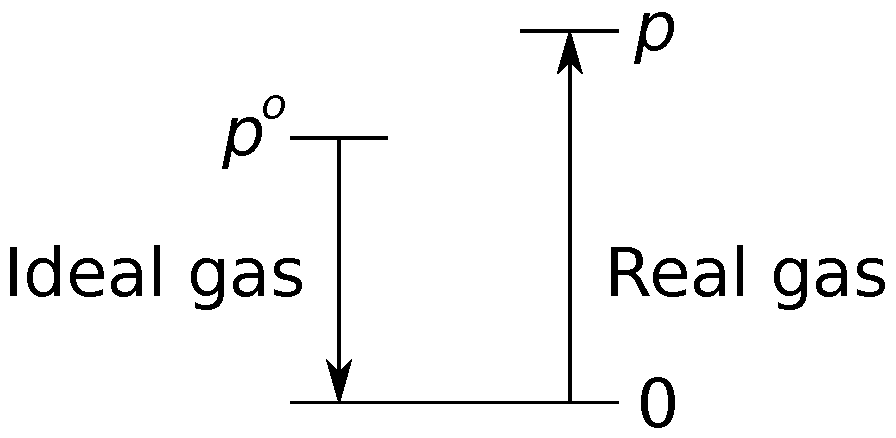
\includegraphics[width=0.3\linewidth]{3-IntegrationPath}%
  \caption{Integration path for the specific entropy of gases}%
  \label{fig:IntegrationPath}
\end{figure}

\subsection{Specific Enthalpy}

We can define specific enthalpy by the differential equation
\begin{equation}
  \label{eq:dh}%
  \mathrm{d}\s{h} = \s{T}\mathrm{d}\s{s} + \s{v}\mathrm{d}\s{p}
\end{equation}
After substituting \autoref{eq:s} and integrating with an adjustable temperature reference, this is
\begin{equation}
  \label{eq:h}%
  \boxed{\s{h} = \int_{\s{T}[^o]}^{\s{T}}\s{c}[_p][^o]\,\mathrm{d}\s{T} + \int_{\s{p}[^o]}^{\s{p}}\Group{\s{v} - \s{T}\diffp{\s{v}}{\s{T}}[_p]}\mathrm{d}\s{p}}%
\end{equation}
which can be evaluated using Equations~\ref{eq:cpo} and \ref{eq:VirialLeiden1}.  As for specific entropy, if the species is a gas, the lower limit of the second integral is of the ideal gas and the upper limit is of the real gas.  The second integral is zero for an ideal gas and typically small for condensed species.  McBride et al.~\cite{McBride2002} give the sufficient integration constants and offsets to specify the enthalpy reference such that \begin{inparaenum}[(1)]
  \item the enthalpy at \SI{0}{K} and \s{p}[^o]~is zero,
  \item the enthalpy at \SI{25}{\celsius} and \s{p}[^o]~is zero, or
  \item the enthalpy at \SI{25}{\celsius} and \s{p}[^o]~is the enthalpy of formation at that temperature and pressure.
\end{inparaenum}


\subsection{Specific Gibbs Energy}

We can define specific Gibbs energy by the following differential equation:
\begin{equation}
  \label{eq:GibbsFunction}
  \mathrm{d}\s{g} = \s{v}\mathrm{d}\s{p} - \s{s}\mathrm{d}\s{T}
\end{equation}
In conjunction with \autoref{eq:dh}, this implies that
\begin{equation}
  \label{eq:g}
  \s{g} = \s{h} - \s{T}\s{s}
\end{equation}
Substituting Equations~\ref{eq:s} and \ref{eq:h},
\begin{equation}
  \label{eq:gExpanded}
  \boxed{\s{g} = \int_{\s{p}[^o]}^{\s{p}}\s{v}\,\mathrm{d}\s{p} + \s{T}\int_{\s{p}[^o]}^{\s{p}}\diffp{\s{v}}{\s{T}}[_p]\mathrm{d}\s{p} - \int_{\s{p}[^o]}^{\s{p}}\s{T}\diffp{\s{v}}{\s{T}}[_p]\mathrm{d}\s{p} + \int_{\s{T}[^o]}^{\s{T}}\s{c}[_p][^o]\,\mathrm{d}\s{T} - \s{T}\int_0^{\s{T}}\frac{\s{c}[_p][^o]}{\s{T}}\,\mathrm{d}\s{T}}%
\end{equation}
which can be evaluated using Equations~\ref{eq:cpo}, \ref{eq:VirialLeiden1}, and \ref{eq:VirialBerlin1}.  If the species is a gas, the lower limits of the pressure integrals are of the ideal gas and the upper limits are of the real gas (see \autoref{sec:SpecificEntropy}).

% Electrochemical free potential of species is the sum of Gibbs potential and electric work potential \cite[Equation~3.16, p.~82]{Newman1991}:
% \begin{equation}
%   \s{mu}[_i] = \s{mu}[_i]^{chem} + \s{z}[_i]\s{Phi}
% \end{equation}
% Electrical work potential is the work required to bring the particles together from infinite distance slowly (i.e., electrostatic) [\url{http://en.wikipedia.org/wiki/Electric_potential_energy}].

% Discussion of conflicting names for chemical and electrochemical potential: \url{http://www.tf.uni-kiel.de/matwis/amat/def_en/kap_2/advanced/t2_4_1.html}


\subsection{Isobaric Specific Heat Capacity}

We can express the isobaric specific heat capacity by substituting \autoref{eq:s} into \autoref{eq:cpDefinition}.
\begin{equation}
  \label{eq:cp}
  \boxed{\s{c}[_p] = \s{c}[_p][^o] - \s{T}\diffp{\Group{\int_{\s{p}[^o]}^{\s{p}}\diffp{\s{v}}{\s{T}}[_p]\mathrm{d}\s{p}}}{\s{T}}[_p]}%
\end{equation}
This can also be evaluated using Equations~\ref{eq:cpo} and \ref{eq:VirialLeiden1}.  The second term is zero for an ideal gas and usually small for condensed species.  If the species is a gas, the lower limit of the integral is of the ideal gas and the upper limit is of the real gas (see \autoref{sec:SpecificEntropy}).


\subsection{Isochoric Specific Heat Capacity}

Isochoric specific heat capacity is defined by
\begin{equation}
  \label{eq:cvDefinition}
  \s{c}[_v] \equiv \s{T}\diffp{\s{s}}{\s{T}}[_v]
\end{equation}
The isochoric and isobaric specific heat capacities are related by the following equation~\cite{Moran2004}: %[p.~546]
\begin{equation}
  \boxed{\s{c}[_v] = \s{c}[_p] - \s{T}\diffp{\s{p}}{\s{T}}[_v]\diffp{\s{v}}{\s{T}}[_p]}
\end{equation}
Applying \autoref{eq:cp}, this is
\begin{equation}
  \s{c}[_v] = \s{c}[_p][^o]- \s{T}\Group{\diffp{\s{p}}{\s{T}}[_v]\diffp{\s{v}}{\s{T}}[_p] + \diffp{\Group{\int_{\s{p}[^o]}^{\s{p}}\diffp{\s{v}}{\s{T}}[_p]\mathrm{d}\s{p}}}{\s{T}}[_p]}%
\end{equation}
which can be evaluated using Equations~\ref{eq:cpo}, \ref{eq:VirialLeiden1}, and \ref{eq:VirialBerlin1}.  It reduces to $\s{c}[_v] = \s{c}[_p] - 1$ for an ideal gas.  If the species is a gas, the lower limit of the integral is of the ideal gas and the upper limit is of the real gas (see \autoref{sec:SpecificEntropy}).


\section{Mixtures}
\label{sec:Mixtures}

\begin{contextbox}
  Highlights:
  \begin{itemize*}
    \item Traditionally, Dalton's and Amagat's laws are used with the ideal gas assumption, but the model does not impose that requirement.\footnote{This is an approximation.  The alternative would to formulate another, more detailed p-v-T relation that encompasses the entire mixture---possibly as a correction pressure or volume.  That is beyond the present scope.}
    \item The volumes and pressures of mixtures can change dynamically, but the model imposes Dalton's and Amagat's laws exactly and instantaneously.  %For example, the volumes of the phases always add to the total volume of the region.
    There are no additional states.
  \end{itemize*}
\end{contextbox}
\vspace{0.7\baselineskip}

% \begin{figure}[!htb]
%   \newcommand{\vgap}{\vphantom{Mixing}}
%   \centering
%   \begin{tikzpicture}
%     [level distance=1.5cm,
%      level 2/.style={level distance=1.1cm}]
%     \Tree[.FC\\Model
%            [.{Processes\vgap}
%               [.{Mixing\vgap}
%                 [.{Additivity\\of Pressure} ]
%                 [.{Additivity\\of Volume} ] ] ] ]
%   \end{tikzpicture}
%   \caption{Types of mixing regimes in the fuel cell model}
% \end{figure}

% Departures from Dalton's and Amagat's laws:~\cite{Din1965}

% \cite{Woo1995}:
% ``The significance of the preceding derivation is that, in a mixture of gases (black and white), Dalton's law calculates the properties of a gas (black) assuming the other gas (white) is not there, whereas Amagat's law calculates the properties of the black molecules assuming that the white molecules are there and interact with the black just as do other black molecules.  Put another way, the ideal gas law assumes that molecules are blind, they `see' no other molecules; Dalton's law assumes that the molecules are selectively blind, they see only molecules of their own `color'; Amagat's law assumes that the molecules are colorblind, they `see' all molecules but think they are the same color.''

% Gibbs-Dalton law is an extension of Dalton's law of additive pressures applied to an ideal gas \url{http://www.scribd.com/doc/27396916/187/Gibbs-Dalton-law}.

% Amagat's law is analogous to the serial connection of many particles (pressures equal at a point, length is additive) and Dalton's law is analogous to the parallel connection of many particles (each species is a branch; lengths equal, pressures additive).


\subsection{Species within a Phase}
\label{sec:DaltonsLaw}

The model combines species within a phase using Dalton's law of partial pressures, which states that the partial pressures of the components of a mixture add to the total pressure of the mixture~\cite{Bejan2006}:%[p.~192]
\begin{equation}
  \boxed{\s{p} = \sum\s{p}[_i]}
\end{equation}
Dalton's law also states that each species~\s{i} exists at the total volume of the phase:
\begin{equation}
  \boxed{\s{V}[_i] = \s{V}}
\end{equation}
For example, according to this concept, the atmospheric gases of~\s{N2}, \s{O2}, etc.\ each occupy the total volume of the air but only contribute partially to the pressure of the air.


\subsection{Phases within a Region}
\label{sec:AmagatsLaw}

The model combines phases within a region using Amagat's law of partial volumes, which states that the partial extensive volumes of the components of a mixture sum to the total extensive volume of the mixture~\cite{Bejan2006}:%[p.~194]
\begin{equation}
  \boxed{\s{V} = \sum\s{V}[_i]}
\end{equation}
In the model, \s{V}[_i]~is the volume of a phase and \s{V}~is the volume of the region, which is fixed.  Amagat's law also states that each species~\s{i} exists at the total pressure of the phase:
\begin{equation}
  \boxed{\s{p}[_i] = \s{p}}
\end{equation}

The model only uses Amagat's law for distinct phases within a region---not for species within a phase.  Amagat's law loses its physical meaning as species are mixed~\cite{Woo1995}.  If species are fully mixed, it is impossible to distinguish the particles and thus determine the partial volumes.

For example, if a system contains a solid phase and air, the model states that the solid and the air experience the same pressure and occupy only part of the total volume (Amagat's law).  Within the air, the gases mix according to Dalton's law (\autoref{sec:DaltonsLaw}).  The model applies Dalton's law and Amagat's law dynamically, which makes it possible to describe the formation of liquid water in the cell~\cite{Bevers1997, Li2005, Weber2004ChemRev}.

The model is classified as a Euler-Euler approach rather than a Euler-Lagrange approach~\cite{Fluent6.3}, since all phases are tracked from a Eulerian perspective.  The volume fractions are continuous functions of time and must sum to one.  The Euler-Lagrange approach is limited to problems where the solid phase has a small volume in comparison to the fluid phase---10\% to 12\%~\cite{Fluent6.3}.  This is not appropriate for the layers of a fuel cell.


\section{Basic Conservation Equations}
\label{sec:BasicConservation}

\begin{contextbox}
  Highlights:
  \begin{itemize*}
    \item The model is dynamic.  It includes material, momentum, and energy storage.
    \item Each species has its own conservation equations for material, translational momentum, and energy.  However, the model's parameters can be set so that the translation tool combines certain conservation equations through index reduction.  The concept of separate momentum balances for each species is unusual but not unprecedented in the literature~\cite{Wesselingh2000, Kerkhof2005AIChE, Kerkhof2005ChemEngSci}.  Separate energy balances are rarely used (\cite{Kuropatenko2005} is one example).
  \end{itemize*}
\end{contextbox}
\vspace{0.7\baselineskip}

Material, momentum, and energy are conserved throughout the model at interfaces and within regions.  Each configuration (i.e., each species in each phase) has its own conservation equation in every region.  The conserved quantities can be stored in configurations but not at interfaces between or among configurations.

Below, the conservation equations (i.e., balances) are introduced with minimal detail to explain the exchange and transport equations (Sections~\ref{sec:Exchange} and \ref{sec:Transport}).  The interfaces are generalized here, but there are two types:  boundaries between regions (for transport) and transitions among configurations within a region (for exchange).  In general, the flow through each interface has advective and diffusive components.  Later, in \autoref{sec:DetailedConservation}, detailed conservation equations will be presented.


\subsection{Material}
\label{sec:BasicMaterialBalance}


The rate of storage of material is equal to the net rate of intake or transfer of material into a control volume.  \autoref{fig:MaterialIntake} shows that there are two types of material transfer---exchange and transport.  In general, exchange and transport can each occur by advection or diffusion.  However, the model considers chemical reactions and phase change, the two modes of material exchange, to be diffusive processes.

\begin{figure}[hbtp]
  \newcommand{\vgap}{\vphantom{Body}}
  \begin{tikzpicture}
    [level distance=1.75cm]
    \Tree[.{Material\\transfer}
           [.{Transport\vgap}
             [.{Advective\vgap} ]
             [.{Diffusive\vgap} ] ]
           [.{Exchange\vgap}
             [.{Diffusive\vgap}
               [.{Chemical\\(reaction)\vgap} ]
               [.{Physical\\(phase change)\vgap} ] ] ] ]
  \end{tikzpicture}
  \caption{Types of material intake considered in the model}
  \label{fig:MaterialIntake}
\end{figure}


For now, the material balance will be written simply as
\begin{equation}
  \newcommand{\vgap}{\vphantom{\diffp{\s{N}}{\s{t}}}}
  \label{eq:MaterialBalance}%
  \boxed{\underbrace{\vgap\diffp{\s{N}}{\s{t}}}_\text{storage} =  \,\, \underbrace{\vgap\sum\dot{N}[_i]}_\text{intake}}
\end{equation}
where \s{N}~is the particle number or amount of material and \dot{N}[_i] is the total current (advective and diffusive, $\dot{N}\sub{_A}[_i] + \dot{N}\sub{_D}[_i]$) into a generalized interface~\s{i}.  The use of a partial derivative ($\diffp{\s{N}}{\s{t}}$) rather than a total derivative ($\frac{\mathrm{d}\s{N}}{\mathrm{d}\s{t}}$) serves as a reminder that the model is Eulerian.  Although the equation is written in terms of material, mass is conserved as well since the specific mass of each configuration is constant and the phase change and reaction processes are balanced in terms of mass.

At boundaries and transitions, there is no material storage.  Advection has no net effect because the rate of advection is continuous across a boundary.  Therefore, the material balance reduces to
\begin{equation}
  \label{eq:MaterialBalanceInterface}
  \boxed{0 = \sum\dot{N}\sub{_D}[_i]}
\end{equation}
where the summation is now across all interacting configurations~\s{i}.  This equation is generated automatically by the connection equations of the \n{EOO} language; it is the generalized Kirchhoff current law for material.


\subsection{Rotational Momentum}
\label{sec:RotationalConservation}

The model is based on the assumption that rotational momentum is not stored.  Rotational momentum is not exchanged or transported axially through boundaries, but it is conveyed through shear forces.  We assume that the forces are point forces in the center of the boundaries and that the axes of rotation are centered in the region.  Therefore,
\begin{subequations}
  \label{eq:RotationalConservation}
  \begin{empheq}[box=\fbox]{align}
    0 &= \group{\dot{mPhi}\sub{_z}[_neg][_y] - \dot{mPhi}\sub{_z}[_pos][_y]}\s{L}[_z] - \group{\dot{mPhi}\sub{_y}[_neg][_z] - \dot{mPhi}\sub{_y}[_pos][_z]}\s{L}[_y] \label{eq:RotationalConservationX} \\
    0 &= \group{\dot{mPhi}\sub{_x}[_neg][_z] - \dot{mPhi}\sub{_x}[_pos][_z]}\s{L}[_x] - \group{\dot{mPhi}\sub{_z}[_neg][_x] - \dot{mPhi}\sub{_z}[_pos][_x]}\s{L}[_z] \label{eq:RotationalConservationY} \\
    0 &= \group{\dot{mPhi}\sub{_y}[_neg][_x] - \dot{mPhi}\sub{_y}[_pos][_x]}\s{L}[_y] - \group{\dot{mPhi}\sub{_x}[_neg][_y] - \dot{mPhi}\sub{_x}[_pos][_y]}\s{L}[_x] \label{eq:RotationalConservationZ}
  \end{empheq}
\end{subequations}
where $\dot{mPhi}\sub{_z}[_neg][_y]$ is the force in the y-direction through the negative-z boundary, $\dot{mPhi}\sub{_y}[_pos][_z]$ is the force in the z direction through the positive-y boundary, and so on.  The normal forces do not introduce torque since they are aligned with the center of rotation.  These equations are included in the diffusion equations for shear force around each axis (\autoref{sec:TransverseTransport}).


\subsection{Translational Momentum}
\label{sec:BasicTranslationalBalance}


The rate of storage of translational momentum is equal to the sum of the forces on a control volume.  As shown by \autoref{fig:MaterialIntake}, there are three types of forces on a configuration within a region: body forces, surface forces, and intermolecular forces.  The body forces may be gravitational or electric; magnetic and nuclear forces are assumed to be negligible.  The surface forces include the effects of thermodynamic pressure, advection (i.e., dynamic pressure), and diffusion (i.e., nonequilibrium pressure~\cite{Meier2005} and shear stress).  The thermodynamic pressure is always normal to the surface, but advection and diffusion also have transverse components.  The intermolecular or exchange forces may be advective or diffusive.  Advective exchange occurs, for example, in a reacting stream where the reactants are traveling relative to the control volume.  Diffusive exchange occurs in multi-component fluids when the species are traveling at different velocities.

\begin{figure}[hbtp]
  \newcommand{\vgap}{\vphantom{Body}}
  \begin{tikzpicture}
    [level distance=1.75cm]
    \Tree[.\node[xshift=-0.3mm]{Forces\vgap};
           [.{Body\vgap}
             [.{Gravi-\\tational} ]
             [.{Electric\vgap} ] ]
           [.{Transport\\(surface)}
             [.{Pressure\vgap}
               [.{Thermo-\\dynamic} ]
               [.{Advective\\(dynamic)}
                 [.{Normal\vgap} ]
                 [.{Transverse\vgap} ] ] ]
             [.{Diffusive\\(viscous)}
                 [.{Normal\\(bulk)\vgap} ]
                 [.{Transverse\\(shear)} ] ] ]
           [.{Exchange\\(intermolecular)}
             [.{Advective\vgap} ]
             [.{Diffusive\vgap} ] ] ]
  \end{tikzpicture}
  \caption{Types of forces considered in the model}
  \label{fig:Forces}
\end{figure}


For now, we will generalize the advective and diffusive forces to encompass both exchange and transport.  We will also combine the normal and transverse components of transport.  Therefore, the translational momentum balance can be written as
\begin{equation}
  \newcommand{\vgap}{\vphantom{\diffp{\group{\s{M}\s{phi}}}{\s{t}}}}%
  \label{eq:TranslationalBalance}%
  \underbrace{\diffp{\group{\s{M}\s{phi}}}{\s{t}}}_\text{storage} + \underbrace{\vgap\s{M}\s{a} + \s{Z}\s{E}}_\text{body} + \underbrace{\vgap\s{A}\Delta\s{p}[_i]}_{\substack{\text{thermo-}\\\text{dynamic}}} = \sum\Big(\underbrace{\vgap\s{m}\s{phi}[_i]\dot{N}[_i]}_\text{advection} + \underbrace{\vgap\dot{mPhi}\sub{_D}[_i]}_\text{diffusion}\Big)
\end{equation}
where \s{phi}~is a component of velocity, \s{E}~is the electric field, and \s{a}~represents the acceleration due to additional body forces.  The mass \s{M}~is $\s{m}\s{N}$ and the charge \s{Z}~is $\s{z}\n{N}$, where \s{m}~is the specific mass, \s{z}~is the charge number, and \s{N}~is the amount of material known from the state of the material balance~(\ref{eq:MaterialBalance}).  The diffusive terms (\dot{mPhi}[_D]) include shear forces, nonequilibrium normal forces, and drag among configurations.

The advective forces ($\s{m}\s{phi}\dot{N}$) account for convective acceleration and the momentum transferred in reacting flows and phase change.  It is important to note again that the material transfer (\dot{N}) includes both advection and diffusion.  Momentum is advected or carried by material regardless of whether that material is transferred by advection or diffusion.

The difference ($\Delta$) on the left side of \autoref{eq:TranslationalBalance} is across the boundaries normal to the component of translational momentum.  The variable~\s{A} is the area of those boundaries.  The thermodynamic force term ($\s{A}\Delta\s{p}[_i]$) is based on the assumption that the configuration experiences pressure across the entire cross-sectional area of the region, although in reality the area is reduced if other phases are present.  This is necessary to ensure that translational momentum is conserved between two adjacent regions.


At boundaries and transitions, there is no storage.  The advective terms of \autoref{eq:TranslationalBalance} cancel because the advected properties are continuous at the interface.  The thermodynamic pressure is continuous at the interface and thus has no effect.  There is no material in the interface, so there are no body forces.  Therefore, the conservation of translational momentum reduces to
\begin{equation}
  \label{eq:TranslationalBalanceInterface}
  \boxed{0 = \sum\dot{mPhi}\sub{_D}[_i]}
\end{equation}
where the summation is now across all interacting configurations~\s{i}.  This equation is generated automatically by the connection equations of the \n{EOO} language; it is the generalized Kirchhoff current law for translational momentum.


\subsection{Energy}
\label{sec:BasicEnergyBalance}


The rate of storage of energy in a control volume is equal to the net rate of intake.  As shown in \autoref{fig:EnergyIntake}, the intake can be divided into material, translational, and thermal parts.  Although not shown, each of these forms may be transferred by exchange or transport.  The translational and thermal energy transfers can be due to advection or diffusion.  The material transfer of energy is not labeled as advective or diffusive in \autoref{fig:EnergyIntake} because it requires further explanation.  The material itself can be transferred by advection or diffusion, but the associated energy transfer is purely advective because the energy is carried by material.

\begin{figure}[hbtp]
  \newcommand{\vgap}{\vphantom{($\frac{1}{2}\s{m}\s{phi}^2$)}}
  \begin{tikzpicture}
    [level distance=1.75cm]
    \Tree[.\node[xshift=-5.7mm]{Energy\\intake};
            [.{Material\\(\s{g})\vgap} ]
            [.{Translational\vgap}
              [.{Advective\\($\frac{1}{2}\s{m}\s{phi}^2$)\vgap} ]
              [.{Diffusive\\(viscous)\vgap} ] ]
            [.{Thermal\vgap}
              [.{Advective\\(\s{T}\s{s})\vgap} ]
              [.{Diffusive\\(conduction)\vgap} ] ] ]
  \end{tikzpicture}
  \caption{Types of energy intake considered in the model}
  \label{fig:EnergyIntake}
\end{figure}

Thermal conduction is synonymous with thermal diffusion.  Thermal convection is the combined effect of diffusive thermal exchange between phases (often a solid and a fluid) and the subsequent transport of thermal energy via advection of the fluid.  The thermal advection factor ($\s{T}\s{s}$) and the material factor~(\s{g}) constitute specific enthalpy ($\s{h} = \s{g} + \s{T}\s{s}$, \autoref{eq:g}).  Combined with the translational advection factor, this is specific enthalpy plus specific kinetic energy ($\s{h} + \frac{1}{2}\s{m}\s{phi}^2$).


The factors of \autoref{fig:EnergyIntake} are incorporated into the right side of the energy balance equation:
\begin{equation}
  \newcommand{\vgap}{\vphantom{\frac{\s{m}\s{phi}[_i]^2}{2}\dot{N}[_i] + \s{phi}[_i]\dot{mPhi}\sub{_D}[_i]}}
  \label{eq:EnergyBalance}
  \underbrace{\underbrace{\vgap\s{g}\diffp{\s{N}}{\s{t}}}_\text{material} \, + \underbrace{\vgap\frac{\partial\group{\s{M}\s{phi}^2}}{2\partial\s{t}}}_\text{translational} + \,\, \underbrace{\vgap\s{T}\diffp{\s{S}}{\s{t}}}_\text{thermal}}_\text{storage} \,\, = \,\, \underbrace{\sum\Big[\underbrace{\vgap\s{g}[_i]\dot{N}[_i]}_\text{material} + \underbrace{\s{phi}[_i]\Big(\underbrace{\vgap\frac{\s{m}\s{phi}[_i]}{2}\dot{N}[_i]}_\text{advection} + \underbrace{\vgap\dot{mPhi}\sub{_D}[_i]}_\text{diffusion}\Big)}_\text{translational} + \underbrace{\vgap\underbrace{\vgap\group{\s{T}\s{s}}[_i]\dot{N}[_i]}_\text{advection} + \underbrace{\vgap\dot{Q}\sub{_D}[_i]}_\text{diffusion}}_\text{thermal}\Big]}_\text{intake}
\end{equation}
where \dot{N}[_i] is the total current (advective and diffusive) into interface~\s{i}.  This equation applies to every species in every phase.  It has been assumed that the control volume is stationary with respect to external fields (e.g., no gravitational work), although the fluid may move against those fields within the control volume.   The translational diffusion term, in conjunction with the translational (or kinetic) storage term, accounts for viscous dissipation.  This will be more apparent in later forms of the energy balance (e.g.,~\autoref{eq:EnergyBalanceIntensive2}).

The material and thermal storage terms ($\s{g}\diffp{\s{N}}{\s{t}} + \s{T}\diffp{\s{S}}{\s{t}}$) are equivalent to $\diffp{\s{H}}{\s{t}} - \s{V}\diffp{\s{p}}{\s{t}}$ or $\diffp{\s{U}}{\s{t}} + \s{p}\diffp{\s{V}}{\s{t}}$, where $\s{p}\diffp{\s{V}}{\s{t}}$ is the boundary work done by the configuration.\footnote{The form of \autoref{eq:EnergyBalance} has been chosen so that the material, translational, and thermal terms are explicit on both sides.  Specific flow work (\s{p}\s{v}) is considered a part of the material term.}  The boundary work can only be due to expansion of the phases in which the configuration belongs (and contraction of other phases) because the volume of the region is fixed.  The translational storage term describes the change in macroscopic kinetic energy.


At boundaries and transitions, there is no energy storage.  The advective terms cancel because the advected properties are continuous at the interface.  The translational diffusion terms can be removed because they sum to zero according to \autoref{eq:TranslationalBalanceInterface}.  Therefore, the conservation of energy reduces to
\begin{equation}
  \label{eq:ThermalBalanceInterface}
  \boxed{0 = \sum\dot{Q}\sub{_D}[_i]}
\end{equation}

where the summation is now across all interacting configurations~\s{i}.  This equation is generated automatically by the connection equations of the \n{EOO} language; it is the generalized Kirchhoff current law for heat transfer.


\section{Exchange Equations}
\label{sec:Exchange}

\begin{contextbox}%
  Highlights:
  \begin{itemize*}
    \item A common modeling framework is used for phase change, intermolecular drag, and intermolecular thermal conduction.
    \item The transfer of translational momentum and energy due to phase change and reactions is described as pure advection.
    \item An analogy is established between the total (advective plus diffusive) rate of exchange and the material derivative.
    \item The model describes phase change dynamically.  It does not assume instantaneous phase equilibrium in the sense of the Gibbs phase rule~\cite{Moran2004, Bejan2006}.  This avoids nonlinear systems of equations while using the previously established properties (i.e., no need to establish a separate correlation for saturation pressure).
    \item The rate of phase change is proportional to the difference in chemical activity between the phases.
    \item A property called independity is defined which generalizes the concept of mobility for translational interactions to thermal interactions.
  \end{itemize*}
\end{contextbox}

% \begin{figure}[!htb]
%   \newcommand{\vgap}{\vphantom{Exchange}}
%   \centering
%   \begin{tikzpicture}
%     [level distance=1.5cm,
%      level 2/.style={level distance=1.1cm}]
%     \Tree[.FC\\Model
%            [.{Processes\vgap}
%               [.{Exchange\vgap}
%                 [.{Advection\vgap} ]
%                 [.{Diffusion\vgap} ] ] ] ]
%   \end{tikzpicture}
%   \caption{Types of exchange processes in the fuel cell model}
% \end{figure}

\emph{\N{exchange}} is the transfer of a conserved quantity---material, momentum, or energy---among different configurations of material that exist within a region.  In general, it is due to advection and diffusion.  Advective exchange is the transfer of the quantity along with a sustained transfer of material between species (i.e., reaction) or different phases of a single species (i.e., phase change).  Diffusive exchange is the transfer of the quantity due only to collisions or thermal agitation of the particles, without a sustained material transfer.  In diffusion, a particle leaves one configuration (i.e., a species in a certain phase) with the specific quantity (or particle-average amount of the quantity) within the configuration and returns with the specific quantity of the other configuration.  This brings certain intensive properties---specific Gibbs energy, velocity, and temperature---into equilibrium among the configurations.


The model of exchange is based on the assumption that advection and diffusion are independent yet additive.  The total rate of exchange of the quantity~\s{X} into a configuration~\s{j} due to interaction or transition~\s{i} is the sum of the advective and diffusive rates:
\begin{equation}
  \label{eq:Exchange}
  \dot{X}\sub{_i}[_j] = \dot{X}\sub{_A}[ ][_i][_j] + \dot{X}\sub{_D}[ ][_i][_j]
\end{equation}
For material exchange, the quantity~(\s{X}) is the amount of material~(\s{N}).   For translational exchange, it is the product of the amount of material and velocity~(\s{Phi}).  For thermal exchange, it is heat~(\s{Q}).  The phase change and reaction processes are purely advective in terms of translational momentum and energy.  Particles from the source (e.g., reactants) carry properties through the process without intermediately mixing with particles from the sink (e.g., products).  Meanwhile, there are diffusive interactions for translational momentum and energy that are independent of the phase change and reactions.



\noindent\underline{\textbf{Advection}}

The rate of advective exchange is the product of the current and the amount of the exchanged quantity carried by the material.
\begin{equation}
  \label{eq:AdvectiveExchange1}
  \dot{X}\sub{_A}[ ][_i][_j] = \dot{N}\sub{_i}[_j]\diffp{\s{X}}{\s{N}}[_i][_j]
\end{equation}
The variable $\dot{N}\sub{_i}[_j]$ is the rate of material exchange.  Both $\dot{N}\sub{_i}[_j]$ and $\dot{X}\sub{_A}[ ][_i][_j]$ are due to the interaction~(\s{i}) and are directed into the configuration~(\s{j}).


The partial derivative, $\partial\s{X}/\s{N}$, is an intensive property.  For material advection, it is unity (1);\footnote{\label{fn:NoAdvectiveMaterialExchange}In this case \autoref{eq:AdvectiveExchange1} reduces to an identity and is removed from the model.  This is consistent with the previous statement (\autoref{sec:BasicMaterialBalance}) that the only mode of material exchange is diffusion.} for translational exchange, it is velocity~(\s{phi}); and for thermal exchange, it is the product of specific entropy and temperature ($\s{s}\s{T}$).  Since advection and diffusion are independent, there is no intermediate mixing between the sources and sinks.  Therefore, the upwind scheme is appropriate.  Here, it is applied locally among configurations rather than spatially between regions.  Using the upwind scheme, the previous equation (\ref{eq:AdvectiveExchange1}) can be written as
\begin{equation}
  \label{eq:AdvectiveExchange2}
  \dot{X}\sub{_A}[ ][_i][_j] = \dot{N}\sub{_i}[_j]\cdot
  \begin{cases}%
    \diffp{\s{X}}{\s{N}}[_j] & \text{if $\dot{N}\sub{_i}[_j] < 0$ (source),} \\
    \diffp{\s{X}}{\s{N}}[_i] & \text{if $\dot{N}\sub{_i}[_j] > 0$ (sink)}
  \end{cases}
\end{equation}
The factor $\diffp{\s{X}}{\s{N}}[_i]$ is called the \emph{\n{conversion property}} because it is the property at which the sources (e.g., reactants) are converted to the sinks (e.g., products).  The designations of source and sink depend on the direction of the phase change or reaction at a given time.



\noindent\underline{\textbf{Diffusion}}

We can consider the rate of diffusive exchange to be the material derivative or the rate of transfer experienced by the particles themselves.\footnote{See the discussion on \pageref{mark:TransportDiscussion}.}
\begin{equation}
  \label{eq:DiffusiveExchange1}
  \dot{X}\sub{_D}[ ][_i][_j] = \Diff{\s{X}}{\s{t}}[_i][_j]
\end{equation}
$(\mathrm{D}\s{t})\sub{_i}[_j]$ is the product of the mean collision interval (\s{tau}[_j]) between particles and $8/3\pi$ as a result of the Einstein relation.  We will assume that the exchanged quantity is linear with respect to an intensive driving property \s{gamma}; therefore, $(\mathrm{D}\timessep\s{X})\sub{_i}[_j] = (\s{gamma}[_i] - \s{gamma}[_j])(\partial\s{X}/\partial\s{gamma})\sub{_j}$.  The following assumptions have also been implied:
\begin{enumerate*}
  \item The collision events are frequent enough for the average collision interval to be meaningful.  This implies that the mean free path, or the average distance traveled between collisions, is much smaller than the length scale of the problem.  It is not the case for example in effusion~\cite{Present1958}.
  \item Between collisions the particles have no influence on one another.
  \item The properties of a particle depend only on those of the last particle with which it collided.
\end{enumerate*}
In practice, these assumptions may be relaxed by using empirical diffusion coefficients (see \autoref{sec:ExchangeProperties}).  It follows that

\begin{equation}
  \label{eq:DiffusiveExchange2}
  \frac{8}{3\pi}\s{tau}[_j]\timessep\dot{X}\sub{_D}[ ][_i][_j] = \s{k}\sub{_i}[_j]\diffp{\s{X}}{\s{gamma}}[_j]\group{\s{gamma}[_i] - \s{gamma}[_j]}
\end{equation}

where the dimensionless adjustment factor $\s{k}\sub{_i}[_j]$ has been introduced to account for the effect of geometry (e.g., one gas species will typically be coupled more strongly to another than to a solid species) and to add the degrees of freedom necessary to match an arbitrary set of Maxwell-Stefan binary diffusion coefficients (see \autoref{sec:MS}).  It is one by default.  If two or more interacting configurations have collision intervals of zero, their driving properties (\s{gamma}[_j]) will be equal.  The transported quantity will be exchanged without loss and the number of dynamic states will be reduced.  The partial derivative $\group{\partial\s{X}/\partial\s{gamma}}_j$ is an extensive property of the configuration.  For material exchange, it is volume; for translational exchange, it is amount of material; and for thermal exchange, it is heat capacity.  The variable~\s{gamma}[_i] is called the \emph{\n{mediation property}} because it is the property to which the differences among the interacting configurations are mediated at a given time (not necessarily the equilibrium or steady-state value).


\noindent\underline{\textbf{Discussion}}
\label{mark:TransportDiscussion}


The total rate of exchange (\autoref{eq:Exchange}) can be expanded with the rates of advection and diffusion from Equations \ref{eq:AdvectiveExchange1} and \ref{eq:DiffusiveExchange1}:
\begin{equation}
  \dot{X}\sub{_i}[_j] = \dot{N}\sub{_i}[_j]\diffp{\s{X}}{\s{N}}[_i][_j] + \Diff{\s{X}}{\s{t}}[_i][_j]
\end{equation}
Since the model uses a Eulerian perspective, the total exchange rate $\dot{X}\sub{_i}[_j]$ is actually a partial derivative in the form of $\partial\s{X}/\partial\s{t}$.  Dropping the subscripts and rearranging, the previous equation becomes\label{mark:MaterialDeriv}
\begin{equation}
  \Diff{\s{X}}{\s{t}} = \diffp{\s{X}}{\s{t}} - \dot{N}\diffp{\s{X}}{\s{N}}
\end{equation}
This is essentially the definition of a material derivative~\cite{Bird2007}, but in terms of current instead of velocity.  Usually, the scalar property in the material derivative is intensive---for example, the diffusion-driving property~(\s{gamma})---but it is coupled to the exchanged property~(\s{X}) through the extensive property $\partial\s{X}/\partial\s{gamma}$.  The usual advective term $\boldsymbol{\s{phi}}\cdot\boldsymbol{\nabla}\s{X}$ is a loss.  The advective source is $-\boldsymbol{\s{phi}}\cdot\boldsymbol{\nabla}\s{X}$ or $\dot{N}\partial\s{X}/\partial\s{N}$, although the material exchange current itself is purely diffusive (as mentioned previously).  The concept here is that particles experience the collisions that lead to diffusive exchange, but they do not experience advection.  Advection is an artifact of the Eulerian basis of the model.

There are several types of material exchange processes.  The simplest is phase change, which is discussed in the following section.  Electrochemical reactions are introduced later (\autoref{sec:Reaction}) because they involve geometric dimensions and orientation like the transport equations (also to follow).  Chemical reactions are beyond the present scope; they are only intermediate to the electrochemical reactions in a fuel cell.


\subsection{Phase Change}
\label{sec:PhaseChange}


At equilibrium, a species has the same specific Gibbs energy in each phase.  The configurations may equilibrate rapidly~\cite{Oh1996}, yet the model still considers the process to be dynamic.  This avoids the nonlinear system of equations that would occur since the Gibbs function (\autoref{eq:gExpanded}) is only invertible in certain cases.  In terms of Gibbs' phase rule\label{mark:Gibbs} ($\s{n}[_DOF] = 2 + \s{n}[_spec] - \s{n}[_phases]$)~\cite{Moran2004, Bejan2006}, %\cite[pp.~24--49]{Bejan2006}
we are not subtracting the number of phase equilibria ($\s{n}[_phases] - 1$).  Therefore, the number of thermodynamic state variables or degrees of freedom is one plus the number of species ($\s{n}[_DOF] = 1 + \s{n}[_spec]$).\footnote{In fact, without certain optional assumptions enabled (see \autoref{sec:Phases}) the model often has even more thermodynamic state variables.  The number of thermodynamic state variables in the model is the number of species plus the number of compressible species, and there are often several compressible species in a region.  In general, the total number of state variables is equal to the number of ways in which energy (not limited to thermal and compressive) may be stored.}

Since the phase change model is dynamic, it is necessary to specify the rate of phase change.  One way would be to assume that the rate is proportional to the difference between the vapor pressure and the saturation pressure.  Yet this would not avoid nonlinear equations because the saturation pressure is only implicitly known from the thermodynamic properties established in Sections~\ref{sec:CorrelatedThermo} and \ref{sec:DerivedThermo}.  We could implement a known correlation for saturation pressure (e.g.,~\cite{Springer1991} or~\cite{ModelicaSL3.2}), but this would be redundant and somewhat inconsistent with the existing properties.  Another way would be to assume that the rate of phase change is proportional to the differences in specific Gibbs energies between the phases.  However, this does not relate well to the classical Hertz-Knudsen equation~\cite{Ytrehus1997} which establishes the rate in proportion to the difference in adjusted concentrations.  Many other approaches could be used~\cite{Bedeaux2003}, but these are more detailed than presently necessary and more complicated than can be efficiently implemented.

The model uses a fairly simple approach that is based on the differences of chemical activities.  It is consistent with the generalized equation for diffusive exchange (\ref{eq:DiffusiveExchange2}) with some additional assumptions.  It results in linear systems of equations and avoids the need for conditional expressions and dynamic state selection.


\subsubsection{Context}

In a \n{PEMFC}, water may be absorbed and desorbed between the ionomer and the gas in the catalyst layer, as shown in \autoref{fig:PhaseChangeIonomer}.  The catalyst layer extends from the plane where the solid is entirely the \n{GDL} material to the plane where the solid is entirely the ionomer or proton exchange material.  \autoref{fig:PhaseChangeLiquid} shows that water may also condense and evaporate between the liquid and gas in the flow plate, the \n{GDL}, or the catalyst layer.  In any case, there is an interface between the phases.  The interface is only a volumeless threshold, but we will assume that there is a transition or surface layer on the condensed side.

\begin{figure}[htbp]
  \subfloat[Gas to ionomer]{
    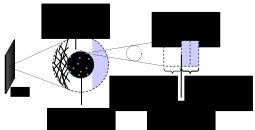
\includegraphics[width=0.65\linewidth]{3-PhaseChangeIonomer}%
    \label{fig:PhaseChangeIonomer}
  }\quad
  \subfloat[Gas to liquid]{
    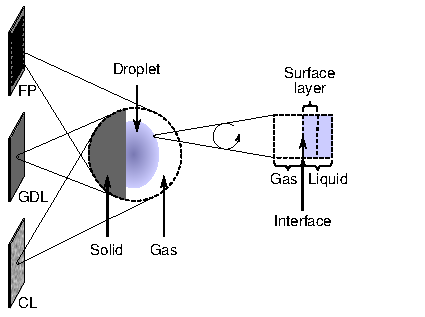
\includegraphics[width=0.65\linewidth]{3-PhaseChangeLiquid}%
    \label{fig:PhaseChangeLiquid}
  }
  \caption[Locations of the phase change processes]{Phase change occurs between the gas and \subref{fig:PhaseChangeIonomer} the ionomer in the catalyst layers (CLs) and \subref{fig:PhaseChangeLiquid} the liquid in the flow plates (FPs), gas diffusion layers (GDLs), and CLs}
  \label{fig:PhaseChangeContext}
  \glsadd{_l}\glsadd{_ionomer}
\end{figure}


\subsubsection{Equations}

The rate of condensation or absorption is given by the diffusive exchange equation (\ref{eq:DiffusiveExchange2}) for material ($\s{X} = \s{N}$, $\s{gamma} = \s{rho}$, $\partial\s{X}/\partial\s{gamma} = \s{V}$).\footnote{Phase change is purely diffusive.  As mentioned in \autoref{fn:NoAdvectiveMaterialExchange}, the advective exchange equation (\ref{eq:AdvectiveExchange1}) is not applicable to material exchange.}
\begin{equation}
  \label{eq:PhaseChange1a}
  \frac{8}{3\pi}\s{tau}[_c]\timessep\dot{N}\sub{_D}[ ][_i][_c] = \s{k}\sub{_i}[_c]\s{V}[_c]\group{\s{rho}[_i] - \s{rho}[_c]}
\end{equation}
where the subscript~c denotes the condensed or absorbed phase.  Since $\s{rho} = \s{N}/\s{V}$,
\begin{equation}
  \label{eq:PhaseChange2a}
  \frac{8}{3\pi}\s{tau}[_c]\timessep\dot{N}\sub{_D}[ ][_i][_c] = \s{k}\sub{_i}[_c]\s{N}[_c]\group{\frac{\s{rho}[_i]}{\s{rho}[_c]} - 1}
\end{equation}
We will assume that the species behaves as an isothermal ideal gas over the transition region or surface layer.  Under these conditions, \autoref{eq:GibbsFunction} evaluates to
\begin{equation}
  \s{g}[_i] - \s{g}[_c] = \s{T}[_c]\ln\group{\frac{\s{rho}[_i]}{\s{rho}[_c]}}
\end{equation}
Therefore, the rate of condensation or absorption can be written as
\begin{equation}
  \label{eq:PhaseChange}
  \boxed{\s{tau}\sub{_i}[_c]\sup{^prime}\timessep\dot{N}\sub{_D}[ ][_i][_c] = \s{N}[_c]\Group{\exp\group{\frac{\s{g}[_i] - \s{g}[_c]}{\s{T}[_c]}} - 1}}
\end{equation}
where \s{tau}[^prime]~is the effective collision interval, or the mean time between collisions that yield phase change:
\begin{equation}
  \label{eq:EffectiveCollisionInterval}
  \boxed{\s{tau}\sub{_i}[_c]\sup{^prime} = \frac{8}{3\pi\s{k}\sub{_i}[_c]}\s{tau}[_c]}
\end{equation}
In practice, $\s{tau}\sub{_i}[_c]\sup{^prime}$~is an empirical, tunable parameter.  Since we have assumed that the entire transition region is within the condensed phase, the gas is in equilibrium with the condition at the interface.
\begin{equation}
  \label{eq:PhaseChange3b}
  \boxed{\s{g}[_i] = \s{g}[_g]}
\end{equation}
where the subscript~\s{g} denotes the gas phase.  Therefore,
\begin{equation}
  \label{eq:PhaseChange4}
  \s{tau}\sub{_i}[_c]\sup{^prime}\timessep\dot{N}\sub{_D}[ ][_i][_c] = \s{N}[_c]\Group{\exp\group{\frac{\s{g}[_g] - \s{g}[_c]}{\s{T}[_c]}} - 1}
\end{equation}
This can also be written in terms of activity referenced to the condensed phase.
\begin{equation}
  \s{tau}\sub{_i}[_c]\sup{^prime}\timessep\dot{N}\sub{_D}[ ][_i][_c] = \s{N}[_c]\group{\s{a}[_g] - \s{a}[_c]}
\end{equation}
which is consistent with the common interpretation of activity as an effective, dimensionless concentration.


This model is appropriate for condensation and evaporation or absorption and desorption.  It should be noted that if the condensed phase is entirely absent ($\s{N}[_c] = 0$), there can be no condensation.  If phase change is included, the conditions are set so that some amount of material (as slight as it may be) always exists in the condensed or absorbed phase.

If the effective collision interval is zero ($\s{tau}\sub{_i}[_c]\sup{^prime} = 0$), then the phases will be in perfect equilibrium.  Then, it is no longer a dynamic process, and in general, there will be nonlinear systems of equations.  Since phase change is a diffusive process, the equilibration is irreversible.  Heat is generated in phase~\s{j} at the rate of $\dot{N}\sub{_D}[ ][_i][_j]\group{\s{g}[_i] - \s{g}[_j]}$ (discussed further in \autoref{sec:EnergyBalance}).  However,  this is zero for the gas phase due to \autoref{eq:PhaseChange3b}.  This excludes the latent heat, which is transferred via thermal advective exchange (\autoref{sec:ThermalAdvectiveExchange}).


\subsection{Drag and Translational Advection}
\label{sec:TranslationalExchange}

The translational exchange equations follow from the generalized exchange equations (\ref{eq:AdvectiveExchange2} and \ref{eq:DiffusiveExchange2}).  The exchanged quantity~(\s{X}) is the product of the amount of material and velocity~(\s{Phi}).  Both the intensive property $\partial\s{X}/\partial\s{N}$ %(or $\partial\s{Phi}/\partial\s{N}$)
and the diffusion-driving property~(\s{gamma}) are velocity~(\s{phi}).  The extensive property $\partial\s{X}/\partial\s{gamma}$ %(or $\partial\s{Phi}/\partial\s{phi}$)
is the amount of material~(\s{N}).


\subsubsection{Advection}


Advective translational exchange occurs in a stream of fluid that is undergoing phase change or reaction.  It is not significant in the reactions of a \n{PEMFC} since they occur at the surface of stationary electrodes.  However, the model includes advective translational exchange for completeness; it may be important in other devices.


In terms of translational exchange, \autoref{eq:AdvectiveExchange2} is the following:
\begin{equation}
  \label{eq:TranslationalAdvectiveExchange1}
  \dot{Phi}\sub{_A}[ ][_i][_j] = \dot{N}\sub{_i}[_j]\cdot
  \begin{cases}%
    \s{phi}[_j] & \text{if $\dot{N}\sub{_i}[_j] < 0$ (source),} \\
    \s{phi}[_i] & \text{if $\dot{N}\sub{_i}[_j] > 0$ (sink)}
  \end{cases}
\end{equation}
However, the product of the amount of material and velocity~(\s{Phi}) is not generally conserved.  Momentum, \s{mPhi}, is.  Therefore, we will multiply the previous equation by specific mass so that it can be written in terms of forces or rates of momentum:
\begin{equation}
  \label{eq:TranslationalAdvectiveExchange}
  \boxed{\dot{mPhi}\sub{_A}[ ][_i][_j] = \s{m}[_j]\dot{N}\sub{_i}[_j]\cdot
  \begin{cases}%
    \s{phi}[_j] & \text{if $\dot{N}\sub{_i}[_j] < 0$ (source),} \\
    \s{phi}[_i] & \text{if $\dot{N}\sub{_i}[_j] > 0$ (sink)}
  \end{cases}}
\end{equation}

The variable~\s{phi}[_i]~is the \emph{\n{conversion velocity}}, or the velocity at which the products are generated from the reactants during advective exchange.  Its value is a consequence of conservation at the interface (\autoref{eq:TranslationalBalanceInterface}).  Since advection and diffusion are independent, the sum of the advective forces ($\dot{mPhi}\sub{_A}[ ][_i][_j]$) over all of the interacting configurations is zero.  Using \autoref{eq:TranslationalAdvectiveExchange}, this is
\begin{equation}
  0 = \sum_{\s{j} \in \s{xi}[_i]}\s{m}[_j]\dot{N}\sub{_i}[_j]\cdot
  \begin{cases}%
    \s{phi}[_j] & \text{if $\dot{N}\sub{_i}[_j] < 0$ (source),} \\
    \s{phi}[_i] & \text{if $\dot{N}\sub{_i}[_j] > 0$ (sink)}
  \end{cases}
\end{equation}
where \s{xi}[_i]~is the set of the configurations that interact at transition~\s{i}.  The currents ($\dot{N}\sub{_i}[_j]$) are related by the stoichiometry of the phase change or reaction.
\begin{equation}
  \dot{N}\sub{_i}[_j] = \s{n}\sub{_i}[_j]\dot{N}[_i]
\end{equation}
where \dot{N}[_i]~is the rate of the transition~\s{i} and $\s{n}\sub{_i}[_j]$~is the stoichiometric coefficient of configuration~\s{j} with respect to transition~\s{i}.  Therefore,
\begin{equation}
  0 = \sum_{\s{j} \in \s{xi}[_i]}\s{m}\sub{_i}[_j]\s{n}\sub{_i}[_j]\cdot
  \begin{cases}%
    \s{phi}[_j] & \text{if $\s{n}\sub{_i}[_j]\dot{N}[_i] < 0$ (source),} \\
    \s{phi}[_i] & \text{if $\s{n}\sub{_i}[_j]\dot{N}[_i] > 0$ (sink)}
  \end{cases}
\end{equation}
Solving for the conversion velocity,
\begin{equation}
  \label{eq:ConversionVelocity1}
  \s{phi}[_i] = \frac{\sum_{\s{j}\in\text{source}}\left|\s{n}\sub{_i}[_j]\right|\s{m}[_j]\s{phi}[_j]}{\sum_{\s{j}\in\text{sink}}\left|\s{n}\sub{_i}[_j]\right|\s{m}[_j]}
\end{equation}
where the numerator is summed over the sourcing configurations (reactants) and the denominator is summed over the sinking configurations (products).  If the process is well-posed, it must conserve mass ($\sum_{\s{j}\in\text{source}}|\s{n}\sub{_i}[_j]|\s{m}[_j] = \sum_{\s{j}\in\text{sink}}|\s{n}\sub{_i}[_j]|\s{m}[_j]$), and
\begin{equation}
  \label{eq:ConversionVelocity2}
  \s{phi}[_i] = \frac{\sum_{\s{j}\in\text{source}}\left|\s{n}\sub{_i}[_j]\right|\s{m}[_j]\s{phi}[_j]}{\sum_{\s{j}\in\text{source}}\left|\s{n}\sub{_i}[_j]\right|\s{m}[_j]}
\end{equation}
Thus, the conversion velocity is the mass-weighted average of the velocities of the configurations consumed by the process.


\subsubsection{Diffusion}

For translational exchange, \autoref{eq:DiffusiveExchange2} is the following:
\begin{equation}
  \label{eq:TranslationalDiffusiveExchange1}
  \frac{8}{3\pi}\s{tau}[_j]\timessep\dot{Phi}\sub{_D}[ ][_i][_j] = \s{k}\sub{_i}[_j]\s{N}[_j]\group{\s{phi}[_i] - \s{phi}[_j]}
\end{equation}
This can be written as
\begin{equation}
  \label{eq:TranslationalDiffusiveExchange}
  \boxed{\s{mu}[_j]\timessep\dot{mPhi}\sub{_D}[ ][_i][_j] = \s{k}\sub{_i}[_j]\s{N}[_j]\group{\s{phi}[_i] - \s{phi}[_j]}}
\end{equation}
where \s{mu}[_j]~is the mobility:
\begin{equation}
  \label{eq:Mobility}
  \boxed{\s{mu} = \frac{8}{3\pi\s{m}}\s{tau}}
\end{equation}

The variable~\s{phi}[_i]~is the \emph{\n{mediation velocity}}.  Like the conversion velocity, it can be determined from conservation at the interface.  Since advection and diffusion are independent, the sum of the diffusion forces ($\dot{mPhi}\sub{_D}[ ][_i][_j]$) over all of the interacting configurations is zero.  Using \autoref{eq:TranslationalDiffusiveExchange}, this is
\begin{equation}
  0 = \sum_{\s{j} \in \s{xi}[_i]}\left.\group{\s{phi}[_i] - \s{phi}[_j]}\s{k}\sub{_i}[_j]\s{N}[_j]\middle/\s{mu}[_j]\right.
\end{equation}
where \s{xi}[_i]~is the set of all the interacting configurations at transition~\s{i}.  Solving for the mediation velocity,
\begin{equation}
  \label{eq:MediationVelocity}
  \s{phi}[_i] = \frac{\sum_{\s{j} \in \s{xi}[_i]}\left.\s{phi}[_j]\s{k}\sub{_i}[_j]\s{N}[_j]\middle/\s{mu}[_j]\right.}{\sum_{\s{j} \in \s{xi}[_i]}\left.\s{k}\sub{_i}[_j]\s{N}[_j]\middle/\s{mu}[_j]\right.}
\end{equation}
This indicates that the mediation velocity is a conductance-weighted average of the velocities of the interacting configurations.  The previous equation applies to each set~\s{xi} associated with each interaction~\s{i}.  Each set can have a different value of the mediation velocity.


\subsection{Thermal Conduction and Advection}
\label{sec:ThermalExchange}

The translational exchange equations follow from the generalized exchange equations (\ref{eq:AdvectiveExchange2} and \ref{eq:DiffusiveExchange2}).  The exchanged quantity~(\s{X}) is heat~(\s{Q}).  The intensive property $\partial\s{X}/\partial\s{N}$ is the product of specific entropy and temperature ($\partial\s{Q}/\partial\s{N} = \s{T}\partial\s{S}/\partial\s{N} = \s{T}\s{s}$).  The diffusion-driving property~(\s{gamma}) is temperature~(\s{T}).  The extensive property $\partial\s{X}/\partial{\s{gamma}}$ is heat capacity~(\s{C}).  The heat capacity is isobaric (\s{C}[_p]), since the pressures of the configurations are assumed to be at equilibrium (see \autoref{sec:AmagatsLaw}).


\subsubsection{Advection}
\label{sec:ThermalAdvectiveExchange}

In terms of thermal exchange, \autoref{eq:AdvectiveExchange2} is
\begin{equation}
  \label{eq:ThermalAdvectiveExchange}
  \boxed{\dot{Q}\sub{_A}[ ][_i][_j] = \dot{N}\sub{_i}[_j]\cdot
  \begin{cases}%
    \group{\s{s}\s{T}}\sub{_j} & \text{if $\dot{N}\sub{_i}[_j] < 0$ (source),} \\
    \group{\s{s}\s{T}}\sub{_i} & \text{if $\dot{N}\sub{_i}[_j] > 0$ (sink)}
  \end{cases}}
\end{equation}

where \s{j}~is a configuration that participates in reaction or phase change~\s{i}.  It is important to note that \dot{Q}[_A] is advective.  It is different from \dot{Q}[_D], which is the rate of thermal diffusion or conduction.  In the energy balance (\autoref{eq:EnergyBalance}), the $\s{s}\s{T}$ factor combines with the specific Gibbs energy~(\s{g}) to give the specific enthalpy~(\s{h}) that is transferred with the process (reaction or phase change).  The rate of thermal energy due to $\sum\dot{N}[_j]\group{\s{s}\s{T}}[_j]$ or $\dot{N}\sum\s{n}[_j]\group{\s{s}\s{T}}[_j]$ over a process (where the subscript~\s{i} has been dropped) is split stoichiometrically (not by mass) among the products (sinks).  The intensive properties of the reactants (sources) are not directly affected due to the conditional factor in \autoref{eq:ThermalAdvectiveExchange}.  If the process occurs near equilibrium, then $\sum\s{n}[_j]\s{g}[_j]$ is nearly zero and $\sum\s{n}[_j]\group{\s{s}\s{T}}[_j]$ is nearly $\sum\s{n}[_j]\s{h}[_j]$, the enthalpy of the reaction or phase change.  If the process is not at equilibrium, heat is produced at the rate of $\dot{N}\sum\s{n}[_j]\s{g}[_j]$.  This is irreversible because the process always occurs towards lower specific Gibbs energy.\footnote{This was evident from the equation for the rate of phase change (\ref{eq:PhaseChange}) and is also the case in electrochemical reactions, inclusive of the electrical work potential (\autoref{sec:Reaction}).}

The property $\group{\s{s}\s{T}}[_i]$~is the thermal conversion property---the product of specific entropy and temperature at which the products are generated from the reactants during advective exchange.  Its value is a consequence of conservation at the interface (\autoref{eq:ThermalBalanceInterface}).  Since advection and diffusion are independent, the sum of the advective rates ($\dot{Q}\sub{_A}[ ][_i][_j]$) over all of the interacting configurations is zero.  Using \autoref{eq:ThermalAdvectiveExchange}, this is
\begin{equation}
  0 = \sum_{\s{j} \in \s{xi}[_i]}\dot{N}\sub{_i}[_j]\cdot
  \begin{cases}%
    \group{\s{s}\s{T}}[_j] & \text{if $\dot{N}\sub{_i}[_j] < 0$ (source),} \\
    \group{\s{s}\s{T}}[_i] & \text{if $\dot{N}\sub{_i}[_j] > 0$ (sink)}
  \end{cases}
\end{equation}
where \s{xi}[_i]~is the set of the configurations that interact at transition~\s{i}.  The currents ($\dot{N}\sub{_i}[_j]$) are related by the stoichiometry of the phase change or reaction.
\begin{equation}
  \dot{N}\sub{_i}[_j] = \s{n}\sub{_i}[_j]\dot{N}[_i]
\end{equation}
where $\dot{N}[_i]$ is the rate of the transition~\s{i} and $\s{n}\sub{_i}[_j]$~is the stoichiometric coefficient of configuration~\s{j} with respect to transition~\s{i}.  Therefore,
\begin{equation}
  0 = \sum_{\s{j} \in \s{xi}[_i]}\s{n}\sub{_i}[_j]\cdot
  \begin{cases}%
    \group{\s{s}\s{T}}[_j] & \text{if $\s{n}\sub{_i}[_j]\dot{N}[_i] < 0$ (source),} \\
    \group{\s{s}\s{T}}[_i] & \text{if $\s{n}\sub{_i}[_j]\dot{N}[_i] > 0$ (sink)}
  \end{cases}
\end{equation}
Solving for the thermal conversion property,
\begin{equation}
  \label{eq:ThermalConversionProperty}
  \group{\s{s}\s{T}}[_i] = \frac{\sum_{\s{j}\in\text{source}}\left|\s{n}\sub{_i}[_j]\right|\group{\s{s}\s{T}}[_j]}{\sum_{\s{j}\in\text{sink}}\left|\s{n}\sub{_i}[_j]\right|}
\end{equation}
where the numerator is summed over the sourcing configurations (reactants) and the denominator is summed over the sinking configurations (products).  Thus, the thermal conversion property is the stoichiometrically-weighted average of the specific entropy-temperature products (or specific enthalpy-specific Gibbs energy differences) of the configurations consumed by the process.



\subsubsection{Diffusion}

For thermal diffusion (i.e., thermal conduction), \autoref{eq:DiffusiveExchange2} is
\begin{equation}
  \label{eq:ThermalDiffusiveExchange1}
  \frac{8}{3\pi}\s{tau}[_j]\timessep\dot{Q}\sub{_D}[ ][_i][_j] = \s{k}\sub{_i}[_j]\s{C}\sub{_p}[_j]\group{\s{T}[_i] - \s{T}[_j]}
\end{equation}
This can be written as
\begin{equation}
  \label{eq:ThermalDiffusiveExchange}
  \boxed{\s{nu}[_j]\timessep\dot{Q}\sub{_D}[ ][_i][_j] = \s{k}\sub{_i}[_j]\s{N}[_j]\group{\s{T}[_i] - \s{T}[_j]}}
\end{equation}
where \s{nu}[_j]~is called thermal \emph{\n{independity}} here.\footnote{This is the thermal analog of mobility, but there is no established name.  It is not called resistivity.  Resistivity is resistance times the quotient of area and length, whereas independity is resistance (or \emph{\n{independence}}) times the amount of material.}  It is defined by
\begin{equation}
  \label{eq:ThermalIndependity}
  \boxed{\s{nu} = \frac{8}{3\pi\s{c}[_p]}\s{tau}}
\end{equation}

The variable~\s{T}[_i]~is the \emph{\n{mediation temperature}}.  Like the thermal conversion property, it can be determined from conservation at the interface.  Since advection and diffusion are independent, the sum of the heat flow rates ($\dot{Q}\sub{_D}[ ][_i][_j]$) over all of the interacting configurations is zero.  Therefore, the sum of \autoref{eq:ThermalDiffusiveExchange} is
\begin{equation}
  0 = \sum_{\s{j} \in \s{xi}[_i]}\left.\group{\s{T}[_i] - \s{T}[_j]}\s{k}\sub{_i}[_j]\s{N}[_j]\middle/\s{nu}[_j]\right.
\end{equation}
where \s{xi}[_i]~is the set of all the interacting configurations at transition~\s{i}.  Solving for the mediation temperature,
\begin{equation}
  \label{eq:MediationProperty}
  \s{T}[_i] = \frac{\sum_{\s{j} \in \s{xi}[_i]}\left.\s{T}[_j]\s{k}\sub{_i}[_j]\s{N}[_j]\middle/\s{nu}[_j]\right.}{\sum_{\s{j} \in \s{xi}[_i]}\left.\s{k}\sub{_i}[_j]\s{N}[_j]\middle/\s{nu}[_j]\right.}
\end{equation}
This indicates that the mediation temperature is a conductance-weighted average of the temperatures of the configurations interacting by diffusion.  The previous equation applies to each set~\s{xi} associated with each interaction~\s{i}.  Each set can have a different value of the mediation temperature.


\section{Exchange Properties}
\label{sec:ExchangeProperties}

The base factor in the diffusive exchange properties is the collision interval or the mean time between collisions.  It depends on the thermodynamic state and possibly other properties, but it can be estimated from kinetic theory under the following assumptions~\cite{Present1958}:
\begin{enumerate*}
  \item The particles are smooth and rigid but elastic spheres with identical radii.  This is the ``billiard-ball'' assumption.  It implies that the collisions are instantaneous and conserve kinetic energy.
  \item The mean free path, or the average distance a particle travels between collisions, is much larger than the diameter of a particle.
  \item The speeds of the particles follow the Maxwell-Boltzmann distribution.
\end{enumerate*}

With these assumptions, the mean free path is
\begin{equation}
  \label{eq:MeanFreePath}
  \boxed{\s{lambda} = \frac{\s{v}}{\sqrt{2}\pi\s{d}^2\s{q}}}
\end{equation}
where \s{v}~is the specific volume of the particles (reciprocal of concentration), \s{d}~is the specific rigid-sphere or Van der Waals diameter, and \s{q}~is the particle number representing a single particle~\cite{Present1958, Cercignani1962}. %\cite[pp.~31--32]{Present1958}, \cite[p.~229]{Cercignani1962}
The denominator is the product of the intercept area per particle with particles of the same type ($\pi\s{d}^2\s{q}$) and a correction due to the Maxwell-Boltzmann distribution ($\sqrt{2}$).\footnote{It is counterintuitive that the distribution of molecular speeds has an effect on the mean free path, but this has been established in the literature \cite[p.~32]{Present1958}.}  The derivation is beyond the present scope (see \cite[pp.~31--32]{Present1958} and \cite[p.~229]{Cercignani1962}).  The collision interval is the mean free path divided by the mean thermal speed ($\sqrt{8\s{T}/\pi\s{m}}$):
\begin{equation}
  \label{eq:CollisionInterval}
  \boxed{\s{tau} = \s{lambda}\sqrt{\frac{\pi\s{m}}{8\s{T}}}}
\end{equation}
The collision interval is called the relaxation time in solid state physics~\cite{Ashcroft1976}.  For a typical species, the collision interval is small.  For oxygen as an ideal gas at \SI{25}{\celsius} and 21\% of atmospheric pressure, the specific volume~(\s{v}) is \SI{0.12}{m^3/mol}.  The diameter of a particle is approximately \SI{220}{pm}; therefore the mean free path is approximately \SI{0.9}{\micro\metre} and the collision interval is approximately \SI{2}{ns}.

The effective collision interval, which is used for phase change, can be determined from the collision interval using \autoref{eq:EffectiveCollisionInterval}.  Mobility and thermal independity can be determined from the collision interval using Equations \ref{eq:Mobility} and \ref{eq:ThermalIndependity}.  Due to the assumptions implicit in the diffusive exchange equation (\ref{eq:DiffusiveExchange2}), the equations for the effective collision interval, mobility, and thermal independity are only taken to be estimates.  However, they are useful if more precise data is not available.


\section{Transport Equations}
\label{sec:Transport}

% **current is linear, not velocity.

\begin{contextbox}
  Highlights:
  \begin{itemize*}
    \item The model describes the transport of every species individually, even in purely advective flow.  However, the diffusive exchange of translational momentum (\autoref{sec:Reaction}) tends to couple the velocities of the species and thus the rates of advective transport.
    \item A general transport equation is proposed to handle upstream discretization.  It meets the exact solution to a mixed advection\slash{}diffusion problem~\cite{Patankar1980}.
    \item The transport equation changes continuously from neutral discretization under pure diffusion to complete upstream discretization in the limiting case of pure advection.  This avoids switching events that could slow the simulation if diffusion were not included.
    \item The model is expressed in resistivity instead of conductivity so that it is well-posed under all representable values.
    \item The model allows zero or finite dynamic compressibility.  The reciprocal, bulk viscosity, is rarely studied~\cite{Rah1999} and seldom included in fluid simulations~\cite{Meier2005}, let alone fuel cell simulations.  The associated effect may be neglected for monoatomic ideal gases and incompressible fluids~\cite{Kerkhof2005ChemEngSci, Meier2005}, but following a plausible formation (see \autoref{sec:MaterialTransport}) the effect is dominant for lightweight particles such as electrons.
    \item The material transport equation combines the effects of self diffusivity and bulk viscosity to describe material advection and diffusion.  That way, the same equations can describe the primarily advective flow down the channels of a \n{PEMFC} and the primarily diffusive flow through the layers.
  \end{itemize*}
\end{contextbox}

% \begin{figure}[!htb]
%   \newcommand{\vgap}{\vphantom{Transport}}
%   \centering
%   \begin{tikzpicture}
%     [level distance=1.5cm,
%      level 2/.style={level distance=1.1cm}]
%     \Tree[.FC\\Model
%            [.{Processes\vgap}
%               [.{Transport\vgap}
%                 [.{Advection\vgap} ]
%                 [.{Diffusion\vgap} ] ] ] ]
%   \end{tikzpicture}
%   \caption{Types of transport processes in the fuel cell model}
% \end{figure}

\emph{\N{transport}} is the transfer of a conserved quantity between adjacent regions.  Like exchange (\autoref{sec:Exchange}), it is due to advection and diffusion.  Advective transport is the transfer of the quantity along with a sustained transfer of material between regions.  Diffusive transport is the transfer of the quantity due only to collisions or thermal agitation of the particles, without a sustained material transfer.  In diffusion, a particle leaves one region with the specific quantity (or particle-average amount of the quantity) within the configuration and returns with the specific quantity of the other configuration.  This brings certain intensive properties---concentration, velocity, and temperature---into equilibrium among the configurations.  Since these properties are sufficient to set the thermodynamic state, other properties (e.g., pressure) equilibrate as well.

In transport, unlike exchange, advection and diffusion are not independent.  The transport equations are based on the following assumptions:
\begin{enumerate*}

  \item Transport of material, momentum, and energy only occurs between like configurations (e.g., liquid water).  Bulk transport is only the net, macroscopic effect of individual species flows.  The inter-configurational effects (e.g., between liquid water and water vapor) are described within a region via exchange (\autoref{sec:Exchange}).

  \item \label{itm:AssumeAligned} The coordinate system is aligned with the principle axes of transport.  For example, if a phase is stratified within a region, the layers must be parallel to one of the planes in the rectilinear grid.  This implies that a gradient which induces diffusion along an axis does not induce diffusion along axes orthogonal to it~\cite{Bejan2006}.%[pp.~691--692].
  \item There is no radiative heat transfer.
\end{enumerate*}

The total rate of transport of a quantity~\s{X} into configuration~\s{j} from boundary~\s{i} is the sum of the advective and diffusive rates:
\begin{equation}
  \label{eq:Transport}
  \dot{X}[_i] = \dot{X}\sub{_A}[ ][_i] + \dot{X}\sub{_D}[ ][_i]
\end{equation}
This is the same as for exchange (\autoref{eq:Exchange}) except \s{i}~stands for a boundary rather than a transition.  The subscript~\s{j} has been removed because the equations of this section all pertain to a single configuration.  The advective and diffusive terms will be evaluated separately.


\noindent\underline{\textbf{Advection}}

The rate of advective transport is the product of the current and the change in the transported quantity with respect to the material.
\begin{equation}
  \label{eq:AdvectiveTransport}
  \dot{X}\sub{_A}[ ][_i] = \dot{N}[_i]\diffp{\s{X}}{\s{N}}[_i]
\end{equation}
where $\dot{N}[_i]$ is the total (advective plus diffusive) rate of material transport of a configuration through boundary~\s{i} into a region.  The partial derivative $(\partial\s{X}/\partial\s{N})\sub{_i}$ is an intensive property at the boundary.  This equation is general; in fact, it is the same as for advective exchange (\autoref{eq:AdvectiveExchange1}, without subscript \s{j}).


\noindent\underline{\textbf{Diffusion}}

Like for exchange (\autoref{sec:Exchange}), we can consider the diffusive transport rate to be the material derivative or the transport rate experienced by the particles themselves.\footnote{See the discussion at the end of this section.}
\begin{equation}
  \label{eq:DiffusiveTransport1}
  \dot{X}\sub{_D}[ ][_i] = \Diff{\s{X}[^prime]}{\s{t}}[_i]
\end{equation}
where $(\mathrm{D}\s{t})\sub{_i}$ is the time for a particle to pass from the boundary to the center of the region.  It is the product of \begin{inparaenum}[(1)]\item the mean collision interval~(\s{tau}), \item a logistic function for upstream discretization ($1/(1 + \exp(\mp\s{Pe}/2))$, described below), \item a factor of three due to the geometry of randomly-moving particles striking a boundary \cite[p.~33--35]{Present1958}, \item a factor to account for the effect of other phases on transport length and available cross-section area~(\s{k}), and \item the number of collisions required to span the distance from the boundary to the center of the region\end{inparaenum}.  That number is the reciprocal of the Knudsen number~(\s{Kn}) or the length across the region divided the mean free path ($1/\s{Kn} = \s{L}/\s{lambda}$).  The effective difference in the transported quantity $(\mathrm{D}\s{X}[^prime])\sub{_i}$ is the actual difference $(\mathrm{D}\s{X})\sub{_i}$ divided by the number of collisions required to span the distance between the boundary and the center (again, the reciprocal of the Knudsen number).  We will assume that the transported quantity is linear with respect to the driving property~(\s{gamma}); therefore, $(\mathrm{D}\timessep\s{X})\sub{_i} = (\s{gamma}[_i] - \s{gamma})(\partial\s{X}/\partial\s{gamma})$.  The following assumptions have also been implied:
\begin{enumerate*}
  \item The collision events are frequent enough for the average collision interval to be meaningful.  This implies that the mean free path, or the average distance traveled between collisions, is much smaller than the length scale of the problem.  It is not the case for example in effusion.
  \item Between collisions the particles have no influence on one another.
  \item The properties carried by a particle depend only on those of the last particle with which it collided.
\end{enumerate*}
It follows that
\begin{equation}
  \label{eq:DiffusiveTransport2}
  3\s{tau}\timessep\dot{X}\sub{_D}[ ][_i] = \s{k}[_i]\s{Kn}\sub{_i}^2\timessep\diffp{\s{X}}{\s{gamma}}\group{\s{gamma}[_i] - \s{gamma}}\group{1 + e^{\mp\s{Pe}[_i]/2}}
\end{equation}
where the negative of $\mp$ is for the negative side of the region along an axis and the positive is for the positive side.\footnote{This convention is used throughout the chapter.  Likewise, the $\pm$ operator indicates that the positive is for the negative side of the region and the negative is for the positive side.}  This can be written as
\begin{equation}
  \label{eq:DiffusiveTransport3}
  \s{R}[_i]\timessep\dot{X}\sub{_D}[ ][_i] = \group{\s{gamma}[_i] - \s{gamma}}\group{1 + e^{\mp\s{Pe}[_i]/2}}
\end{equation}
where the generalized resistance is
\begin{equation}
  \label{eq:Resistance1}
  \s{R}[_i]= \left.\frac{3\s{tau}}{\s{k}[_i]\s{Kn}\sub{_i}^2}\middle/\diffp{\s{X}}{\s{gamma}}\right.
\end{equation}
The resistance can be written as
\begin{equation}
  \label{eq:Resistance2}
  \s{R}[_i]= \frac{\s{r}\s{L}[_i]}{\s{k}[_i]\s{A}[_i]}
\end{equation}
where the resistivity is
\begin{equation}
  \label{eq:Resistivity}
  \s{r} = \left.\frac{3\s{tau}[_i]\s{V}}{\s{lambda}[_i]^2}\middle/\diffp{\s{X}}{\s{gamma}}\right.
\end{equation}
using the definition of the Knudsen number ($\s{Kn} \equiv \s{lambda}/\s{L}$).
In terms of resistivity, the diffusive transport equation is:
\begin{equation}
  \label{eq:DiffusiveTransport4}
  \s{r}\timessep\dot{X}\sub{_D}[ ][_i] = \frac{\s{k}[_i]\s{A}[_i]}{\s{L}[_i]}\group{\s{gamma}[_i] - \s{gamma}}\group{1 + e^{\mp\s{Pe}[_i]/2}}
\end{equation}
If two adjacent regions have zero resistivity, their intensive driving properties~(\s{gamma}) will be equal.  The transported quantity will flow between the regions without loss in order to meet that requirement and the number of dynamic states will be reduced by one.

The model uses resistance and resistivity instead of conductance and conductivity (the reciprocals) because the equations are numerically well-posed for zero resistivity and resistance but not for zero conductance and conductivity.  Values of zero can be directly represented in the modeling language but infinite values cannot (see \autoref{chap:Implementation}).  Infinite values of resistivity (zero conductivity) can be represented by directly imposing zero flow rate (by a disconnected interface; see \autoref{chap:Implementation}).

The logistic factor $1/(1 + \exp(-\s{Pe}/2))$ introduces upstream discretization.  It changes the effective transport length depending on the direction and the magnitude of advection.  The P\'eclet number, \s{Pe}, is the dimensionless rate of advection from the interaction into the configuration.  The factor of one half appears in the exponential because, by default, half of the resistance is to either side of the region along the axis of transport.  In the P\'eclet number, the rate of advection is normalized by the rate of diffusion:
\begin{equation}
  \label{eq:Peclet1}
  \s{Pe} \equiv \left.\dot{X}[_A]\middle/\dot{X}[_D]\right.
\end{equation}
Using the rate of advection from \autoref{eq:AdvectiveTransport} and the rate of diffusion across a region (\autoref{eq:DiffusiveTransport3} as in \autoref{eq:DiffusiveTransportRegion}) at a differential level along with the definition of resistance (\autoref{eq:Resistance2}),
\begin{equation}
  \label{eq:Peclet2}
  \s{Pe} = \frac{\s{R}\dot{N}}{\mathrm{d}\s{gamma}}\diffp{\s{X}}{\s{N}}
\end{equation}
where the subscripts have been dropped.  Taking the current to be advective ($\dot{N} = \s{phi}\partial\s{N}/\partial\s{x} = \s{phi}\partial\s{N}/\s{L}$),
\begin{equation}
  \label{eq:Peclet3}
  \s{Pe} = \frac{\s{R}\s{phi}}{\s{L}}\diffp{\s{X}}{\s{gamma}}
\end{equation}
In terms of resistivity,
\begin{equation}
  \label{eq:Peclet4}
  \s{Pe} = \frac{\s{r}\s{phi}}{\s{k}\s{A}}\diffp{\s{X}}{\s{gamma}}
\end{equation}
where $\partial\s{X}/\partial\s{gamma}$ is an extensive material property.   This implies that the P\'eclet number is extensive as well.  Its magnitude increases as the length of the region along the transport axis increases.\footnote{Although length appears in the denominator of \autoref{eq:Peclet3}, it is canceled by the length factor of the resistance which is in the numerator.  This leaves $\partial\s{X}/\partial\s{gamma}$, which is extensive.}

The P\'eclet number tends to zero at the differential level of discretization or as the velocity becomes zero.  Then, the transport equation (\ref{eq:DiffusiveTransport3}) reduces to a typical diffusion relationship.
\begin{equation}
  \s{R}[_i]\dot{X}[_i] = 2\group{\s{gamma}[_i] - \s{gamma}}
\end{equation}
where the flow rate is evaluated at one side rather than between the locations of the properties.  The factor of two appears because the property difference ($\s{gamma}[_i] - \s{gamma}$) spans only half the length of the region.  We can consider the factor of $1/(1 + e^{\mp\s{Pe}/2})$ in the general transport equation (\ref{eq:DiffusiveTransport3}) to be a length scaling factor which is one half in this case.  With a length factor of one half, the transport equation (e.g., \ref{eq:DiffusiveTransport4}) implements the central difference scheme~\cite{Majumdar2005}. %[p\. 310--311] 

As the P\'eclet number becomes large, the length factor becomes one for the upstream side and zero for the downstream side.  The property in the region is weakly coupled to the upstream boundary and strongly coupled to the downstream boundary.  Equivalently, from the perspective of a boundary, the value of the property at the interface between regions is nearly the value in the upstream region.  The downstream region determines the diffusion rate.  The limiting cases are listed in \autoref{tab:TransportLimits}, where the subscript n indicates the negative side of a region along an axis and p indicates the positive side.  As stated by Patankar~\cite{Patankar1980},%[p.~20]
\begin{longquote}
    ``It is true that the one-way nature of a space coordinate is a one-way process, but diffusion (which is always present) has two-way influences.  However, when the flow rate is large, convection overpowers diffusion and thus makes the space coordinate nearly one-way.''
\end{longquote}
Here, the term ``advection'' is used instead of ``convection'' because convection is the serial combination of diffusion and advection, at least in the thermal context.

\begin{table}[hbt]
  \caption{Limiting cases of the transport equation}%
  \label{tab:TransportLimits}
  \begin{tabular}{ccc}
    \toprule
    \textbf{P\'eclet Number} & \textbf{Negative-side} & \textbf{Positive-side} \\
    ($\s{Pe}[_neg] = \s{Pe}[_pos]$) & \textbf{equation} & \textbf{equation} \\
    \midrule
    $\begin{aligned}%
       -&\infty \\
       &0 \\
       &\infty
     \end{aligned}$ &
    $\begin{aligned}%
       \s{gamma}[_neg] &= \s{gamma} \\
       \s{R}\dot{X}[_neg] &= 2\group{\s{gamma}[_neg] - \s{gamma}} \\
       \s{R}\dot{X}[_neg] &= \s{gamma}[_neg] - \s{gamma}[_pos]
     \end{aligned}$ &
    $\begin{aligned}%
       \s{R}\dot{X}[_pos] &= \s{gamma}[_pos] - \s{gamma}[_neg] \\
       \s{R}\dot{X}[_pos] &= 2\group{\s{gamma}[_pos] - \s{gamma}} \\
       \s{gamma}[_pos] &= \s{gamma}
     \end{aligned}$ \\
    \bottomrule
  \end{tabular}
\end{table}

If the resistivity is infinite, the transport equation reduces to the upwind scheme (also known as the upwind-difference scheme, upstream-difference scheme, and donor-cell method)~\cite{Patankar1980}. % See also \cite[p.~312]{Majumdar2005}.
The exponential switches immediately upon flow reversal.  The property at the interface is exactly the property of the upstream region.  The downstream region imposes the diffusion rate, which is zero.

As long as the resistivity is finite, the property changes continuously between the limiting cases of purely advective flow in each direction.  If we implement the transport equation (\ref{eq:DiffusiveTransport3}) twice---once for each boundary of a region along an axis---and place the restriction that the quantity is not stored in the region ($0 = \dot{X}[_neg] + \dot{X}[_pos]$), then
\begin{equation}
  \s{gamma}  = \frac{\s{gamma}[_pos]\group{1 + e^{\s{Pe}[_pos]/2}} + \s{gamma}[_neg]\group{1 + e^{-\s{Pe}[_neg]/2}}}{2 + e^{\s{Pe}[_pos]/2} + e^{-\s{Pe}[_neg]/2}}
\end{equation}
If the P\'eclet numbers of the two boundaries are equal ($\s{Pe} = \s{Pe}[_neg] = \s{Pe}[_pos]$), then
\begin{equation}
  \label{eq:MixingRegion}
  \frac{\s{gamma} - \s{gamma}[_neg]}{\s{gamma}[_pos] - \s{gamma}[_neg]} = \frac{1}{1 + e^{-\s{Pe}/2}}%
\end{equation}
where the right side is the logistic function of $\s{Pe}/2$.  \autoref{fig:AdvDiffRegion} shows the sigmoid curve which it represents.  In a similar manner, since there is no storage at an interface (as required by Equations \ref{eq:MaterialBalanceInterface}, \ref{eq:TranslationalBalanceInterface}, and \ref{eq:ThermalBalanceInterface}), the property at the interface between two regions is given by
\begin{equation}
  \label{eq:Mixing}
  \frac{\s{gamma} - \s{gamma}_1}{\s{gamma}_2 - \s{gamma}_1} = \frac{\s{R}_1\group{1 + e^{-\s{Pe}/2}}}{\s{R}_1\group{1 + e^{-\s{Pe}/2}} + \s{R}_2\group{1 + e^{\s{Pe}/2}}}%
  \glsadd{_123}
\end{equation}
where \s{gamma} (without a subscript) now represents the value of the property at the interface rather than the value in a region.  The subscript 1 indicates the first region and 2 indicates the second region.  Positive P\'eclet numbers are directed from the first to the second region.  If the regions have identical resistances ($\s{R}_1 = \s{R}_2$), this reduces to the same logistic function as for a single region except reflected over the $\s{Pe} = 0$ axis:
\begin{equation}
  \label{eq:MixingMidplane}
  \frac{\s{gamma} - \s{gamma}_1}{\s{gamma}_2 - \s{gamma}_1} = \frac{1}{1 + e^{\s{Pe}/2}}%
  \glsadd{_123}
\end{equation}
This means that an interface's property is biased towards the source whereas a region's property is biased towards the exit.  \autoref{fig:AdvDiffInterface} shows the relation in contrast to \autoref{fig:AdvDiffRegion}.

\begin{figure}[htbp]
  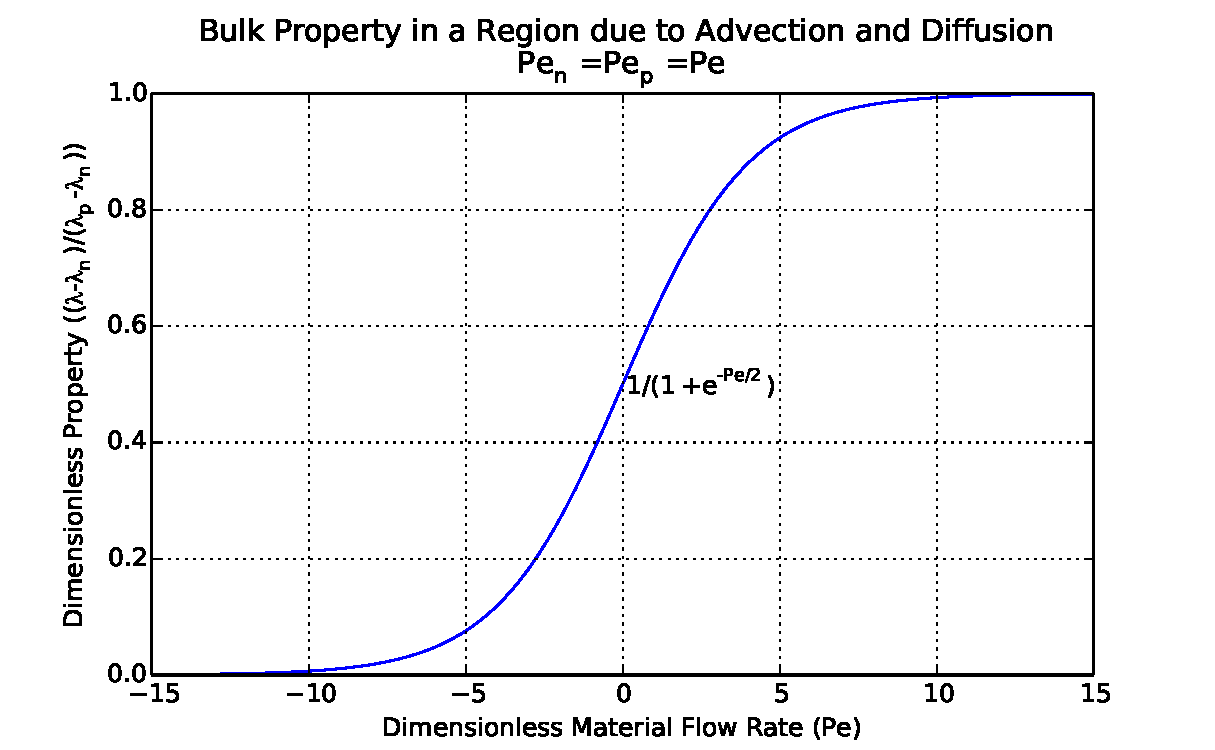
\includegraphics[width=0.9\linewidth]{3-AdvDiffRegion}%
  \caption{Property in the bulk of a region due to advection and diffusion}%
  \label{fig:AdvDiffRegion}
\end{figure}

\begin{figure}[htbp]
  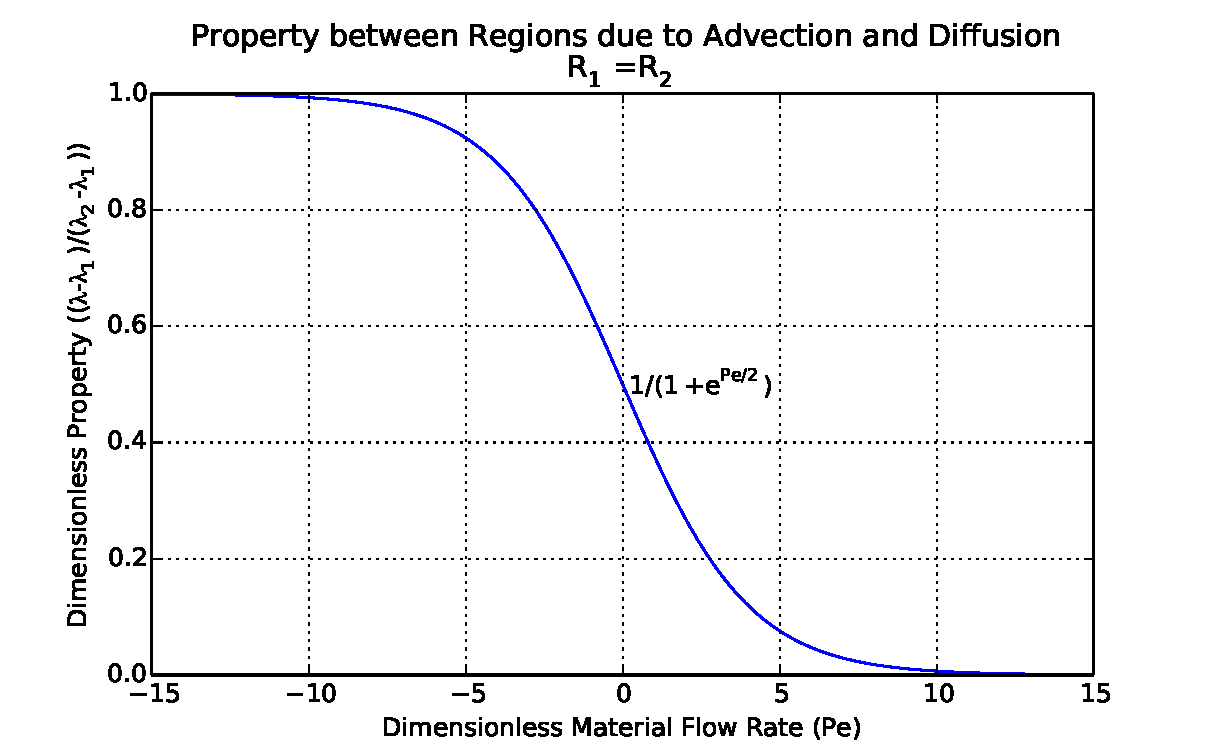
\includegraphics[width=0.9\linewidth]{3-AdvDiffInterface}%
  \caption{Property at the interface between regions due to advection and diffusion}%
  \label{fig:AdvDiffInterface}
\end{figure}

\autoref{eq:Mixing} can be used to provide the profile of the property between the centers of adjacent regions.  If we assume that the resistivity and cross-sectional area are uniform, \autoref{eq:Resistance1} implies that
\begin{equation}
  \frac{\s{gamma} - \s{gamma}_1}{\s{gamma}_2 - \s{gamma}_1} = \frac{\s{L}_1\group{1 + e^{-\s{Pe}/2}}}{\s{L}_1\group{1 + e^{-\s{Pe}/2}} + \s{L}_2\group{1 + e^{\s{Pe}/2}}}%
  \glsadd{_123}
\end{equation}
where $\s{L}_1$ is the length across region 1 and $\s{L}_2$ is the length across region 2.  If we vary the position of the interface while keeping the center-to-center distance the same (constant $\s{L} = (\s{L}_1 + \s{L}_2)/2$), we can express the value of the property as a function of position.
\begin{equation}
  \frac{\s{gamma} - \s{gamma}_1}{\s{gamma}_2 - \s{gamma}_1} = \frac{\s{x}[^star]\group{1 + e^{-\s{Pe}/2}}}{\s{x}[^star]\group{1 + e^{-\s{Pe}/2}} + \group{1 - \s{x}[^star]}\group{1 + e^{\s{Pe}/2}}}%
  \glsadd{_123}
\end{equation}
where $\s{x}[^star] = (\s{x} - \s{x}_1)/\s{L}$ is the dimensionless position between the first and second region as a function of~\s{x}, the absolute position of the interface.  This can be simplified to
\begin{equation}
  \label{eq:MixingProfile}
  \frac{\s{gamma} - \s{gamma}_1}{\s{gamma}_2 - \s{gamma}_1} = \frac{1}{1 + \group{\frac{1}{\s{x}[^star]} - 1}e^{\s{Pe}/2}}%
  \glsadd{_123}
\end{equation}
\autoref{fig:AdvDiffProfile} shows the resulting profile for various P\'eclet numbers (solid lines).  The profile is linear under pure diffusion ($\s{Pe} = 0$).  Otherwise, the profile is biased towards the property of the source.  The profile increases or decreases monotonically.  \autoref{eq:MixingProfile} reduces to \autoref{eq:MixingMidplane} when $\s{x}[^star] = 1/2$, as shown in the figure.

For comparison, Patankar~\cite{Patankar1980} provides the solution to the following general advection\slash{}diffusion equation under the condition of no material storage due to advection ($\mathrm{d}\s{I}/\mathrm{d}\s{x} = 0$) and no storage of the transported quantity due to combined advection and diffusion ($\mathrm{d}\dot{X}/\mathrm{d}\s{x} = 0$).  
\begin{equation}
  \dot{X} = \s{gamma}\s{I} - \frac{\s{A}}{\s{r}}\nabla\s{gamma}
\end{equation}
The equation has been refactored here under the assumption of uniform cross-sectional area.  The solution is
\begin{equation}
  \label{eq:PropertyProfile}
  \frac{\s{gamma} - \s{gamma}_1}{\s{gamma}_2 - \s{gamma}_1} = \frac{1 - e^{\s{Pe}\s{x}/\s{L}}}{1 - e^{\s{Pe}}}
  \glsadd{_123}
\end{equation}
where \s{L}~is the center-to-center distance between regions and \s{x}~is the position.  Note that this equation contains a numerical singularity in the case of pure diffusion ($\s{Pe} = 0$).  It matches \autoref{eq:MixingProfile} when $\s{x}[^star] = 1/2$, as shown by \autoref{fig:AdvDiffProfile}.  However, the model and the Patankar's solution are different at other positions.  This may be due to one of the following reasons: \begin{inparaenum}[(1)] \item the model is based on the requirement that the flow rate of the quantity out of one region is the flow rate into the other ($\dot{X}_{1\text{p}} + \dot{X}_{2\text{n}} = 0\glsadd{_pos}\glsadd{_neg}$ at the interface plane) whereas Patankar's solution is based on the requirement that there is no storage in a differential space around the interface ($\mathrm{d}\dot{X}/\mathrm{d}\s{x} = 0$) or \item the assumption of equal P\'eclet numbers (used in the derivation of \autoref{eq:MixingProfile} from \autoref{eq:Mixing}) is unreasonable\end{inparaenum}.  The P\'eclet number is extensive in nature (as mentioned previously), so it may not be appropriate to assume that it remains equal as the adjacent regions are resized.

\begin{figure}[htb]
  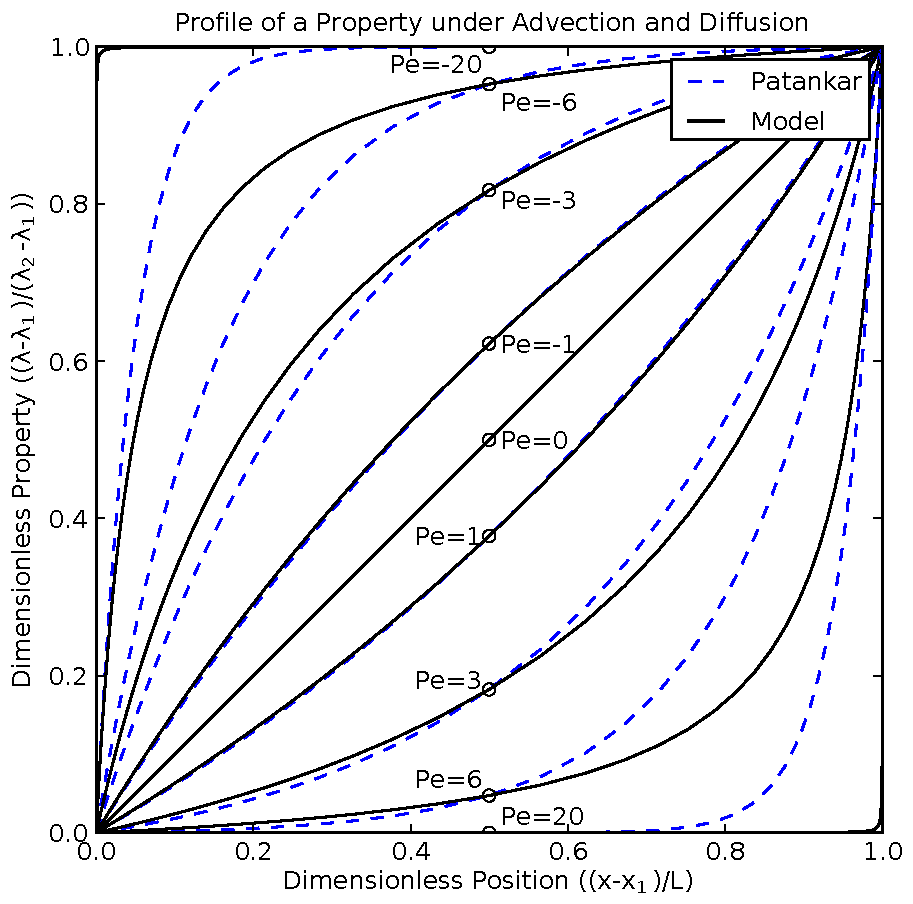
\includegraphics[width=0.75\linewidth]{3-AdvDiffProfile}%
  \caption[Profile of a property between regions due to advection and diffusion]{Center-to-center profile of a property between regions under advection and diffusion.  The model is equivalent to the Patankar's solution~\cite{Patankar1980} at the midplane ($\s{x} = \s{L}/2$)}%
  \label{fig:AdvDiffProfile}
\end{figure}

The previous evaluations are based on the condition that the flow rates of opposing transport equations are equal and opposite.  This is true at an interface between regions because the flow rate into one region is the rate out the other.  However, it is not necessarily the case across a region because the quantity may be stored within the region.  If we relax the previous assumption and provide the values of the driving property in the bulk of the region and at both boundaries, we can determine the rate of storage in a region:
\begin{equation}
  \label{eq:DiffusiveTransportStorage}
  \sum\dot{X} = \frac{\group{\s{gamma}[_neg] - \s{gamma}}\group{1 + e^{-\s{Pe}[_neg]/2}} + \group{\s{gamma}[_pos] - \s{gamma}}\group{1 + e^{\s{Pe}[_pos]/2}}}{\s{R}}
\end{equation}
If there is no advection, the rate of storage is proportional to the first-order approximation of the second derivative of the property over space:
\begin{equation}
  \sum\dot{X} = \frac{2}{\s{R}}\group{\s{gamma}[_neg] + \s{gamma}[_pos] - 2\s{gamma}}
\end{equation}

\autoref{tab:AdvDiff} shows the implications of \autoref{eq:DiffusiveTransportStorage}.  The third textual column and first graphic column indicate the rate of storage induced by positive or negative velocities and positive or negative property gradients under the condition of a linear property profile.  The fourth textual column and second graphic column indicate the concavity of the profile under the condition of no storage.  The curves are not to scale; \autoref{fig:AdvDiffProfile} gives the exact shape.  The boundary-to-boundary profile across a region must either match the first or second graphic column (and third or fourth textual column).  The center-to-center profile of a property must match the second graphic column---not the first since there is no storage at the interface between regions.

The first row of \autoref{tab:AdvDiff} indicates that if the property increases in the positive direction and the velocity is in the negative direction, either the conserved quantity is being removed from the region or the profile is concave up, or both.  If the gradient or the velocity is reversed, but not both, the quantity is stored instead or the concavity changes sign.  If both the gradient and the velocity are reversed, the storage regime and the concavity remain the same.  If the material flow is from higher to lower values of the property, the quantity is removed from the region; otherwise it is stored.  The concavity is always such that the gradient is lower on the side receiving the advection.

\begin{table}[hbt]
  \newcommand\C[1]{\multirow{2}*{#1}} % Hack to vertically align entries in a table
  \newcommand\G[1]{\C{\includegraphics[height=0.9cm]{#1}}} % Insert a graphic across two rows.
  \caption[Scenarios of \nname{1D} advection with diffusion]{Scenarios of \n{1D} advection with diffusion}%
  \label{tab:AdvDiff}%
  \begin{tabular}{ccccccccc}
    \toprule
    \textbf{Difference} & \C{$\land$} & \textbf{Velocity} & \C{$\Leftrightarrow$} & \textbf{Intake} & \C{$\lor$} & \textbf{Inflection} & \multicolumn{2}{c}{\textbf{Graphically:}} \\
    ($\Delta\s{gamma}$) & & (\s{phi}) & & ($\sum\dot{X}$) & & ($\Delta^2\s{gamma}$) & $\s{gamma}[_neg]\cdots\s{gamma}\cdots\s{gamma}[_pos]$ & or \\
    \midrule \addlinespace
    \C{$<0$} & & \C{$<0$} & & \C{$>0$} & & \C{$<0$} & \G{3-AdvDiffNegSlopeIn} & \G{3-AdvDiffNegSlopeDown} \\
    \\ \addlinespace
    \C{$<0$} & & \C{$>0$} & & \C{$<0$} & & \C{$>0$} & \G{3-AdvDiffNegSlopeOut} & \G{3-AdvDiffNegSlopeUp} \\
    \\ \addlinespace
    \C{$>0$} & & \C{$<0$} & & \C{$<0$} & & \C{$>0$} & \G{3-AdvDiffPosSlopeOut} & \G{3-AdvDiffPosSlopeUp} \\
    \\ \addlinespace
    \C{$>0$} & & \C{$>0$} & & \C{$>0$} & & \C{$<0$} & \G{3-AdvDiffPosSlopeIn} & \G{3-AdvDiffPosSlopeDown} \\
    \\ \addlinespace
    \bottomrule
  \end{tabular}%
\end{table}

The difference between the properties of adjacent regions is related to the flow rate between them by
\begin{equation}
  \s{gamma}_2 - \s{gamma}_1 = \dot{X}\group{\frac{\s{R}_1}{1 + e^{\s{Pe}/2}} + \frac{\s{R}_2}{1 + e^{-\s{Pe}/2}}}%
  \glsadd{_123}
\end{equation}
This follows from \autoref{eq:DiffusiveTransport3} (implemented for each region) and conservation of the transported quantity at the interface.  If the resistances are equal ($\s{R}_1 = \s{R}_2 = \s{R}$), then
\begin{equation}
  \label{eq:DiffusiveTransportTwoRegion}
  \s{R}\dot{X} = \s{gamma}_1 - \s{gamma}_2%
\end{equation}
which is typical diffusion.  This is applicable even if there is bulk material flow.  It confirms that the transport equation is a diffusion equation---only with upstream discretization so that advection can be properly determined.  Since the local gradient is affected by advection, the rate of diffusion is generally not proportional to the local gradient at the interface (given by \autoref{eq:MixingProfile}) but rather the average gradient between the centers of the regions.  Likewise, if there is no storage within a region along an axis and the P\'eclet numbers are equal at the boundaries, then
\begin{equation}
  \label{eq:DiffusiveTransportRegion}
  \s{R}\dot{X} = \s{gamma}[_neg] - \s{gamma}[_pos]
\end{equation}
where $\dot{X} = \dot{X}[_neg] = -\dot{X}[_pos]$.


\noindent\underline{\textbf{Discussion}}

The rate of advection is the product of the material flow rate and the amount of the quantity per unit of material (i.e., specific quantity).  In the case of material flow, this specific quantity is unity, since material is the quantity~\cite{Present1958}.  In the case of the translational advection, the specific quantity is velocity, the gradient of which also drives property.  For thermal advection, the specific quantity is temperature times specific entropy.  Temperature is the driving property for thermal diffusion, but specific entropy can be calculated from the temperature and concentration at the boundary.

\autoref{fig:AdvDiffFlow} shows the combined effects of advection and diffusion if the specific quantity is the same as the driving property for diffusion (e.g., translational advection).  The advection and diffusion are evaluated at the interface of two regions with the same resistances.  The property in the second region ($\s{gamma}_1\glsadd{_123}$) is arbitrarily five times the property in the first region ($\s{gamma}_2$).  The rate of diffusion is constant (in dimensionless units), as predicted by \autoref{eq:DiffusiveTransportTwoRegion}.  As advection is initially increased, the property at the interface becomes nearly the mean of the properties of the regions.  The actual rate of advection is quite different from the ideal rate given by the upstream scheme.  A correction must be applied because the property at the interface is not the property of the upstream region.  Here, that correction is called \emph{\n{irreversible advection}} because this part of advection has been affected by the irreversible process of diffusion.   As the magnitude of the P\'eclet number becomes large, the irreversible advection becomes negligible because the interface takes on the property of the upstream region.

\begin{figure}[htbp]
  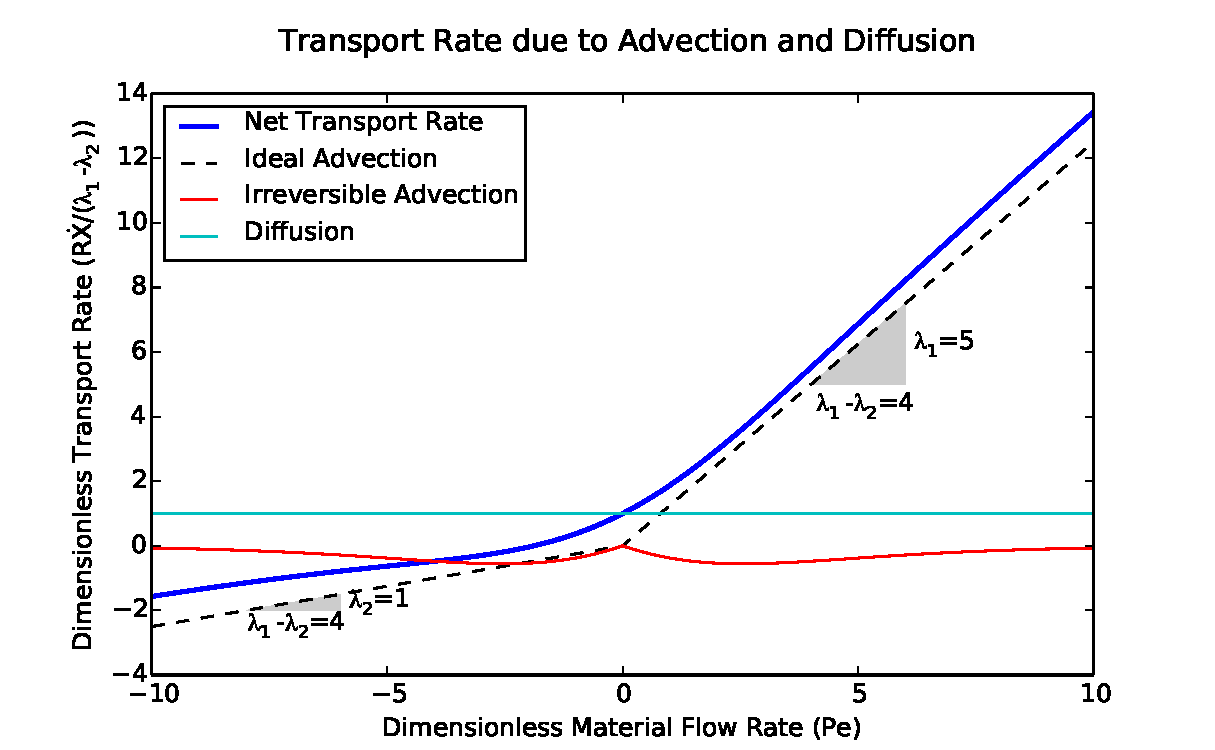
\includegraphics[width=0.9\linewidth]{3-AdvDiffFlow}%
  \caption{Transport rate of a conserved quantity under mixed advection and diffusion}%
  \label{fig:AdvDiffFlow}
\end{figure}

So far, we have evaluated the transport equations along one axis.  It is possible to implement \autoref{eq:DiffusiveTransport3} for all three dimensions simultaneously as long as the coordinate system is aligned with the principle axes of transport (Assumption \ref{itm:AssumeAligned} in the beginning of \autoref{sec:Transport}).   When the coordinate system is not aligned with the principle axes of transport, the model is subject to false diffusion like most methods of upstream discretization~\cite{Patankar1980}. 

Although the transport equation (\ref{eq:DiffusiveTransport3}) contains an exponential, it is not equivalent to the exponential scheme.  The exponential scheme is derived by \begin{inparaenum}[(1)]\item solving the advection\slash{}diffusion equation analytically for the profile of the driving property under the assumption of no storage and \item reintroducing the solution into the advection\slash{}diffusion equation without that original assumption\end{inparaenum}~\cite{Patankar1980, Majumdar2005}.  It results in a solution that is numerically singular unless there is advection.  The main argument against the exponential scheme---that it is computationally expensive---also applies to the transport equation used here.  However, the transport equation is used within a framework that \begin{inparaenum}[(1)]\item does not require a large number of regions for convergence and \item eliminates all nonlinear systems of equations\end{inparaenum}.  The argument may also be out of context now because it dates back to at least 1980~\cite{Patankar1980}, when computational resources were relatively limited.

As demonstrated in \autoref{sec:Exchange}, the traditional material derivative is the rate of diffusion.  This holds for transport as well.  The total rate of transport (\autoref{eq:Transport}) can be expanded with the rates of advection and diffusion from Equations \ref{eq:AdvectiveTransport} and \ref{eq:DiffusiveTransport2}:
\begin{equation}
  \dot{X}[_i]= \dot{N}[_i]\diffp{\s{X}}{\s{N}}[_i] + \Diff{\s{X}}{\s{t}}[_i]
\end{equation}
We will take this to be the positive side of the region so that the derivatives are in the positive direction and assume that the current is advective ($\dot{N} = -\s{phi}\s{A}\s{rho} =  -\s{phi}\partial\s{N}/\partial\s{x}$).  Then, dropping the subscripts,
\begin{equation}
  \dot{X} = -\s{phi}\diffp{\s{X}}{\s{x}} + \Diff{\s{X}}{\s{t}}
\end{equation}
Since the model uses a Eulerian perspective, the total transport rate \dot{X} is actually a partial derivative in the form of $\partial\s{X}/\partial\s{t}$.  After rearranging,
\begin{equation}
  \Diff{\s{X}}{\s{t}} = \diffp{\s{X}}{\s{t}} + \s{phi}\diffp{\s{X}}{\s{x}}
\end{equation}
Usually the scalar property in the material derivative is intensive (e.g., \s{gamma}, the driving property for diffusion).  Dividing by $\partial\s{X}/\partial\s{gamma}$,
\begin{equation}
  \Diff{\s{gamma}}{\s{t}} = \diffp{\s{gamma}}{\s{t}} + \s{phi}\diffp{\s{gamma}}{\s{x}}
\end{equation}
and generalizing to three dimensions,
\begin{equation}
  \Diff{\s{gamma}}{\s{t}} = \diffp{\s{gamma}}{\s{t}} + \boldsymbol{\s{phi}\cdot\nabla}\s{gamma}
\end{equation}
This is the definition of the material derivative~\cite{Bird2007}.

% Positive resistivity is characterized by irreversibility, damping, mixing, entropy production, and exergy destruction.  It corresponds to a real, stable situation where a distribution becomes uniform by exponential decay over time.  Zero resistivity is characterized by reversibility, zero damping, the maintenance of separation, and the absence of entropy production or exergy destruction.  It corresponds an ideal, marginally stable situation where distribution persists, because advection is perfectly balanced by transport around the region in the opposite direction.  Negative resistivity corresponds to a unstable situation where a distribution become less uniform by exponential growth over time.  It is physically impossible due to the second law of thermodynamics.


\subsection{Material Transport}
\label{sec:MaterialTransport}


As stated by James Clerk Maxwell, ``Mass transfer is due partly to the motion of translation and partly to that of agitation''~\cite{Burghardt2013}.  Here, the ``translation'' component of mass transfer is called material advection.  It is also called migration in the context of chemical engineering and drift in the context of solid state physics (\autoref{sec:Ohms}).  The ``agitation'' component is diffusion.  In accordance with Maxwell's statement, the total current into the region through boundary~\s{i} is the sum of the advective (``translation'') and diffusive (``agitation'') currents:
\begin{equation}
  \label{eq:MaterialTransport}
  \boxed{\dot{N}[_i]= \dot{N}\sub{_A}[_i] + \dot{N}\sub{_D}[_i]}
\end{equation}
This is simply \autoref{eq:Transport} where the transported quantity~(\s{X}) is material~(\s{N}).
% The total current can be written as
% \begin{equation}
%   \dot{N}[_i] = \frac{\s{k}\s{A}}{\s{zeta}\s{L}}\group{\s{rho}[_i] - \s{rho}}\group{1 + e^{\mp\s{zeta}\s{phi}[_perp]\s{L}/2\s{k}}} \pm \s{rho}[_i]\s{A}\group{\frac{\s{L}\s{beta}\dot{mPhi}\sub{_D}[_perp][_i]}{\s{k}\s{A}\group{1 + e^{\mp\s{beta}\s{M}\s{phi}[_perp]/2\s{k}\s{A}}}} + \s{phi}[_perp]}
% \end{equation}
% If there is zero net current and zero dynamic compressibility, then
% \begin{equation}
%   \s{rho} = \s{rho}[_i]\group{1 \pm \frac{\s{zeta}\s{L}}{\s{k}\group{1 + e^{\mp\s{zeta}\s{phi}[_perp]\s{L}/2\s{k}}} }\s{phi}[_perp]}
% \end{equation}


\subsubsection{Advection}

The general advection equation (\ref{eq:AdvectiveTransport}) reduces to an identity when the transported quantity~(\s{X}) is the amount of material~(\s{N}).  Instead, the amount of material in that equation is first replaced by the position into the region along the axis of transport.  Then, the partial derivative $\partial\s{X}/\partial\s{N}$ becomes $\partial\s{N}/\partial\s{x}$ or $\s{rho}\s{A}$.  The current \dot{N} becomes $\dot{x}$ or velocity directed into the region ($\pm\s{phi}$).  Therefore,
\begin{equation}
  \label{eq:MaterialAdvection}
  \boxed{\dot{N}\sub{_A}[_i] = \pm \s{phi}\sub{_perp}[_i]\s{rho}[_i]\s{A}[_i]}
\end{equation}
where the positive of $\pm$ is for the negative boundaries and the negative is for positive boundaries.  The subscript $\perp$ indicates the component of velocity normal to the boundary.  The value of the velocity will be established by \autoref{eq:NormalDiffusion}, but for now, it is considered known.



\subsubsection{Diffusion}
\label{sec:MaterialDiffusion}

The rate of material diffusion follows from Equations \ref{eq:DiffusiveTransport4} and \ref{eq:Peclet3}.  Material~(\s{N}) is the transported quantity~(\s{X}) and concentration~(\s{rho}) is the driving property~(\s{gamma}).
\begin{equation}
  \label{eq:MaterialDiffusion}
  \boxed{\s{zeta}\dot{N}\sub{_D}[_i] = \frac{\s{k}[_i]\s{A}[_i]}{\s{L}[_i]}\group{\s{rho}[_i] - \s{rho}}\group{1 + e^{\mp\s{zeta}\s{V}\s{phi}\sub{_perp}[_i]/2\s{k}[_i]\s{A}[_i]}}}
\end{equation}
where \dot{N}[_i] is the diffusive current into the region through boundary~\s{i}.  The volume~(\s{V}) is the volume of the phase.  However, the area~(\s{A}) is the cross-sectional area of the region along the axis of transport and \s{L}~is the length of the same.  The variable~\s{rho}[_i]~is the concentration or volumic amount of material at the boundary.   This concentration is not molar concentration or number concentration; it can be determined independently for each species.   The concentration in the region may be considered known, since it is a state of the material balance (\autoref{sec:BasicMaterialBalance}).  If a species is isochoric in a phase (e.g., liquid \n{H2O}), it will not diffuse.

The material resistivity, \s{zeta}, can be estimated from the generalized definition of resistivity (\autoref{eq:Resistivity}):
\begin{equation}
  \label{eq:MaterialResistivity}
  \boxed{\s{zeta} = \frac{3\s{tau}}{\s{lambda}^2}}
\end{equation}
The material resistivity is the reciprocal of self diffusivity, which is the ability of trace particles of a species to diffuse through other particles of the same species~\cite{Present1958}.  This is the essence of \autoref{eq:MaterialDiffusion}; it describes the rate of diffusion through an advected stream of particles of the same type.

The material transport equation is closely related to Fick's law\label{mark:FicksLaw}.  If we assume that the bulk velocity (and advective current) is zero along the axis of transport and the area factor (\s{k}[_i]) is unity, the rate of material diffusion (\autoref{eq:MaterialDiffusion}) reduces to
\begin{equation}
  \s{zeta}\dot{N}[_i] = 2\frac{\s{A}[_i]}{\s{L}[_i]}\group{\s{rho}[_i] - \s{rho}}
\end{equation}
If the concentration gradient is uniform, there is no material storage due to diffusion ($\dot{N}[_neg] = -\dot{N}[_pos] = \s{A}\s{J}$).  In that case, we can combine the negative- and positive-side equations as:
\begin{equation}
  \s{zeta}\s{J} = \frac{\s{rho}[_neg] - \s{rho}[_pos]}{\s{L}}
\end{equation}
Taking the limit as length goes to zero and generalizing to three dimensions,
\begin{equation}
  \s{zeta}\mathbf{\s{J}} = -\mathbf{\nabla}\s{rho}
\end{equation}
which is Fick's first law~\cite{Bird2002, Burghardt2013, Liggett1994, Wesselingh2000, Bockris2000, Taylor1993}.%\cite[p.~515]{Bird2002}, \cite[p.~426]{Liggett1994}

Fick's law also appears in other forms in the literature.  In theory, any intensive thermodynamic property could be used as long as it is sufficient to fix the thermodynamic state of the species given its temperature.  The choice affects the transport rate and thus the resistivity must be set properly, but it will not affect the equilibrium.  All of the intensive thermodynamic properties are uniform between two regions in thermodynamic equilibrium (aside from outside forces), and the equilibrium point is determined by the conservation equations (Sections~\ref{sec:BasicConservation} and \ref{sec:DetailedConservation}).

Since the species has constant specific mass, we can write Fick's law in terms of density~\cite{Burghardt2013, Bejan2006}:
\begin{equation}
  \s{m}\s{zeta}\timessep\s{J} = -\nabla\group{\s{mrho}}
\end{equation}
If the species exists in small amounts within an otherwise uniform mixture, the extensive volume (in $\s{rho} = \s{N}/\s{V}$) can be replaced by the total amount or mass of the phase.  For mole fractions, this is~\cite{Majumdar2005, Burghardt2013, Incropera2002, Taylor1993}
\begin{equation}
  \frac{\s{V}\s{zeta}}{\s{N}[_tot]}\timessep\s{J} \approx -\nabla\group{\s{N}/\s{N}[_tot]}
\end{equation}
where \s{N}~is the number of particles of the transported species and \s{N}[_tot]~is the total number of particles in the phase.  For mass fractions, we can write this as~\cite{Majumdar2005, Burghardt2013, Incropera2002, Taylor1993}
\begin{equation}
  \frac{\s{m}\s{V}\s{zeta}}{\s{M}[_tot]}\timessep\s{J} \approx -\nabla\group{\s{M}/\s{M}[_tot]}
\end{equation}
We can also write Fick's law in terms of partial pressure~\cite{Burghardt2013}:
\begin{equation}
  \diffp{\s{p}}{\s{rho}}[_T]\s{zeta}\timessep\s{J} = -\nabla\s{p}
\end{equation}
For ideal gases, this is
\begin{equation}
  \s{T}\s{zeta}\timessep\s{J} = -\nabla\s{p}
\end{equation}
Since the material resistivity is roughly the base resistivity factor divided by specific volume (see \autoref{eq:MaterialResistivity}), we can write this as (again, assuming ideal gas)
\begin{equation}
  \s{alpha}\timessep\s{J} = -\nabla\ln\s{p}
\end{equation}
For an isothermal ideal gas, \autoref{eq:GibbsFunction} implies that
\begin{equation}
  \label{eq:FicksLawGibbsIdealGas}
  \s{T}\s{alpha}\timessep\s{J} = -\nabla\s{g}
\end{equation}
Since \s{alpha}~is only dependent on temperature and fixed properties (specific mass and particle diameter), chemical potential (here, \s{g}) may be preferred as the driving property for material diffusion.  The magnitude of the diffusion rate in the previous forms of Fick's law is coupled to the concentration, which is affected over time by the diffusion itself (if storage is allowed).  We can also express Fick's law in terms of chemical potential for species that are not ideal gases~\cite{Matuszak2006}:
\begin{equation}
  \s{zeta}\group{\diffp{\s{g}}{\s{rho}}}\timessep\s{J} = -\nabla\s{g}
\end{equation}
If temperature is uniform, this is
\begin{equation}
  \frac{\s{zeta}}{\s{rho}}\diffp{\s{p}}{\s{rho}}[_T]\s{J} = -\nabla\s{g}
\end{equation}
If the species is an ideal gas, this again reduces to \autoref{eq:FicksLawGibbsIdealGas}.  The model uses concentration as the driving property for diffusion because the boundary pressure is needed for the momentum balance (\autoref{sec:TranslationalBalance}) and concentration is available as a dynamic property anyway.  Pressure is an explicit function of concentration as long as the species is compressible (\autoref{eq:VirialBerlin1}), but pressure cannot generally be expressed as a function of specific Gibbs energy (except in special cases).

% In the literature within the field of \np{PEMFC}~\cite{Weber-Review2004}, the transport process is often described with a viscous flow equation such as Darcy's law and $\n{n}[_spec] - 1$ repetitions of an equation consisting of momentum, Maxwell-Stefan diffusion, and Knudsen diffusion terms.  However, this approach is not rigorous in terms of energy.  Weber and Newman~\cite{Weber2005} note that the typical modeling approach, the dusty-gas model, can lead to a singular matrix.


\subsection{Normal Translational Advection and Nonequilibrium Compression}
\label{sec:NormalTransport}

In the previous section, we treated the normal component of velocity at a boundary ($\s{phi}\sub{_perp}[_i]$) as if it were known.  In this section, it is related to the velocity within the region by the effect of bulk or volume viscosity.  This entails a set of advection\slash{}diffusion equations for the normal component of translational momentum.

The normal force on boundary~\s{i} is due to the sum of the advective and diffusive forces:
\begin{equation}
  \label{eq:NormalForce}
  \dot{mPhi}\sub{_perp}[_i] = \dot{mPhi}\sub{_A}[_perp][_i] + \dot{mPhi}\sub{_D}[_perp][_i]
\end{equation}
This follows the form of \autoref{eq:Transport} where the transported quantity~(\s{X}) is the normal component of translational momentum~(\s{mPhi}).  The advective component is often called dynamic pressure (or force in this case) and the diffusive component may be called nonequilibrium pressure~\cite{Meier2005}.  Thermodynamic pressure is excluded here, but it is included in the translational momentum balance (\autoref{eq:TranslationalBalance}).


\subsubsection{Advection}
\label{sec:NormalAdvection}

The advective normal force follows from \autoref{eq:AdvectiveTransport}.
\begin{equation}
  \label{eq:NormalAdvection}
  \dot{mPhi}\sub{_A}[_perp][_i] = \dot{N}[_i]\s{m}\s{phi}\sub{_perp}[_i]
\end{equation}
where $\s{phi}\sub{_perp}[_i]$~is the normal velocity at boundary~\s{i}.  Since this equation applies to each configuration separately, the specific mass at the boundary (\s{m}[_i]) is the same as the specific mass in the region~(\s{m}) and the subscript is not necessary.  The current (\dot{N}[_i]) includes advective and diffusive parts according to \autoref{eq:MaterialTransport}.


Using Equations \ref{eq:MaterialTransport} and \ref{eq:MaterialAdvection}, the advective normal force can be expanded as
\begin{equation}
  \label{eq:NormalAdvection2}
  \dot{mPhi}\sub{_A}[_perp][_i] = \s{m}\dot{N}\sub{_D}[_i]\s{phi}\sub{_perp}[_i] \pm \s{m}\s{rho}[_i]\s{A}[_i]\s{phi}\sub{_perp}[_i]^2
\end{equation}
where \s{x}~is the position along the axis of transport.  The second term on the right side is closely related to the dynamic pressure\label{mark:DynamicPressure} ($\s{m}\s{rho}\s{phi}^2/2$) usually expressed in \np{PDE}.  However, the essence of dynamic pressure---the advection of translational momentum---is implemented directly instead of using a discrete approximation to the traditional \np{PDE}.  Assuming that the specific mass and concentration are constant, the derivative of the traditional dynamic pressure is $\s{m}\s{rho}\s{phi}\partial\s{phi}$.  The force that results over a distance $\mathrm{d}\s{x}$ is $\s{M}\s{phi}\partial\s{phi}/\partial\s{x}$.  The first-order discrete approximation is $\s{M}\s{phi}\Delta\s{phi}/\s{L}$; its implementation would yield a boundary force of $\pm\s{m}\s{rho}\s{A}\s{phi}[_perp]\s{phi}\sub{_perp}[_i]$ in the nomenclature of \autoref{eq:NormalAdvection2}.  This is only an approximation to the force due to material advection.  It does not guarantee conservation of momentum at the boundary, since adjacent regions may have different normal velocities (\s{phi}[_perp]).  This is troubling because the lack of conservation can lead to artificial instabilities.  The actual force---the one used in the model---involves the product of density, advective current, and velocity precisely at the interface (second term on the right side of \autoref{eq:NormalAdvection2}).


\subsubsection{Diffusion}
\label{sec:NormalDiffusion}

The diffusive normal force follows from \autoref{eq:DiffusiveTransport4} with the component of velocity normal to the boundary (\s{phi}[_perp]) as the diffusion-driving property~(\s{gamma}):
\begin{equation}
  \label{eq:NormalDiffusion}
  \boxed{\s{beta}\dot{mPhi}\sub{_D}[_perp][_i] = \frac{2\s{k}[_i]\s{A}[_i]}{\s{L}[_i]}\Group{\s{phi}\sub{_perp}[_i] - \s{phi}[_perp]\frac{\s{V}}{\s{V}[_tot]}}}
\end{equation}
This is the force due to nonequilibrium compression.  The form of the equation departs from the general equation (\ref{eq:DiffusiveTransport4}) in two ways, which will be explained.

The first departure from \autoref{eq:DiffusiveTransport4} is that the porosity, $\s{V}/\s{V}[_tot]$, has been applied to the velocity in the region to account for the presence of other phases.  If multiple phases are present in the region, only part of the boundary is open to material transport in any one of the phases.  Yet the material advection equation (\ref{eq:MaterialAdvection}) assumes that the velocity is uniform over the boundary.  The porosity is an attempt to account for this inaccuracy.  The fraction of open area at the boundary (e.g., areal porosity) is assumed to be the fraction of open volume in the region (e.g., volumetric porosity).  The porosity cannot be introduced directly in the material advection equation because neighboring regions may have different volume fractions.  If it were, material conservation would be violated at the boundary.  By placing the porosity in \autoref{eq:NormalDiffusion}, the neighboring regions must agree on the fraction of open area at their common boundary.

The second departure is that no upstream discretization has been applied in \autoref{eq:NormalDiffusion}.  The velocity at the boundary is assumed to be zero for the sake of calculating the P\'eclet number at the boundary (\autoref{eq:Peclet3}).  A nonzero P\'eclet number would imply that the velocity at the boundary anticipates the propagation of the velocity property itself from the center of the region to the boundary.  This seems to be a violation of physics.


The variable~\s{beta} represents the \emph{\n{dynamic compressibility}} which describes the extent to which a non-equilibrium normal force causes or requires transient compression.  It can be estimated from the generalized definition of resistivity (\autoref{eq:Resistivity}):
\begin{equation}
  \label{eq:DynamicCompressibility}
  \boxed{\s{beta} = \frac{3\s{tau}}{\s{lambda}^2\s{rho}\s{m}}}
\end{equation}
Dynamic compressibility is the reciprocal of bulk viscosity as a dynamic (rather than kinematic) viscosity.  Although bulk viscosity differs from shear viscosity~\cite{Karim1952, Schetz1996, Rah1999, Liggett1994}, % \cite[p.~25]{Liggett1994}
the same initial estimate is used.  Dynamic compressibility is different from compressibility, which is $-\group{\partial\s{v}/\partial\s{p}}/\s{v}$.


\subsection{Transverse Translational Advection and Friction}
\label{sec:TransverseTransport}

The force on boundary~\s{i} transverse to the surface is due to the sum of the advective and diffusive forces:
\begin{equation}
  \label{eq:TransverseForce}
  \dot{mPhi}\sub{_para}[_i] = \dot{mPhi}\sub{_A}[_para][_i] + \dot{mPhi}\sub{_D}[_para][_i]
\end{equation}
This follows the form of \autoref{eq:Transport} where the transported quantity~(\s{X}) is a component of translational momentum transverse to the boundary (\s{mPhi}[_para]).  This equation is implemented twice---once for each transverse direction.


\subsubsection{Advection}

Translational momentum is advected according to the generalized advective transport equation (\ref{eq:AdvectiveTransport}).  In terms of the present variables, this is
\begin{equation}
  \label{eq:TransverseAdvection}
  \dot{mPhi}\sub{_A}[_para][ ][_i] = \dot{N}[_i]\s{m}\s{phi}\sub{_para}[ ][_i]
\end{equation}
where $\s{phi}\sub{_para}[ ][_i]$ is a component of velocity transverse to boundary~\s{i}.  Since this equation applies to each configuration separately, the specific mass at the boundary (\s{m}[_i]) is the same as the specific mass in the region~(\s{m}) and the subscript is not necessary.  The current (\dot{N}[_i]) includes advective and diffusive parts according to \autoref{eq:MaterialTransport}.


\subsubsection{Diffusion}

The friction or shear force along a boundary follows the generalized diffusive transport equation (\ref{eq:DiffusiveTransport4}) with an adjustment factor.  The  driving property is a transverse component of velocity (\s{phi}[_para]) aligned with the shear force.
\begin{equation}
  \label{eq:ShearForce}
  \boxed{\s{eta}\dot{mPhi}\sub{_D}[_para][ ]{_i}\sup{^prime} = \frac{\s{Nu}[_Phi]\s{k}[_i]\s{A}[_i]}{\s{L}[_i]}\group{\s{phi}\sub{_para}[ ]{_i} - \s{phi}[_para]}\group{1 + e^{\mp\s{eta}\s{M}\s{phi}\sub{_perp}[_i]/2\s{k}[_i]\s{A}[_i]}}}
\end{equation}
where $\dot{mPhi}\sub{_D}[_para][ ]{_i}\sup{^prime}$ is the shear force.  The reason for the prime superscript will be discussed below.  The boundary velocity ($\s{phi}\sub{_para}[ ][_i]$) is an effective velocity.  Its usage does not imply that the velocity is uniform over the boundary (which would generally lead to discontinuities in the velocity at the edges of the boundary).  Unlike the normal diffusive force (\autoref{eq:NormalDiffusion}), the shear force uses upstream discretization.  The associated P\'eclet number is based on the normal component of velocity at the boundary ($\s{phi}\sub{_perp}[_i]$).

The fluidity, \s{eta}, can be estimated from the generalized definition of resistivity (\autoref{eq:Resistivity}):
\begin{equation}
  \label{eq:Fluidity}
  \boxed{\s{eta} = \frac{3\s{tau}}{\s{lambda}^2\s{rho}\s{m}}}
\end{equation}
Fluidity is the reciprocal of shear viscosity as a dynamic (rather than kinematic) viscosity.  If two adjacent regions have zero fluidity~(\s{eta}), the parallel components of their velocities are equal and the number of states is reduced by two.  Translational momentum will flow between the regions without loss.

The additional variable~\s{Nu}[_Phi] is the shear shape factor or the \emph{\n{translational Nusselt number}}---the analog of the traditional or thermal Nusselt number for the diffusion of translational momentum.  It allows the shear force equation (\ref{eq:ShearForce}) to be used at relatively coarse levels of discretization.  It is defined as the ratio of the average inward velocity gradient along the perimeter divided by the difference between the boundary velocity and the bulk velocity over the distance from the boundary to the center of the region:
\begin{equation}
  \label{eq:TranslationalNusselt}
  \s{Nu}[_Phi] \equiv \left.\diffp{\s{phi}[_para]}{\s{x}}[_i]\middle/2\frac{\s{phi}\sub{_para}[ ][_i] - \s{phi}[_para]}{\s{L}[_x]}\right.
\end{equation}
\autoref{tab:TranslationalNusselt} summarizes the shape factor or the translational Nusselt number given two assumptions: \begin{inparaenum}[(1)]\item the material concentration is uniform and \item the boundary velocities are uniform around the perimeter\end{inparaenum}.  The first assumption implies that the bulk, mass-average velocity is equal to the volume-average velocity.  The shape factor is one in a \nfirst{2D} case (where no force is applied the third dimension, e.g., its length is infinite) with a linear velocity profile.  The velocity changes from the boundary velocity to the bulk velocity (solid blue vertical line) in half of the distance between the boundaries.  The shape factor is two in a \nfirst{2D} case with a piecewise linear velocity profile.  Then, the velocity changes from the boundary velocity to the bulk velocity in one fourth of the distance between the boundaries.  The shape factor is three in a \nfirst{3D} case with a piecewise linear velocity profile because the volume of a pyramid is one third the product of its base area and height.  The shape factor is four if the flow is fully developed and laminar (Hagen-Poiseuille flow, discussed below).  If the flow is turbulent, the shape factor is greater than four; the velocity gradient at the wall is greater than for laminar flow.

\begin{table}[hbt]
  \newcommand\C[1]{\multirow{4}*{#1}} % Hack to vertically align entries in a table
  \newcommand\G[1]{\C{\includegraphics[height=2cm]{#1}}} % Insert a graphic across multiple rows.
  \caption{Values of the translational Nusselt number}%
  \label{tab:TranslationalNusselt}%
  \begin{tabular}{cccl}
    \toprule
    \textbf{Shape factor} & \multirow{2}*{\textbf{Profile}} & \textbf{Number of} & \multirow{2}*{\textbf{Description}} \\
    (\s{Nu}[_Phi]) &  & \textbf{dimensions} &  \\
    \midrule \addlinespace
    \C{1} & \G{3-ShapeFactorCouette} & \C{2} & \C{Couette flow (linear)} \\
    \\ \\ \\\addlinespace
    \C{2} & \G{3-ShapeFactorPiecewise2D} & \C{2} & \C{Piecewise linear (triangle)} \\
    \\ \\ \\\addlinespace
    \C{3} & \G{3-ShapeFactorPiecewise3D} & \C{3} & \C{Piecewise linear (pyramid)} \\
    \\ \\ \\\addlinespace
    \C{4} & \G{3-ShapeFactorLaminar} & \C{3} & \C{Laminar fully developed (parabola)} \\
    \\ \\ \\\addlinespace
    \C{$>4$} & \G{3-ShapeFactorTurbulent} & \C{3} & \C{Turbulent (higher order)} \\
    \\ \\ \\\addlinespace
    \bottomrule
  \end{tabular}%
\end{table}

The model does not directly use the shear force equation (\ref{eq:ShearForce}) because the forces apply torques and the model is based on the assumption that rotational momentum is not stored (see \autoref{sec:RotationalConservation}).  This is the reason for the prime superscript in the shear force equation (\ref{eq:ShearForce}).  The conservation of rotational momentum (\autoref{eq:RotationalConservationX}) gives one of the four equations required for the four boundaries around the perimeter of the region along the x~axis.  The first of the remaining three equations requires that the total force in the y direction is the force determined by the y-direction shear force equations:
\begin{equation}
  \boxed{\dot{mPhi}\sub{_y}[_neg][_z] + \dot{mPhi}\sub{_y}[_pos][_z] = \dot{mPhi}\sub{_y}[_neg][_z]\sup{^prime} + \dot{mPhi}\sub{_y}[_pos][_z]\sup{^prime}}
\end{equation}
Similarly in the z direction:
\begin{equation}
  \boxed{\dot{mPhi}\sub{_z}[_neg][_y] + \dot{mPhi}\sub{_z}[_pos][_y] = \dot{mPhi}\sub{_z}[_neg][_y]\sup{^prime} + \dot{mPhi}\sub{_z}[_pos][_y]\sup{^prime}}
\end{equation}
The final equation requires that the torque applied to the y boundaries opposes the torque applied to the z boundaries to the same extent calculated by the shear force equations:
\begin{equation}
  \boxed{\group{\dot{mPhi}\sub{_z}[_neg][_y] - \dot{mPhi}\sub{_z}[_pos][_y]}\s{L}[_z] + \group{\dot{mPhi}\sub{_y}[_neg][_z] - \dot{mPhi}\sub{_y}[_pos][_z]}\s{L}[_y] =  \group{\dot{mPhi}\sub{_z}[_neg][_y]\sup{^prime} - \dot{mPhi}\sub{_z}[_pos][_y]\sup{^prime}}\s{L}[_z] + \group{\dot{mPhi}\sub{_y}[_neg][_z]\sup{^prime} - \dot{mPhi}\sub{_y}[_pos][_z]\sup{^prime}}\s{L}[_y]}
\end{equation}
Similar equations apply to the perimeters around the y and z axes.  The translational advection equation (\ref{eq:TransverseAdvection}) is applied directly; we assume that it interacts with the center of the region and produces no torque.

% If we use the shear force equation (\ref{eq:ShearForce}) and assume that the cross-wise components of velocity are zero, we can write the three new shear force equations as
% \begin{subequations}
%   \begin{equation}
%     \label{eq:ShearForceY}
%     \dot{mPhi}\sub{_y}[_neg][_z] + \dot{mPhi}\sub{_y}[_pos][_z] = \frac{2\s{Nu}[_Phi]\s{A}[_y]}{\s{eta}\s{L}[_y]}\group{\s{phi}\sub{_y}[_neg][_z] + \s{phi}\sub{_y}[_pos][_z] - 2\s{phi}[_y]}
%   \end{equation}
%   \begin{equation}
%     \label{eq:ShearForceZ}
%     \dot{mPhi}\sub{_z}[_neg][_y] + \dot{mPhi}\sub{_z}[_pos][_y] = \frac{2\s{Nu}[_Phi]\s{A}[_z]}{\s{eta}\s{L}[_z]}\group{\s{phi}\sub{_z}[_neg][_y] + \s{phi}\sub{_z}[_pos][_y] - 2\s{phi}[_z]}
%   \end{equation}
%   \begin{equation}
%     \label{eq:ShearForceCounter}
%     \group{\dot{mPhi}\sub{_z}[_neg][_y] - \dot{mPhi}\sub{_z}[_pos][_y]}\s{L}[_y] + \group{\dot{mPhi}\sub{_y}[_neg][_z] - \dot{mPhi}\sub{_y}[_pos][_z]}\s{L}[_z] = \frac{2\s{Nu}[_Phi]}{\s{eta}}\Group{\group{\s{phi}\sub{_z}[_neg][_y] - \s{phi}\sub{_z}[_pos][_y]}\s{A}[_y] + \group{\s{phi}\sub{_y}[_neg][_z] - \s{phi}\sub{_y}[_pos][_z]}\s{A}[_z]}
%   \end{equation}
% \end{subequations}
% Equations~\ref{eq:ShearForceY} and \ref{eq:ShearForceZ} involve second-order differences, but \autoref{eq:ShearForceCounter} only involves first-order differences.

In three dimensions, this method involves a system of twelve equations which can be solved for the twelve shear forces (two for each of six boundaries).  The shear forces in the x direction are:
\begin{subequations}
  \label{eq:ForceMap}
  \begin{align}
    4\dot{mPhi}\sub{_y}[_neg][_x] &= 3\dot{mPhi}\sub{_y}[_neg][_x]\sup{^prime} + \dot{mPhi}\sub{_y}[_pos][_x]\sup{^prime} + \frac{\s{L}[_x]}{\s{L}[_y]}\group{\dot{mPhi}\sub{_x}[_neg][_y]\sup{^prime} - \dot{mPhi}\sub{_x}[_pos][_y]\sup{^prime}} \\
    4\dot{mPhi}\sub{_y}[_pos][_x] &= 3\dot{mPhi}\sub{_y}[_pos][_x]\sup{^prime} + \dot{mPhi}\sub{_y}[_neg][_x]\sup{^prime} + \frac{\s{L}[_x]}{\s{L}[_y]}\group{\dot{mPhi}\sub{_x}[_pos][_y]\sup{^prime} - \dot{mPhi}\sub{_x}[_neg][_y]\sup{^prime}} \\
    4\dot{mPhi}\sub{_z}[_neg][_x] &= 3\dot{mPhi}\sub{_z}[_neg][_x]\sup{^prime} + \dot{mPhi}\sub{_z}[_pos][_x]\sup{^prime} + \frac{\s{L}[_x]}{\s{L}[_z]}\group{\dot{mPhi}\sub{_x}[_neg][_z]\sup{^prime} - \dot{mPhi}\sub{_x}[_pos][_z]\sup{^prime}} \\
    4\dot{mPhi}\sub{_z}[_pos][_x] &= 3\dot{mPhi}\sub{_z}[_neg][_x]\sup{^prime} + \dot{mPhi}\sub{_z}[_neg][_x]\sup{^prime} + \frac{\s{L}[_x]}{\s{L}[_z]}\group{\dot{mPhi}\sub{_x}[_pos][_z]\sup{^prime} - \dot{mPhi}\sub{_x}[_neg][_z]\sup{^prime}}
  \end{align}
\end{subequations}
Thus, the force applied to a boundary is three fourths of the force calculated directly from \autoref{eq:ShearForce} plus one fourth of the calculated force on the opposing boundary minus the calculated forces on the perpendicular faces which are scaled to oppose the torques implied by \autoref{eq:ShearForce}.  This is shown graphically in \autoref{fig:ForceMap} for a cubic region ($\s{L}[_x] = \s{L}[_y] = \s{L}[_z]$).  The sum of the applied forces is equal to the forces calculated directly from \autoref{eq:ShearForce}:
\begin{equation}
  \dot{mPhi}\sub{_y}[_neg][_x] + \dot{mPhi}\sub{_y}[_pos][_x] + \dot{mPhi}\sub{_z}[_neg][_x] + \dot{mPhi}\sub{_z}[_pos][_x] = \dot{mPhi}\sub{_y}[_neg][_x]\sup{^prime} + \dot{mPhi}\sub{_y}[_pos][_x]\sup{^prime} + \dot{mPhi}\sub{_z}[_neg][_x]\sup{^prime} + \dot{mPhi}\sub{_z}[_pos][_x]\sup{^prime}
\end{equation}
Similar equations apply around the y and z axes.
% Solved in ShearForces.cdf

\begin{figure}[htbp]
  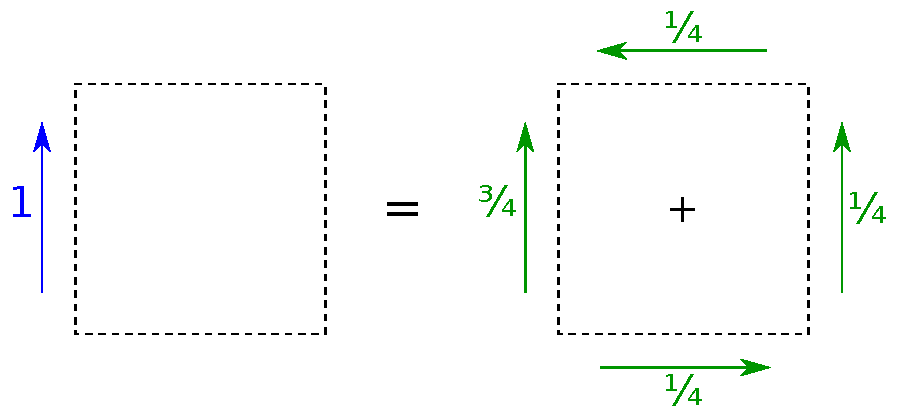
\includegraphics[width=0.6\linewidth]{3-ForceMap}%
  \caption[Weighting scheme to achieve zero torque]{Weighting scheme to achieve zero torque.  The left side is the force applied to a boundary and the right side contains the forces calculated from \autoref{eq:ShearForce}}%
  \label{fig:ForceMap}
\end{figure}

This mapping of shear velocities to shear forces is different from Stokes' viscous deformation law~\cite{Majumdar2005}\label{mark:Deformation}.  Both methods impose zero torque (i.e., conservation of rotational momentum without storage), but a discrete implementation of Stokes' viscous deformation law would do so at every boundary.  This is not necessary; the boundaries have zero thickness and thus zero moment.  However, there is a moment from the boundaries to the center of the control volumes.  Thus, the model imposes zero torque on each control volume as a whole.

If the normal bulk velocity is zero, the shear force equation reduces to
\begin{equation}
  \dot{mPhi}\sub{_D}[_para][ ]{_i} = \frac{2\s{Nu}\sub{_Phi}[_i]\s{A}[_i]}{\s{eta}\s{L}[_i]}\group{\s{phi}\sub{_para}[ ]{_i} - \s{phi}[_para]}
\end{equation}
If the velocity gradient is uniform ($\s{Nu}[_Phi] = 1$), translational momentum is not stored due to diffusion ($\dot{mPhi}\sub{_D}[_para][ ][_neg] = -\dot{mPhi}\sub{_D}[_para][ ][_pos] = \s{A}\s{J}$).  In that case, we can combine the negative- and positive-side equations as\label{mark:Couette}:
\begin{equation}
  \s{J} = \frac{\s{phi}\sub{_para}[ ][_neg] - \s{phi}\sub{_para}[ ][_pos]}{\s{eta}\s{L}}
\end{equation}
This maps directly to the actual shear stress if there is no shear force from the other two boundaries along the perimeter.  It is the first-order approximation to Newton's law of viscous shear, which describes Couette flow~\cite{Lienhard2006}. %[p. 281]

The shear force equation results in the expected pressure loss for fully-developed laminar pipe flow (i.e., Hagen-Poiseuille flow)\label{mark:Poiseuille}.  Suppose that material is flowing in the x direction with velocity~\s{phi} through a region with dimensions~\s{L}[_x], \s{L}[_y], and \s{L}[_z].  The bulk velocities in the y and z  directions are zero and the x-direction velocity is zero at the y and z boundaries (i.e., no slip).  According to \autoref{eq:ShearForce}, the total shear force on the y and z boundaries is
\begin{equation}
  \dot{mPhi}[_tot] = -\frac{4\s{Nu}[_Phi]\s{L}[_x]\s{phi}}{\s{eta}}\group{\frac{\s{L}[_z]}{\s{L}[_y]} + \frac{\s{L}[_y]}{\s{L}[_z]}}
\end{equation}
If the flow is fully developed, steady, and laminar, $\s{Nu}[_Phi] = 4$.  We may write the equation in terms of the hydraulic diameter ($\s{D} \equiv 4\s{A}/\s{P}$)~\cite{Incropera2002}, which is $2\s{L}[_y]\s{L}[_z]/(\s{L}[_y] + \s{L}[_z])$ in this case.  If there are no other forces the shear force must be balanced by the normal force ($\s{L}[_y]\s{L}[_z]\Delta\s{p} = \dot{mPhi}[_tot]$; see the conservation of translational momentum in \autoref{sec:BasicTranslationalBalance}).  With these assumptions and substitutions,
\begin{equation}
  \Delta\s{p} = \frac{64\s{L}[_x]\s{phi}}{\s{eta}\s{D}^2}\group{\frac{2}{2 + \frac{\s{L}[_y]}{\s{L}[_z]} + \frac{\s{L}[_z]}{\s{L}[_y]}} - 1}
\end{equation}
If we assume that the cross section is square ($\s{L}[_y] = \s{L}[_z]$), this reduces to
\begin{equation}
  \Delta\s{p} = -\frac{32\s{L}[_x]\s{phi}}{\s{eta}\s{D}^2}
\end{equation}
which is Poiseuille's law.  It can be derived by integrating a differential representation of the shear force equation (\ref{eq:ShearForce}) with a translational Nusselt number of one under the assumption of uniform pressure and a no-slip condition around a circular pipe~\cite{Cengel2006}.  This implies that the model should give the same result without the shear shape factor (i.e., $\s{Nu}[_Phi] = 1$) under a sufficiently fine level of discretization.  As mentioned previously, the shear shape factor is introduced to allow much coarser levels of discretization, and here it is set to four.

The model cannot directly describe turbulence\label{mark:Turbulence} because it assumes that the rotational momentum is zero.  This implies that eddies are not generated or are dissipated immediately upon generation.  A full description would require equations for the storage, exchange, and transport of rotational momentum.  Instead, correlations for turbulent flow are cast into the shear shape factor, which may vary with time and depend on the conditions.  This approach is consistent with the statement by Patankar~\cite{Patankar1980}: %[p.~15]
``From a computational viewpoint, a turbulent flow within this framework is equivalent to a laminar flow with a rather complicated prescription of viscosity.''  The only difference in this respect is that the present model has an adjustment factor (\s{Nu}[_Phi]) which is separate from the fluidity (or reciprocal of viscosity).

If rotational momentum were included, it is plausible that at a sufficiently fine level of discretization the model could describe turbulence.  In reality, shear force generates eddies that drive material towards alternating boundaries around the perimeter---normal to the direction of primary flow.  This effect would decrease the advection-adjusted length between the bulk velocity and a boundary (see \autoref{eq:ShearForce}) and increase the shear force for any velocity difference.  The criteria for the effect is that a sufficient amount of translational momentum is diverted from the direction of primary flow towards a boundary (e.g., by surface roughness).  It is a positive feedback mechanism; as more translational momentum is diverted towards the boundary due to shear force, more shear force is produced, until the translational momentum in the primary direction is sufficiently depleted.  Suppose we let \s{omega} be the diversion angle at the onset of the positive feedback.  Then, the P\'eclet number in the applicable shear force equation is
\begin{equation}
  \s{Pe} = \frac{\s{eta}\s{M}\s{phi}\sin\s{omega}}{\s{k}\s{A}}
\end{equation}
where \s{phi}~is the bulk velocity in the primary direction.  If we assume that the cross section is square, the hydraulic diameter is the length of a side ($\s{D} = \s{L} = \s{V}/\s{A}$).  If we also assume that the area factor is one ($\s{k} = 1$), then
\begin{equation}
  \s{Pe} = \s{mrho}\s{eta}\s{D}\s{phi}\sin\s{omega}
\end{equation}
The factor $\s{mrho}\s{eta}\s{D}\s{phi}$ is the Reynolds number; therefore
\begin{equation}
  \s{Pe} = \s{Re}\sin\s{omega}
\end{equation}
The discretization scheme becomes nearly saturated (as the upwind scheme) at roughly $\s{Pe} = 10$ (see \autoref{fig:AdvDiffRegion}) whereas turbulence begins at roughly 2300~\cite{Cengel2006}.  If we assume that turbulence corresponds to saturation of the discretization scheme, $\s{omega} \approx 0.25^\circ$.


\subsection{Thermal Advection and Conduction}
\label{sec:ThermalTransport}


As mentioned in \autoref{sec:BasicEnergyBalance}, the thermal transfer through an interface \s{i}~is divided into advective and diffusive parts:
\begin{equation}
  \label{eq:ThermalTransport}
  \dot{Q}[_i] = \dot{Q}\sub{_A}[_i] + \dot{Q}\sub{_D}[_i]
\end{equation}
This follows the form of \autoref{eq:Transport} where the transported quantity~(\s{X}) is heat~(\s{Q}).  This does not imply that heat is treated as a thermodynamic property; it only appears in a flow rate or a partial derivative, since it is process-dependent.  The advective term includes a component of enthalpy.  The diffusive part is thermal conduction.

As mentioned in \autoref{sec:BasicEnergyBalance}, thermal convection is the serial combination of thermal conduction and the advection of energy.  This is shown in \autoref{fig:ThermalConvection}.  The thermal conduction typically occurs between a solid and a fluid, which is an exchange process in the model.  However, we may assume that the thermal exchange occurs in a region of negligible thickness centered at the solid-fluid interface and that the fluid has the same temperature of the fluid there (i.e, no contact resistance).  Then, thermal convection is governed by two remaining processes in series: \begin{inparaenum}[(1)]\item thermal conduction between the fluid in the negligibly thin region and the fluid in a larger neighboring region and \item the advection through the larger region in the direction transverse to the boundary\end{inparaenum}.

\begin{figure}[htbp]
  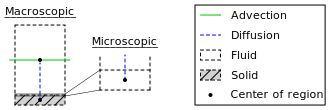
\includegraphics[width=0.65\linewidth]{3-ThermalConvection}%
  \caption{Thermal convection in the model}%
  \label{fig:ThermalConvection}
\end{figure}


\subsubsection{Advection}

Energy is advected according to the generalized advective transport equation (\ref{eq:AdvectiveTransport}) where the property $\partial\s{X}/\partial\s{N}$ is $\s{s}\s{T}$:
\begin{equation}
  \label{eq:ThermalAdvectiveTransport}
  \dot{Q}\sub{_A}[ ][_i] = \dot{N}[_i]\group{\s{s}\s{T}}[_i]
\end{equation}
The factor $(\s{s}\s{T})\sub{_i}$, combined with \s{g}[_i] of the material term, comprises the enthalpy associated with the material flow (as discussed in Sections~\ref{sec:BasicEnergyBalance} and \ref{sec:ThermalAdvectiveExchange}).  That factor is analogous to $\s{m}\s{phi}[_i]$ in the equations for translational advection (\ref{eq:NormalAdvection} and \ref{eq:TransverseAdvection}).  However, whereas the specific mass at the boundary is equal to the specific mass in the region, the specific entropy at the boundary is not generally equal to the specific entropy in the region ($\s{m}[_i] = \s{m}$, but $\s{s}[_i] \ne \s{s}$).  The temperature~(\s{T}) is the diffusion-driving property, like the velocity~(\s{phi}).


\subsubsection{Diffusion}

Like friction, thermal conduction or diffusion follows the form of the general transport equation (\ref{eq:DiffusiveTransport3}) with an adjustment factor (here, \s{Nu}[_Q]):
\begin{equation}
  \label{eq:ThermalDiffusiveTransport}
  \boxed{\s{theta}\dot{Q}[_i] = \frac{\s{Nu}[_Q]\s{k}[_i]\s{A}[_i]}{\s{L}[_i]}\group{\s{T}[_i] - \s{T}}\group{1 + e^{\mp\s{theta}\s{C}[_v]\s{phi}\sub{_perp}[_i]/2\s{k}[_i]\s{A}[_i]}}}
\end{equation}
The variable~\s{T}[_i] is the temperature at boundary~\s{i}, and $\dot{Q}[_i]$~is the rate of thermal conduction into the region through the boundary.  The temperature in the region~(\s{T}) may be considered known, since it is a state of the energy balance (\autoref{sec:BasicEnergyBalance}).

The thermal resistivity, \s{theta}, can be estimated from the generalized definition of resistivity (\autoref{eq:Resistivity}).
\begin{equation}
  \label{eq:ThermalResistivity}
  \boxed{\s{theta} = \frac{3\s{tau}}{\s{lambda}^2\s{rho}\s{c}[_v]}}
\end{equation}
where the partial derivative is taken at constant volume because the regions have fixed volume.  This equation matches the thermal conductivity given by Present~\cite{Present1958}, noting that thermal conductivity is the reciprocal of thermal resistivity~\cite{Incropera2002}.

The adjustment factor~\s{Nu}[_Q] is the traditional (thermal) Nusselt number\label{mark:Nusselt}.   It allows the thermal conduction equation to be used at relatively coarse levels of discretization.  It is the ratio of the average inward temperature gradient along the perimeter divided by the difference between the boundary temperature and the bulk temperature over the distance from the boundary to the center of the region:
\begin{equation}
  \label{eq:ThermalNusselt}
  \s{Nu}[_Q] \equiv \left.\diffp{\s{T}}{\s{x}}[_i]\middle/2\frac{\s{T}[_i] - \s{T}}{\s{L}[_x]}\right.
\end{equation}

At a macroscopic level, the temperature profile is not linear under thermal convection because the conducted heat is carried away by advection transverse to the boundary (\autoref{fig:ThermalConvection}).

Here, the Nusselt number is defined more generally than usual~\cite{Incropera2002}; it need not be used at a solid boundary.  Nonetheless, if it is applied to internal flow (fluid bounded by a solid conduit), its values correspond to the traditional ones.  For fully developed laminar flow in a circular pipe under a uniform boundary temperature, the Nusselt number is approximately 3.66.  With uniform heat flux, it is $48/11$ or approximately 4.36~\cite{Incropera2002}.



\subsubsection{Discussion}

If the bulk velocity (and advective current) is zero along the axis of transport and the area factor and Nusselt number are unity,\footnote{The latter could be due to the absence of advection or a fine level of discretization, either of which makes a linear temperature profile reasonable within the region.} then the thermal conduction equation (\ref{eq:ThermalDiffusiveTransport}) reduces to
\begin{equation}
  \s{theta}\dot{Q}[_i] = \frac{2\s{A}[_i]}{\s{L}[_i]}\group{\s{T}[_i] - \s{T}}
\end{equation}
If the temperature gradient is uniform, energy is not stored due to diffusion ($\dot{Q}[_neg] = -\dot{Q}[_pos] = \s{A}\s{J}$).  In that case, we can combine the negative- and positive-side equations as\label{mark:Fourier}
\begin{equation}
  \s{theta}\s{J} = \frac{\s{T}[_neg] - \s{T}[_pos]}{\s{L}}
\end{equation}
which is the first-order approximation to Fourier's law or the law of heat conduction~\cite{Incropera2002, Wesselingh2000}.%\cite[p.~53, 68]{Incropera2002}, \cite[p.~78]{Wesselingh2000}

The thermal Nusselt number is related to the heat transfer coefficient by
\begin{equation}
  \s{Nu}[_Q] = \frac{\s{h}\s{theta}\s{L}}{1 + e^{\mp\s{theta}\s{N}\s{c}[_v]\s{phi}[_perp]/2\s{k}\s{A}}}
\end{equation}
where $\s{L}/(1 + e^{\mp\s{theta}\s{N}\s{c}[_v]\s{phi}[_perp]/2\s{k}\s{A}})$ is the characteristic length.  Substituting this into the thermal conduction equation (\ref{eq:ThermalDiffusiveTransport}) under the assumption that the area factor is unity ($\s{k} = 1$)\label{mark:Newton},
\begin{equation}
  \dot{Q}[_i] = \s{h}\s{A}[_i]\group{\s{T}[_i] - \s{T}}
\end{equation}
which is Newton's law of cooling~\cite{Incropera2002}.


\section{Transport Properties}
\label{sec:TransportProperties}

\begin{contextbox}
  Highlights:
  \begin{itemize*}
    \item By default, the model estimates all diffusion properties based on the kinetic theory of gases, so they only depend on temperature, pressure, and the particle's mass and diameter.  It includes refinements where they are available and necessary.
  \end{itemize*}
\end{contextbox}

Due to the assumptions implicit in the diffusive transport equation (\ref{eq:DiffusiveTransport2}), the equations for the dynamic compressibility (\ref{eq:DynamicCompressibility}), material resistivity (\ref{eq:MaterialResistivity}), fluidity (\ref{eq:Fluidity}), and thermal resistivity (\ref{eq:ThermalResistivity}) are only taken to be estimates.  However, they are useful if more precise data is not available.  Those equations require the collision interval~(\s{tau}) and the mean free path (\s{lambda}), which were given for the exchange properties (\autoref{sec:ExchangeProperties}) under additional assumptions from the kinetic theory of gases.

The estimate of fluidity (\autoref{eq:Fluidity}) predicts that fluidity is independent of pressure or specific volume, which accurately matches observations~\cite{Present1958}.  However, the fluidity generally falls more rapidly with temperature than predicted~\cite{Present1958}.  Higher accuracy can be achieved for many common gases using the correlations by Svehla, McBride, and Gordon~\cite{Svehla1995, McBride1996}.  Those correlations have the following form:
\begin{equation}
  \boxed{\s{eta} = \s{b}_{\sep{\zeta}{1}}\ln{\s{T}} + \s{b}_{\sep{\zeta}{2}}/\s{T} + \s{b}_{\sep{\zeta}{3}}/\s{T}^2 + \s{b}_{\sep{\zeta}{4}}}%
  \glsadd{_zeta}\glsadd{_123}
\end{equation}
Higher accuracy can be achieved for thermal resistivity than \autoref{eq:ThermalResistivity} using correlations from the same source~\cite{Svehla1995, McBride1996}:
\begin{equation}
  \boxed{\s{theta} = \s{b}_{\sep{\theta}{1}}\ln{\s{T}} + \s{b}_{\sep{\theta}{2}}/\s{T} + \s{b}_{\sep{\theta}{3}}/\s{T}^2 + \s{b}_{\sep{\theta}{4}}}%
  \glsadd{_theta}\glsadd{_123}
\end{equation}


\section{Electrochemical Reactions}
\label{sec:Reaction}

% **concentration at rho0 at beginning far from interface, rises to interface (therefore opposite BC of current explanation, which has rho0 at gap); 10/25/13 p.~1 notes


\begin{contextbox}%
  Highlights:
  \begin{itemize*}
    \item The model uses the Butler-Volmer equation, which is derived in this section.
    \item The charge transfer coefficient appears explicitly in this derivation.
  \end{itemize*}
\end{contextbox}

The electrochemical reactions are described using the Butler-Volmer equation, but we will first derive it from the exchange equations of the model (\autoref{sec:Exchange}).  This derivation \begin{inparaenum}[(1)]\item relates the exchange current of the Butler-Volmer equation to the previously established parameters and \item indicates how to partition the reaction equations into submodels for the implementation in \autoref{chap:Implementation}\end{inparaenum}.


\subsection{Context}

The electrochemical reactions of a \nfirst{PEMFC} occur near the interface of the electrode or catalyst (e.g., platinum), which has free (conductance-band) electrons, and the electrolyte or ionomer, which has free protons.\footnote{ The term ``protons'' is used for simplicity, but to be more precise, the charge carriers are hydrogen nuclei.}  The interface is located in the catalyst layer as shown in \autoref{fig:ReactionContext}.  A thin layer of charge exists just inside the surface of the catalyst due to an excess or deficit of electrons there.  This charge attracts or repels positive ions from the neighboring ionomer.  We will assume that these ions are the protons themselves, but they may be a combination of other intermediaries of the anodic or cathodic half reaction (Equations \ref{eq:HOR} and \ref{eq:ORR}).  Over the \n{EDL}, the charge of the excess (or deficit) electrons balances the charge of the excess (or deficit) protons.  

The electrolytic side of the double layer consists of a surface layer and a diffuse layer.  The protons are the most concentrated or depleted (depending on attraction or repulsion) at the surface layer which is offset from the interface by a small gap (due to the nonzero particle size).  Over the diffuse layer, the concentration (or depletion) decays with distance from the interface much more slowly than for electrons.

\begin{figure}[htbp]
  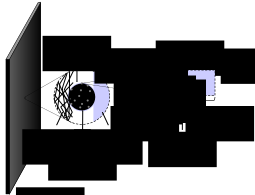
\includegraphics[width=0.65\linewidth]{3-ReactionContext}%
  \caption[Location of the electrochemical reaction]{The electrochemical reaction occurs in the double-layer region near the catalyst\slash{}ionomer interface (based on \cite[p. 74]{Larminie2003} and~\cite{Mazumder2003a})}%
  \label{fig:ReactionContext}
\end{figure}

The charge difference leads to an electric field which exerts forces on the ions, as shown in \autoref{fig:DoubleLayer}.  For simplicity, we will apply assumptions (such as sheet charge and others detailed below) that result in a uniform electric field and uniform drift velocities  over the gap.  Although the ions drift (i.e., are advected) across the gap, there is no net transport because advection cancels diffusion.  We assume that \begin{inparaenum}[(1)]\item the ions are reacted or stored as they pass the edge of the gap, \item the ionomer does not conduct electrons, and \item the catalyst does not conduct protons\end{inparaenum}.  

The reaction is driven by a difference in the concentrations of electrons between the free (conductance-band) and bound (e.g., as H relative to \s{H+}) forms at the edges of the gap.  Those concentrations are each a consequence of the constraint that advection cancels diffusion, beginning from the interface where we assume that the positive and negative ions exist at their bulk or charge-neutral concentration.\footnote{At this concentration, the charge of the ion is balanced by the charge of the substrate.  For example, the \s{e-} and \s{Pt+} would have the same concentration or \s{H+} and \s{SO3-} would have the same concentration.}  

Although the reaction coordinate is normal to the surface, the surface of the catalyst is oriented in all global directions.  Therefore, we will consider the reaction to be an exchange process.  The \n{EDL} is considered a distinct phase that only occupies part of the region.

\begin{figure}[htbp]
  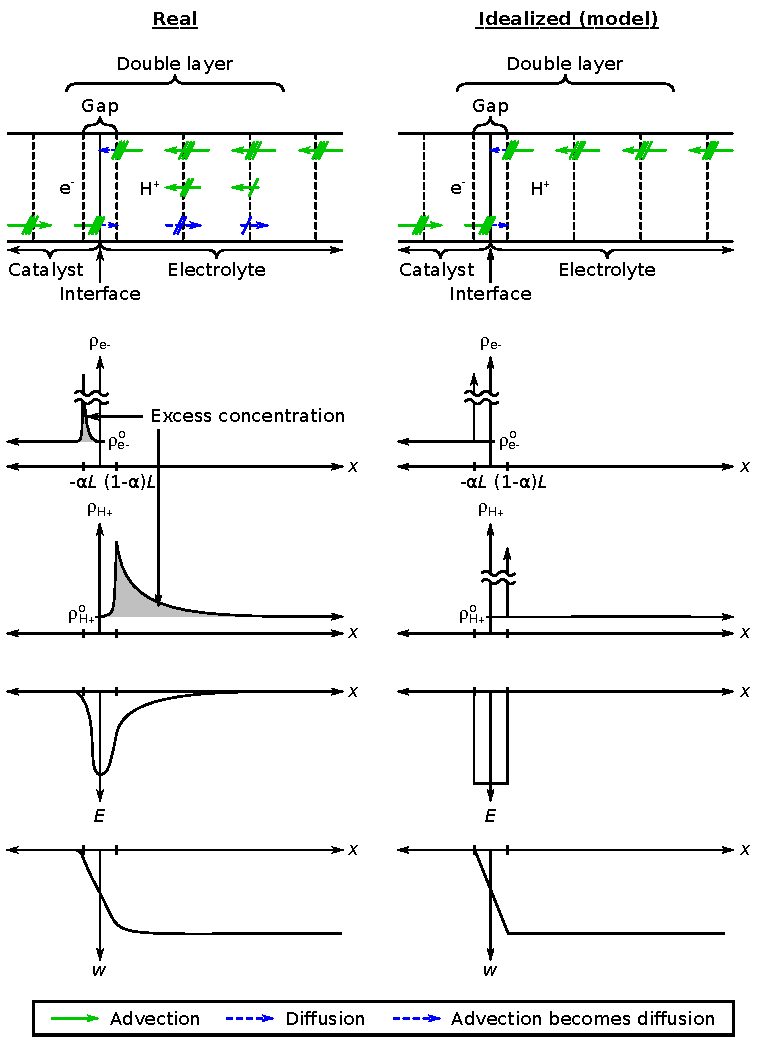
\includegraphics[width=\linewidth]{3-DoubleLayer}%
  \caption[Advection, diffusion, and properties along the reaction coordinate]{Advection, diffusion, concentration, electric field, and electrical potential along the reaction coordinate}%
  \label{fig:DoubleLayer}
\end{figure}

In summary, the reaction occurs within the double layer which contains a non-conducting gap surrounding the electrode\slash{}electrolyte interface.  There is potential for a charge difference across the double layer which produces an electric field that causes ions to drift across a non-conducting gap.  We assume that the ions drift to the edge of the gap and are stored or reacted there.  The reaction is a diffusive process driven by the difference in the concentration of electrons between the edges of the gap.  Within the gap, there is no net transport; drift must cancel diffusion.  This requirement establishes the concentrations at the edges of the gap, which yields the reaction rate.


\subsection{Equations}

We will assume that the limiting reaction is the combination or separation of the transported ions.  In the context of the \n{PEMFC}, this is
\begin{equation}
  \mathrm{H} \leftrightharpoons \s{e-} + \s{H+}
\end{equation}
We will return to this reaction below.  We will assume that the following reaction is in equilibrium and thus does not reduce the rate of the anodic reaction:
\begin{equation}
  \label{eq:AnChemical}
  \s{H2} \leftrightharpoons 2\timessep\mathrm{H}
\end{equation}
In the cathode, we will assume that the following reaction is in equilibrium:
\begin{equation}
  \label{eq:CaChemical}
  2\timessep\s{H2O} \leftrightharpoons 4\timessep\mathrm{H} + \s{O2}
\end{equation}
We will also assume that the water is vapor.  This assumption does not have a large effect because the evaporation\slash{}condensation process is rapid (see \autoref{sec:PhaseChange}).  At equilibrium, the stoichiometric sum of the specific Gibbs energies of the products and reactants is zero.  Therefore, from the previous two equations, the specific Gibbs energy of the hydrogen (H) is $\frac{1}{2}\s{g}[_H2]$ in the anode and $\frac{1}{2}\s{g}[_H2O] - \frac{1}{4}\s{g}[_O2]$ in the cathode.  

Like phase change, a reaction is driven by concentration differences.  The rate of the electrochemical reaction is the rate of diffusive exchange of electrons.  It follows from \autoref{eq:DiffusiveExchange2} for material ($\s{X} = \s{N}$, $\s{gamma} = \s{rho}$, $\partial\s{X}/\partial\s{gamma} = \s{V}$) that
\begin{equation}
  \label{eq:Reaction1a}
  \frac{8}{3\pi}\s{tau}[_e-]\timessep\dot{N}\sub{_D}[ ][_i][_e-] = \s{k}\sub{_i}[_e-]\s{V}[_e-]\group{\s{rho}[_i] - \s{rho}[_e-]}
\end{equation}
The conversion concentration, \s{rho}[_i], is the product of a rate constant and the concentrations of the other species (besides electrons) each raised to the power of their stoichiometric coefficients: $\s{b}\timessep\s{rho}[_H]/\s{rho}[_H+]$.  We will assume that state of the hydrogen (H) varies isothermally and as an ideal gas up to the specific Gibbs energy of conversion (\s{g}[_H]).  Therefore,
\begin{equation}
  \label{eq:Reaction2a}
  \frac{8}{3\pi}\s{tau}[_e-]\timessep\dot{N}\sub{_D}[ ][_i][_e-] = \s{k}\sub{_i}[_e-]\s{V}[_e-]\group{\frac{\s{b}\timessep\s{p}[^o]}{\s{rho}[_H+]\s{T}}e^{\s{g}[_H]/\s{T}} - \s{rho}[_e-]}
\end{equation}
where \s{p}[^o]~is the reference pressure of the ideal gas.  

The concentrations of the electrons and the protons are evaluated at the edges of the gap.  We can determine those concentrations from the transport model under two assumptions: \begin{inparaenum}[(1)]\item at the interface, the concentrations are equal to the bulk concentrations and \item across the gap, there is no net transfer of ions\end{inparaenum}.  The second assumption implies that advection cancels diffusion.  If two adjacent regions have the same resistance to diffusion of the ion, it follows from Equations \ref{eq:DiffusiveTransportTwoRegion} and \ref{eq:MaterialTransport} that
\begin{equation}
  0 = \s{A}\s{phi}\s{rho} + \frac{\s{rho}_1 - \s{rho}_2}{\s{R}}
  \glsadd{_123}
\end{equation}
where \s{phi}~is the velocity at a boundary and \s{rho}~is the excess concentration there.  The resistance~(\s{R}) is $\s{zeta}\s{L}/\s{k}\s{A}$ (see \autoref{eq:Resistance1}, where the resistivity \s{r}~is the material resistivity \s{zeta}), but we will assume that the area factor (\s{k}) is one. Therefore,
\begin{equation}
  0 = \s{zeta}\s{phi}\s{rho} + \frac{\s{rho}_1 - \s{rho}_2}{\s{L}}
  \glsadd{_123}
\end{equation}
We can write this as a differential equation (taking the limit as $\s{L} \to 0$):
\begin{equation}
  \s{zeta}\s{phi}\s{rho}\mathrm{d}\s{x} = \mathrm{d}\s{rho}
\end{equation}
From the interface to the edge of the gap, the solution for the first ion is
\begin{equation}
  \s{rho}_1 = \s{rho}_1\sup{^o}\timessep e^{-\s{alpha}\s{zeta}_1\s{phi}_1\s{L}}
\end{equation}
where \s{alpha}~is the fraction of the length of the gap (\s{L}) that exists on the side of the first ion.  It is commonly called the charge transfer coefficient~\cite{Bockris1973}.  The factor of $\s{zeta}\s{phi}\s{L}$ in the argument of the exponential is the P\'eclet number of diffusive material transport (\autoref{sec:MaterialDiffusion}). The variable $\s{rho}_1\sup{^o}$ is the bulk or charge-neutral concentration of the ion.  The solution for the second ion is
\begin{equation}
  \s{rho}_2 = \s{rho}_2\sup{^o}\timessep e^{\group{1 - \s{alpha}}\timessep\s{zeta}_2\s{phi}_2\s{L}}
\end{equation}
The velocities in the previous two equations can be determined from the momentum balance (\autoref{eq:TranslationalBalanceIntensive}) under the assumption that the velocity is at steady state and there is no gravitational acceleration, surface force, or force due to advective exchange.
\begin{equation}
  \s{Z}\s{E} = \dot{mPhi}\sub{_D}[_E]
\end{equation}
We will assume that the electric field is uniform across the gap ($\s{E} = \s{w}/\s{L}$).  The drag force ($\dot{mPhi}\sub{_D}[_E]$) is $\s{N}\s{phi}/\s{mu}$ due to \autoref{eq:TranslationalDiffusiveExchange} under the assumption that the drag is with a stationary interface (zero mediation velocity) and the adjustment factor is one.  The mobility (\s{mu}) is $1/\s{zeta}\s{T}$ according to the Einstein relation (\autoref{sec:EinsteinRelation}).  Therefore,
\begin{equation}
  \s{phi} = \frac{\s{z}\s{E}}{\s{zeta}\s{T}}
\end{equation}
With this, the concentrations of the two ions are
\begin{equation}
  \s{rho}_1 = \s{rho}_1\sup{^o}\timessep e^{-\s{alpha}\timessep \s{z}_1\s{w}/\s{T}}
\end{equation}
and
\begin{equation}
  \s{rho}_2 = \s{rho}_2\sup{^o}\timessep e^{\group{1 - \s{alpha}}\timessep\s{z}_2\s{w}/\s{T}}
\end{equation}
Therefore, the reaction rate (from \autoref{eq:Reaction2a}) is
\begin{equation}
  \label{eq:Reaction3a}
  \frac{8}{3\pi}\s{tau}[_e-]\timessep\dot{N}\sub{_D}[ ][_i][_e-] = \s{k}\sub{_i}[_e-]\s{V}[_e-]\group{\frac{\s{b}\timessep\s{p}[^o]}{\s{rho}[_H+][^o]\s{T}}e^{\Group{\s{g}[_H] \pm \group{\s{alpha} - 1}\timessep\s{w}}/\s{T}} - \s{rho}[_e-][^o]e^{\pm\s{alpha}\s{w}/\s{T}}}
\end{equation}
where $\pm$ is positive if the electrons are on the first side (and protons on the second) or negative 
if the protons are on the first side (and electrons on the second).  

As written, the previous equation may lead to numerical issues because the arguments of the exponentials may be large at open circuit (on the order of 40 in the cathode of a \n{PEMFC}).  To help, we will use a relative electrical potential---the activation overpotential---instead of the double-layer potential.  The overpotential is relative to the equilibrium potential:
\begin{equation}
  \boxed{\s{w}[^prime] = \s{w} - \s{w}[_eq]}
\end{equation}
At the equilibrium potential (\s{w}[_eq]), there is no net reaction ($\dot{N}\sub{_D}[ ][_i][_e-] = 0$).  From \autoref{eq:Reaction3a},
\begin{equation}
  \pm\s{w}[_eq] = \s{g}[_H] + \s{T}\ln\group{\frac{\s{b}\timessep\s{p}[^o]}{\s{rho}[_e-][^o]\s{rho}[_H+][^o]\s{T}}}
\end{equation}
By default, the logarithmic term is removed in the model, which implies that $\s{b} = \s{rho}[_e-][^o]\s{rho}[_H+][^o]\s{T}/\s{p}[^o]$.  
\begin{equation}
  \boxed{\pm\s{w}[_eq] = \s{g}[_H]}
\end{equation}
In terms of the overpotential, \autoref{eq:Reaction3a} is
\begin{equation}
  \label{eq:Reaction4a}
  \frac{8}{3\pi}\s{tau}[_e-]\timessep\dot{N}\sub{_D}[ ][_i][_e-] = \s{k}\sub{_i}[_e-]\s{V}[_e-]\group{\frac{\s{b}\timessep\s{p}[^o]}{\s{rho}[_H+][^o]\s{T}}}^{\s{alpha}}\group{\s{rho}[_e-][^o]}^{1 - \s{alpha}}\timessep e^{\s{g}[_H]/\s{T}}\Group{e^{\pm\group{\s{alpha} - 1}\timessep\s{w}[^prime]/\s{T}} - e^{\pm\s{alpha}\s{w}[^prime]/\s{T}}}
\end{equation}
or
\begin{equation}
  \label{eq:Reaction}
  \boxed{\dot{N}\sub{_D}[ ][_i][_e-] = \s{I}[^o]\Group{e^{\pm\group{\s{alpha} - 1}\timessep\s{w}[^prime]/\s{T}} - e^{\pm\s{alpha}\s{w}[^prime]/\s{T}}}}
\end{equation}
where the exchange current, \s{I}[^o], is defined below.  Due to this equation, heat is generated at the rate of $\mp\s{w}[^prime]\dot{N}\sub{_D}[ ][_i][_e-]$ in the gap.  We can write the reaction rate in terms of electrical current from the first side towards the second ($\s{z}\s{I} = \mp\dot{N}\sub{_D}[ ][_i][_e-]$):\label{mark:BV}
\begin{equation}
  \label{eq:Reaction6a}
  \s{z}\s{I} = \pm\s{I}[^o]\Group{e^{\pm\s{alpha}\s{w}[^prime]/\s{T}} - e^{\pm\group{\s{alpha} - 1}\timessep\s{w}[^prime]/\s{T}}}
\end{equation}
This is the Butler-Volmer equation~\cite{Bockris2000, Prentice1991, Newman1991}, 
%\cite[p.~111]{Prentice1991}, \cite[pp.~337, 521]{Newman1991}
where $\s{z}\s{I}$ is the electrical current.  Again, $\pm$ is positive if the electrons are on the first side or negative if the protons are on the first side.  

The exchange current, \s{I}[^o], is
\begin{equation}
  \s{I}[^o] = \frac{3\pi}{8}\frac{\s{k}\sub{_i}[_e-]}{\s{tau}[_e-]}\s{V}[_e-]\group{\frac{\s{b}\timessep\s{p}[^o]}{\s{rho}[_H+][^o]\s{T}}}^{\s{alpha}}\group{\s{rho}[_e-][^o]}^{1 - \s{alpha}}\timessep e^{\s{g}[_H]/\s{T}}
\end{equation}
Since it is assumed that $\s{b} = \s{rho}[_e-][^o]\s{rho}[_H+][^o]\s{T}/\s{p}[^o]$,
\begin{equation}
  \boxed{\s{I}[^o] = \frac{3\pi}{8}\frac{\s{k}\sub{_i}[_e-]}{\s{tau}[_e-]}\group{\s{V}[_e-]\s{rho}[_e-][^o]}\timessep e^{\s{g}[_H]/\s{T}}}
\end{equation}
The factor of $\s{V}[_e-]\s{rho}[_e-][^o]$ is the number of electrons that would exist in the gap if they existed at the bulk concentration over the entire gap (either as free \s{e-} or as H in excess of~\s{H+}).  In practice, the exchange current (or exchange current density) is an empirical, tunable parameter or correlation (e.g.,~\cite{Sivertsen2005}).  

The electrical potential across the gap, \s{w}, depends on the charge in the \n{EDL}, its distribution, and the permittivity of the \n{EDL}.  We have assumed that the charges are uniformly distributed over parallel planes (i.e., infinitely thin sheet charges) and the electric field is uniform over the gap.  Assuming also that the electrical capacitance is constant, the following dynamic relationship is introduced:
\begin{equation}
  \label{eq:ElectricalCap}
  \boxed{\s{z}\s{I} = \frac{\s{epsilon}\s{A}}{\s{L}}\diffp{\s{w}}{\s{t}}}
\end{equation}
where \s{epsilon}~is the electrical permittivity over the gap and $\s{epsilon}\s{A}/\s{L}$ is the electrical capacitance.  It is important to note that the capacitance is associated with the electrical potential (\s{w}), not the overpotential (\s{w}[^prime]).  The total current is the sum of the storage current from this equation and the reaction current from \autoref{eq:Reaction6a}.

The force applied to ion~\s{i} at the edge of the gap is 
\begin{equation}
  \boxed{\dot{mPhi}[_D] = \mp\s{z}[_i]\s{rho}[_i][^o]\s{A}\s{w}}
\end{equation}
This force that yields the drift velocity within the gap.  The electrical capacitor is the only component of the entire model (this chapter) that does not conserve translational momentum.  The forces on the positive and negative ions will not be equal and opposite if the ions have different bulk concentrations (\s{rho}[_i][^o]). 
 


\clearpage % **Is this necessary to prevent heading at bottom of page?
\section{Detailed Conservation Equations}
\label{sec:DetailedConservation}

\begin{contextbox}
  Highlights:
  \begin{itemize*}
    \item The conservation equations explicitly and exactly account for all flows due to exchange and transport.  Convergence does not depend on the mesh size as in \n{CFD} methods~\cite{Celia1990} because the flow rates are shared between adjacent regions.  As long as the simulation runs, conservation is guaranteed within the simulation tolerance.  This allows the discretization to be coarse; only several regions are necessary to model a \n{PEMFC}.
    \item The model includes all of the effects in the compressible Navier-Stokes equations---convective acceleration, unsteady acceleration, pressure gradients, shear stresses, and body force.
    \item The energy conservation equation includes heat generation due to all of the modeled diffusive or irreversible effects.
    \item Thermal advection is essential to phase change and reactions; it captures the enthalpy of formation.  Translational advection may be excluded in the model of a typical \n{PEMFC} since the surface layer is stationary.  However, it is included for completeness and may be important in other devices.
  \end{itemize*}
\end{contextbox}
\vspace{0.7\baselineskip}

% \begin{figure}[!htb]
%   \newcommand{\vgap}{\vphantom{Energy}}
%   \centering
%   \begin{tikzpicture}
%     [level distance=1.5cm]
%     \Tree[.FC\\Model
%            [.{Conservation\vgap}
%               [.\node[xshift=-0.5mm]{Material\vgap}; ]
%               [.\node[xshift=-0.5mm]{Linear\\Momentum}; ]
%               [.\node[xshift=-0.5mm]{Energy\vgap}; ] ] ]
%   \end{tikzpicture}
%   \caption{Conserved quantities in the fuel cell model}
% \end{figure}

% Methods that do not explicitly conserve mass:
%   localized adjoint methods (LAMs) including Eulerian-Lagrangian localized adjoint method (ELLAM)~\cite{Celia1990}

The basic conservation equations were given in \autoref{sec:BasicConservation}.  Here they are expanded with the terms developed in the exchange, transport, and reaction sections (\ref{sec:Exchange}, \ref{sec:Transport}, and \ref{sec:Reaction}) and further analyzed.

The analysis includes the consideration of time constants.  The time constants of the various processes are given by
\begin{equation}
  \label{eq:TimeConstant}
  \s{tau} = \group{\diffp{\s{X}}{\s{gamma}}}\group{\diffp{\s{gamma}}{\dot{X}}}
\end{equation}
where \s{X}~is a transferred quantity and \s{gamma}~is an intensive property that drives its diffusive exchange or transport.  Thus, each time constant is the product of a generalized capacitance ($\partial\s{X}/\partial\s{gamma}$) and a generalized resistance ($\partial\s{gamma}/\partial\dot{X}$)


\subsection{Material}
\label{sec:MaterialBalance}

The intake terms of the basic material conservation equation (\autoref{eq:MaterialBalance}) can be divided into exchange and transport.
\begin{equation}
  \newcommand{\vgap}{\vphantom{\sum_{i \in \text{E}}\dot{N}\sub{_D}[_i]}}
  \label{eq:MaterialBalance2}%
  \underbrace{\vgap\diffp{\s{N}}{\s{t}}}_\text{storage} =  \,\, \underbrace{\vgap\sum_{i \in \text{E}}\dot{N}\sub{_D}[_i]}_\text{exchange} \,\,\,\, + \,\, \underbrace{\vgap\sum_{i \in \text{T}}\big(\underbrace{\vgap\dot{N}\sub{_D}[_i]}_\text{diffusion} \pm \underbrace{\vgap\s{phi}\sub{_perp}[_i]\s{rho}[_i]\s{A}[_i]}_\text{advection}\big)}_\text{transport}
  \glsadd{_E}
  \glsadd{_Tr}
\end{equation}
where the transport current has been expanded into advective and diffusive parts using Equations \ref{eq:MaterialTransport} and \ref{eq:MaterialAdvection}.  As noted in \autoref{sec:Exchange}, there is no advective exchange of material.  The sum in the exchange group is over all phase change and reaction processes in which the configuration participates.  The sum in the transport group is over the boundaries.

If the phase in which the configuration exists has constant volume, the material conservation equation may be written as
\begin{equation}
  \s{V}\diffp{\s{rho}}{\s{t}} = \sum_{i \in \text{E}}\dot{N}\sub{_D}[_i] + \sum_{i \in \text{T}}\big(\dot{N}\sub{_D}[_i] \pm \s{phi}\sub{_perp}[_i]\s{rho}[_i]\s{A}[_i]\big)
  \glsadd{_E}
  \glsadd{_Tr}
\end{equation}
The advective currents ($\s{phi}\sub{_perp}[_i]\s{rho}[_i]$) may be written as \s{J}[_i].  Dividing this by volume, expanding the transport terms, and assuming that there is no diffusive transport\label{mark:Continuity},
\begin{equation}
  \diffp{\s{rho}}{\s{t}} = \frac{\sum_{i \in \text{E}}\dot{N}\sub{_D}[_i]}{\s{V}} + \frac{\s{J}\sub{_x}[_neg] - \s{J}\sub{_x}[_pos]}{\s{L}[_x]} + \frac{\s{J}\sub{_y}[_neg] - \s{J}\sub{_y}[_pos]}{\s{L}[_y]} + \frac{\s{J}\sub{_z}[_neg] - \s{J}\sub{_z}[_pos]}{\s{L}[_z]}
\end{equation}
which is the first-order spatial approximation of the continuity equation~\cite{Incropera2002, Fluent6.3}. %\cite[p.~323]{Incropera2002}, \cite[p.~635]{Fluent6.3}
Nevertheless, a first-order approximation is sufficient because the model's formulation allows the temporal integrator to guarantee convergence within a prescribed simulation tolerance.  The fluxes or currents are represented by variables that are explicitly shared between adjacent regions; therefore, the mass lost by one region is exactly the mass gained by another.  This is the essence of the continuity equation.


\subsubsection{Time Constants}
\label{sec:MaterialTime}


Based on \autoref{eq:TimeConstant}, the time constant due to material exchange is
\begin{equation}
  \s{tau}\sub{_N}[_E] = \s{V}\diffp{\s{rho}}{\dot{N}}
\end{equation}
This implies that the associated time constants are zero for isochoric species.  For a gas undergoing isothermal phase change, the time constant is
\begin{equation}
  \s{tau}\sub{_N}[_E] = \s{tau}[^prime]\frac{\s{N}[_g]\s{T}[_c]}{\s{N}[_c]}\diffp{\s{p}[_g]}{\s{rho}[_g]}[_T]\exp\group{\frac{\s{g}[_c] - \s{g}[_g]}{\s{T}[_c]}}
\end{equation}
based on Equations \ref{eq:PhaseChange} and \ref{eq:GibbsFunction}, where \s{tau}[^prime]~is the effective collision interval (\autoref{eq:EffectiveCollisionInterval}).  The subscript~g indicates the gas phase and the subscript~c indicates the condensed phase.  The partial derivative $\diffp{\s{p}}{\s{rho}}$ is $-\s{v}^2\diffp{\s{p}}{\s{v}}$, which can be determined using \autoref{eq:VirialLeiden1} or \ref{eq:VirialBerlin1}.  If the gas is ideal, then
\begin{equation}
  \s{tau}\sub{_N}[_E] = \s{tau}[^prime]\frac{\s{N}[_g]\s{T}[_c]}{\s{N}[_c]\s{T}[_g]}\exp\group{\frac{\s{g}[_c] - \s{g}[_g]}{\s{T}[_c]}}
\end{equation}
For a species~\s{i} participating in an isothermal electrochemical reaction, the time constant is
\begin{equation}
  \s{tau}\sub{_N}[_E] = \frac{2\s{N}[_i]\s{T}}{\s{J}[^o]\s{A}\group{e^{\s{Pe}/2} + e^{-\s{Pe}/2}}}\diffp{\s{rho}[_i]}{\s{p}[_i]}[_T]
\end{equation}
based on Equations \ref{eq:Reaction} and \ref{eq:GibbsFunction}, assuming the exchange current density (\s{J}[^o]) is constant and the charge transfer coefficient~(\s{alpha}) is one half.  Again, the partial derivative $\partial\s{p}/\partial\s{rho}$ can be determined using \autoref{eq:VirialBerlin1}.  If the species is an ideal gas, then
\begin{equation}
  \s{tau}\sub{_N}[_E] = \frac{2\s{N}[_i]}{\s{J}[^o]\s{A}\group{e^{\s{Pe}/2} + e^{-\s{Pe}/2}}}
\end{equation}
For an electrical species,
\begin{equation}
  \s{tau}\sub{_N}[_E] = \frac{2\s{T}\s{epsilon}}{\s{J}[^o]\s{L}\group{e^{\s{Pe}/2} + e^{-\s{Pe}/2}}}
\end{equation}
assuming that the only storage of the charge carrier is in the electrical capacitor with permittivity~\s{epsilon} described by \autoref{eq:ElectricalCap}.


Using the material diffusion equation (\ref{eq:MaterialDiffusion}), the time constant due to material transport through a boundary at constant extensive volume is
\begin{equation}
  \boxed{\s{tau}\sub{_N}[_Tr] = \frac{\s{zeta}\s{V}\s{L}}{\s{k}\s{A}\group{1 + e^{\mp\s{zeta}\s{V}\s{phi}[_perp]/2\s{k}\s{A}}}}}
\end{equation}
where the volume~(\s{V}) is the volume of the phase.  However, the area~(\s{A}) is the cross-sectional area of the region along the axis of transport and \s{L}~is the length of the same.  If the bulk material flow is towards a boundary, the associated time constant is smaller because the effective transport length is smaller.  The limiting cases are $\s{tau}\sub{_N}[_T] = 0$ (direct coupling) for infinite dimensionless material flow rate towards a boundary, $\s{tau}\sub{_N}[_Tr] = \s{zeta}\s{L}^2/2\s{k}$ for pure diffusion, and $\s{tau}\sub{_N}[_Tr] = \s{zeta}\s{L}^2/\s{k}$ for infinite flow away from the boundary.


The previous equation and similar ones below are boxed because they are implemented in the model (\autoref{chap:Implementation}).  However, they are nonessential;  they are only used to characterize the behavior due to other properties.



\subsection{Translational Momentum}
\label{sec:TranslationalBalance}

The conservation of translational momentum (\autoref{eq:TranslationalBalance}) can be written in terms of an intensive derivative by expanding the transient term using the chain rule and incorporating the conservation of material (\autoref{eq:MaterialBalance}):
\begin{equation}
  \label{eq:TranslationalBalanceIntensive}
  \boxed{\s{M}\diffp{\s{phi}}{\s{t}} + \s{M}\s{a} + \s{Z}\s{E} + \s{A}\Delta\s{p}[_i] = \sum\Group{\s{m}\group{\s{phi}[_i] - \s{phi}}\dot{N}[_i] + \dot{mPhi}\sub{_D}[_i]}}
\end{equation}
For each transport interaction, the current consists of advective and diffusive parts according to \autoref{eq:MaterialTransport}.  For each advective exchange interaction, the current (\dot{N}[_i]) is only the diffusive current ($\dot{N}\sub{_D}[_i]$), since there is no advective material exchange.

The previous equation can be expanded by separating the exchange and transport terms and applying \autoref{eq:TranslationalAdvectiveExchange} for advective exchange.
\begin{multline}%
  \label{eq:TranslationalBalanceIntensive2}
  \s{M}\diffp{\s{phi}}{\s{t}} + \s{M}\s{a} + \s{Z}\s{E} + \s{A}\Delta\s{p}[_i] = \sum_{i \in \text{exchange}}\Group{\s{m}
  \GROUP{\begin{aligned}
    \s{phi}[_i] - \s{phi}& \quad\text{if $\dot{N}[_i] > 0$,}\\
    0& \quad\text{if $\dot{N}[_i] \leq 0$}
  \end{aligned}}\dot{N}[_i] + \dot{mPhi}\sub{_D}[_i]} \\
  + \sum_{i \in \text{transport}}\Group{\s{m}\group{\s{phi}[_i] - \s{phi}}\dot{N}[_i] + \dot{mPhi}\sub{_D}[_i]}
\end{multline}
where the first sum is over the exchange interfaces and the second sum is over the transport interfaces.  As mentioned in \autoref{sec:Exchange}, the exchange interactions are either \begin{inparaenum}[(1)]\item advective, whereby the diffusion term ($\dot{mPhi}\sub{_D}[_i]$) is zero or \item diffusive, whereby the current \dot{N}[_i] is zero\end{inparaenum}.

This form of the translational momentum balance more clearly shows the conditions that cause the material to accelerate in the region from a Eulerian perspective.\label{mark:Eulerian}\footnote{\label{note:EulerianLagrangian}Acceleration from a Eulerian perspective (i.e., convective acceleration) indicates that the mean velocity of particles within the region increases over time.  This is different from acceleration from a Lagrangian perspective---the acceleration of a particle or fluid parcel.}   The advective term on the second line of \autoref{eq:TranslationalBalanceIntensive2} relates to the time-independent term of the material derivative of translational momentum~\cite{Bird2002}, the convective acceleration term in the Navier-Stokes equations, and as discussed in \autoref{sec:NormalAdvection}, the dynamic pressure.   Phase change and reaction have effects if the configuration is produced at a conversion velocity that is different from the present velocity.  The conversion velocity depends on the velocities of the configurations being consumed (see \autoref{sec:TranslationalExchange}).  If the configuration itself is consumed, the phase change or reaction has no effect since the configuration is consumed at its own velocity.  If material enters through a boundary ($\dot{N}[_i] > 0$) with a velocity greater than the velocity of the material within the region ($\s{phi}[_i] > \s{phi}$), the velocity of the material in the region will tend to increase.  The velocity is also affected by other configurations in the same region and the same configuration in other regions through the diffusion terms ($\dot{mPhi}\sub{_D}[_i]$).  Finally, the body forces ($\s{M}\s{a}$ and $\s{Z}\s{E}$) and the thermodynamic force ($\s{A}\Delta\s{p}[_i]$) affect the velocity.

The thermodynamic pressure at each boundary is a function of the local temperature and concentration ($\s{p}[_i] = \s{p}(\s{T}[_i]\text{, }\s{rho}[_i])$).  If the configuration is incompressible, then the thermodynamic pressure is the reference pressure (\s{p}[^o]) and the thermodynamic contribution is zero.  The pressure commonly used in the literature (often denoted by~\s{p} as well) is the sum of the thermodynamic pressure (\s{p}) and the nonequilibrium pressure ($\pm\dot{mPhi}[_i]/\s{A}$) over all the species in a phase.

\autoref{eq:TranslationalBalanceIntensive2} is closely related to the Navier-Stokes equation\label{mark:NS}.  If we combine the momentum balances of all the configurations in the region, the exchange terms disappear:
\begin{equation}
  \s{M}\diffp{\s{phi}}{\s{t}} + \s{M}\s{a} + \s{Z}\s{E} + \s{A}\Delta\s{p}[_i] = \sum_{i \in \text{transport}}\Group{\s{m}\group{\s{phi}[_i] - \s{phi}}\dot{N}[_i] + \dot{mPhi}\sub{_D}[_i]}
\end{equation}
We will assume that concentration is uniform.  This implies that there is no material diffusion and each boundary current is directly related to the bulk velocity in the normal direction (e.g., $\dot{N}\sub{_x}[_neg]/\s{V} = -\dot{N}\sub{_x}[_pos]/\s{V} = \s{rho}\s{phi}[_x]/\s{L}[_x]$). Dividing the equation by volume and applying it to the x~axis,
\begin{multline}%
  \s{mrho}\group{\diffp{\s{phi}[_x]}{\s{t}} + \frac{\s{phi}\sub{_x}[_pos][_x] - \s{phi}\sub{_x}[_neg][_x]}{\s{L}[_x]}\s{phi}[_x] + \frac{\s{phi}\sub{_y}[_pos][_x] - \s{phi}\sub{_y}[_neg][_x]}{\s{L}[_y]}\s{phi}[_y] + \frac{\s{phi}\sub{_z}[_pos][_x] - \s{phi}\sub{_z}[_neg][_x]}{\s{L}[_z]}\s{phi}[_z]} + \s{rho}\group{\s{m}\s{a}[_x] + \s{z}\s{E}[_x]} + \frac{\s{p}\sub{_x}[ ][_pos] - \s{p}\sub{_x}[ ][_neg]}{\s{L}[_x]}\\
  = \frac{\dot{mPhi}\sub{_D}[_x][_neg][_x] + \dot{mPhi}\sub{_D}[_x][_pos][_x] + \dot{mPhi}\sub{_D}[_y][_neg][_x] + \dot{mPhi}\sub{_D}[_y][_pos][_x] + \dot{mPhi}\sub{_D}[_z][_neg][_x] + \dot{mPhi}\sub{_D}[_z][_pos][_x]}{\s{V}}
\end{multline}
where $\s{phi}\sub{_x}[_neg][_x]$ is the x~component of velocity at the negative-x boundary, $\s{phi}\sub{_y}[_pos][_x]$ is the x~component of velocity at the positive-y boundary, et cetera.  The same convention applies to the subscripts in the shear force terms.  We can expand the viscous forces using \autoref{eq:NormalDiffusion} for the normal axes and \autoref{eq:ShearForce} for the transverse axes, assuming the P\'eclet numbers are negligible and the area factors and translational Nusselt numbers are unity.  We will also rewrite the volumic body terms ($\s{rho}(\s{m}\s{a} + \s{z}\s{E})$) as $-\s{f}/\s{V}$:
\begin{multline}%
  \s{mrho}\group{\diffp{\s{phi}[_x]}{\s{t}} + \frac{\s{phi}\sub{_x}[_pos][_x] - \s{phi}\sub{_x}[_neg][_x]}{\s{L}[_x]}\s{phi}[_x] + \frac{\s{phi}\sub{_y}[_pos][_x] - \s{phi}\sub{_y}[_neg][_x]}{\s{L}[_y]}\s{phi}[_y] + \frac{\s{phi}\sub{_z}[_pos][_x] - \s{phi}\sub{_z}[_neg][_x]}{\s{L}[_z]}\s{phi}[_z]} + \frac{\s{p}\sub{_x}[ ][_pos] - \s{p}\sub{_x}[ ][_neg]}{\s{L}[_x]}\\
  = \frac{\s{f}[_x]}{\s{V}} + 2\group{\frac{\s{phi}\sub{_x}[_neg][_x] + \s{phi}\sub{_x}[_pos][_x] - 2\s{phi}[_x]}{\s{beta}\s{L}[_x]^2} + \frac{\s{phi}\sub{_y}[_neg][_x] + \s{phi}\sub{_y}[_pos][_x] - 2\s{phi}[_x]}{\s{eta}\s{L}[_y]^2} + \frac{\s{phi}\sub{_z}[_neg][_x] + \s{phi}\sub{_z}[_pos][_x] - 2\s{phi}[_x]}{\s{eta}\s{L}[_z]^2}}
\end{multline}
If we assume that the dynamic compressibility~(\s{beta}) and the fluidity~(\s{eta}) are both equal to the reciprocal of dynamic viscosity~(\s{mu}), this is
\begin{multline}%
  \s{mrho}\group{\diffp{\s{phi}[_x]}{\s{t}} + \frac{\s{phi}\sub{_x}[_pos][_x] - \s{phi}\sub{_x}[_neg][_x]}{\s{L}[_x]}\s{phi}[_x] + \frac{\s{phi}\sub{_y}[_pos][_x] - \s{phi}\sub{_y}[_neg][_x]}{\s{L}[_y]}\s{phi}[_y] + \frac{\s{phi}\sub{_z}[_pos][_x] - \s{phi}\sub{_z}[_neg][_x]}{\s{L}[_z]}\s{phi}[_z]} + \frac{\s{p}\sub{_x}[ ][_pos] - \s{p}\sub{_x}[ ][_neg]}{\s{L}[_x]}\\
  = \frac{\s{f}[_x]}{\s{V}} + 2\s{mu}\group{\frac{\s{phi}\sub{_x}[_neg][_x] + \s{phi}\sub{_x}[_pos][_x] - 2\s{phi}[_x]}{\s{L}[_x]^2} + \frac{\s{phi}\sub{_y}[_neg][_x] + \s{phi}\sub{_y}[_pos][_x] - 2\s{phi}[_x]}{\s{L}[_y]^2} + \frac{\s{phi}\sub{_z}[_neg][_x] + \s{phi}\sub{_z}[_pos][_x] - 2\s{phi}[_x]}{\s{L}[_z]^2}}
\end{multline}
which is the first-order approximation to the x-axis Navier-Stokes equation for an incompressible, Newtonian, and homogeneous fluid~\cite{Majumdar2005, Deen1998, Newman1991}.  The first of the two groups on the left side is the material derivative of translational momentum~\cite{Bird2002}. %[p.~83].
The variable~\s{f} is force rather than volumic force.  %The first-order approximation is sufficient because the velocities and forces are represented by variables that are explicitly shared between adjacent regions.  Therefore, the translational momentum lost by one region is exactly the translational momentum gained by another.
Similar equations apply to the other axes.

Although the model characterizes compressible flow, it is not equivalent to the Navier-Stokes equations for compressible flow.  As discussed in \autoref{sec:TransverseTransport}, the shear force equations are mapped differently than by Stokes' viscous deformation law.  In addition, the Navier-Stokes equations consider the effects of compressibility using a volumetric divergence term ($\boldsymbol{\nabla}\cdot\boldsymbol{\phi}$), whereas the model does so with the normal force equation (\ref{eq:NormalDiffusion}).


\subsubsection{Time Constants}
\label{sec:TranslationalTime}

Based on Equations \ref{eq:TimeConstant} and \ref{eq:TranslationalDiffusiveExchange}, the time constant due to diffusive translational exchange is
\begin{equation}
  \boxed{\s{tau}\sub{_Phi}[_E] = \frac{\s{m}\s{mu}}{\s{k}}}
\end{equation}
This time constant is directly related to the mean collision interval~(\s{tau}) under the assumptions of kinetic theory (\autoref{sec:Exchange}).  By applying \autoref{eq:Mobility},
\begin{equation}
  \s{tau}\sub{_Phi}[_E] = \frac{8}{3\pi\s{k}}\s{tau}
\end{equation}
which is typically small (assuming $\s{k} = 1$)---on the order of \SI{20}{ns} for oxygen in air (see \autoref{sec:ExchangeProperties}).  Thus, it is appropriate to assume that the velocities of different species are equal within a phase unless they are driven by significant opposing forces.  Based on Equations \ref{eq:TimeConstant} and \ref{eq:NormalDiffusion}, the time constant due to dynamic compression is
\begin{equation}
  \boxed{\s{tau}\sub{_Phi}[_perp] = \frac{\s{beta}\s{M}\s{L}}{2\s{k}\s{A}}}
\end{equation}
assuming that the configuration fills the entire region ($\s{V} = \s{V}[_tot]$).  Based on Equations \ref{eq:TimeConstant} and \ref{eq:ShearForce}, the time constant due to shear force is
\begin{equation}
  \boxed{\s{tau}\sub{_Phi}[_para] = \frac{\s{eta}\s{M}\s{L}}{\s{Nu}[_Phi]\s{k}\s{A}\group{1 + e^{\mp\s{eta}\s{M}\s{phi}[_perp]/2\s{k}\s{A}}}}}
\end{equation}
This time constant depends on the normal velocity at the boundary (\s{phi}[_perp]), just as the material transport time constant does (\autoref{sec:MaterialTime}).


\subsection{Energy}
\label{sec:EnergyBalance}

The energy conservation equation (\ref{eq:EnergyBalance}) can be written in terms of intensive derivatives by expanding the transient terms and incorporating the material conservation equation (\ref{eq:MaterialBalance2}):
\begin{equation}
  \label{eq:EnergyBalanceIntensive}
  \boxed{\s{M}\s{phi}\diffp{\s{phi}}{\s{t}} + \s{N}\s{T}\diffp{\s{s}}{\s{t}} = \sum\Group{\group{\s{g}[_i] + \group{\s{T}\s{s}}[_i] - \s{h} + \s{m}\frac{\s{phi}[_i]^2 - \s{phi}^2}{2}}\dot{N}[_i] + \s{phi}[_i]\dot{mPhi}\sub{_D}[_i] + \dot{Q}\sub{_D}[_i]}}
\end{equation}
The Gibbs energy relation (\autoref{eq:g}) has been applied to reduce $\s{g} + \s{T}\s{s}$ but not $\s{g}[_i] + \group{\s{T}\s{s}}[_i]$ yet (for reasons that will be apparent).  We can eliminate the local acceleration term (at the expense of adding other terms) by subtracting the translational momentum balance (\autoref{eq:TranslationalBalanceIntensive}) times velocity~(\s{phi}):

\begin{multline}
  \label{eq:EnergyBalanceIntensive2}
  \s{N}\s{T}\diffp{\s{s}}{\s{t}} = \s{phi}\group{\s{M}\s{a} + \s{Z}\s{E} + \s{A}\Delta\s{p}[_i]} \\
  + \sum\Group{\group{\s{g}[_i] + \group{\s{T}\s{s}}[_i] - \s{h} + \frac{\s{m}}{2}\group{\s{phi}[_i] - \s{phi}}^2}\dot{N}[_i] + \group{\s{phi}[_i] - \s{phi}}\dot{mPhi}\sub{_D}[_i] + \dot{Q}\sub{_D}[_i]}
\end{multline}
Now the interface velocities (\s{phi}[_i]) only appear relative to the velocity in the region~(\s{phi}).  The new term on the right side, $\s{phi}\group{\s{M}\s{a} + \s{Z}\s{E} + \s{A}\Delta\s{p}[_i]}$, is the opposite (negative) of the rate of energy necessary to overcome the effect of the static forces on the control volume.  The advective and diffusive terms (second line) must contribute energy at this rate in order to maintain a steady-state value of specific entropy.

At transport interfaces (boundaries), the material and thermal contributions are considered together; therefore, $\s{g}[_i] + \group{\s{T}\s{s}}[_i]$ reduces to \s{h}[_i].  At exchange interfaces (transitions) where the configuration is a source (reactant), $(\s{T}\s{s})\sub{_i} = \s{T}\s{s}$ and $\s{phi}[_i] = \s{phi}$ due to Equations \ref{eq:TranslationalAdvectiveExchange} and \ref{eq:ThermalAdvectiveExchange}; therefore, $\s{g}[_i] + \group{\s{T}\s{s}}[_i] - \s{h} + \frac{\s{m}}{2}(\s{phi}[_i] - \s{phi})^2$ reduces to $\s{g}[_i] - \s{g}$.  As a result, we can write the energy conservation equation as

\begin{multline}
  \label{eq:EnergyBalanceIntensive3}
  \s{N}\s{T}\diffp{\s{s}}{\s{t}} = \s{phi}\group{\s{M}\s{a} + \s{Z}\s{E} + \s{A}\Delta\s{p}[_i]} \\
  \begin{aligned}
    + \sum_{\s{i} \in \text{exchange}}\Group{\GROUP{\begin{aligned}
      \s{g}[_i] + \group{\s{T}\s{s}}[_i] - \s{h} + \frac{\s{m}}{2}\group{\s{phi}[_i] - \s{phi}}^2& \quad\text{if $\dot{N}[_i] > 0$,}\\
      \s{g}[_i] - \s{g} &\quad\text{if $\dot{N}[_i] \leq 0$}
    \end{aligned}}\cdot\dot{N}[_i] + \group{\s{phi}[_i] - \s{phi}}\dot{mPhi}\sub{_D}[_i] + \dot{Q}\sub{_D}[_i]} \\
    + \sum_{\s{i} \in \text{transport}}\Group{\group{\s{h}[_i] - \s{h} + \frac{\s{m}}{2}\group{\s{phi}[_i] - \s{phi}}^2}\dot{N}[_i] + \group{\s{phi}[_i] - \s{phi}}\dot{mPhi}\sub{_D}[_i] + \dot{Q}\sub{_D}[_i]}
  \end{aligned}
\end{multline}
where the first sum is over the exchange interfaces and the second sum is over the transport interfaces.  The factor $(\s{s}\s{T})\sub{_i}$ in the exchange sum (for products) is the thermal conversion property, which depends on the reactants (sources) according to \autoref{eq:ThermalConversionProperty}.  The relation between the specific Gibbs energy at the interface (\s{g}[_i]) and the specific Gibbs energy of the configuration~(\s{g}) depends on the phase and the rate of the reaction or phase change process.  The rate equation for phase change is implemented within the condensed phase (see \autoref{sec:PhaseChange}); therefore, the specific Gibbs energy at the interface of the condensed phase is subject to \autoref{eq:PhaseChange}.  The rate equation for electrochemical reactions is implemented in the phase where electrons are the majority charge carrier (see \autoref{sec:Reaction}), and the activation overpotential occurs there.  For the other phases, including gas, the specific Gibbs energy at the interface is equal to the specific Gibbs energy of the configuration ($\s{g}[_i] = \s{g}$).  Those phases do not incur any of the irreversible heat of the process, regardless of the direction of the process.


We can use the previous equation to identify the factors that affect the temperature of the configuration.  The temperature will increase if, and only if, the specific entropy increases.\footnote{Specific entropy and temperature are related in general by $\s{T}\mathrm{d}\s{s} = \s{c}\timessep\mathrm{d}\s{T}$, where \s{T} and~\s{c} are both positive.  Based on \autoref{eq:s}, $\s{T}\mathrm{d}\s{s}$ is $\s{c}[_p][^o]\mathrm{d}\s{T}$ if the configuration has no thermal expansion and $\s{c}[_p][^o]\mathrm{d}\s{T} - \s{v}\mathrm{d}\s{p}$ if it is an ideal gas.}  So far, we have seen that the specific entropy of the configuration will increase if \begin{inparaenum}[(1)]\item material or translational momentum enters through an interface where the velocity is greater than the velocity of the configuration ($\s{phi}[_i] > \s{phi}$) or \item the configuration drives a reaction or phase change due to a difference in specific Gibbs energy\end{inparaenum}.  In general, the specific entropy will increase if material enters with a specific enthalpy (\s{h}[_i]) greater than that of the configuration (\s{h}).  The specific entropy will also increase if heat is conducted into the configuration ($\dot{Q}\sub{D}[_i] > 0$).

Some of these processes are reversible and some are irreversible.  It is possible to identify the irreversible ones by evaluating the net change of extensive entropy in two interacting configurations.  However, the transfer mechanisms of the model are clearly delineated as advective and diffusive, and the diffusive processes are irreversible.  The advective processes are irreversible only to the extent that they are coupled with diffusion.  In \autoref{sec:Transport}, we called this process irreversible advection.  In the model, it only occurs in transport---not in exchange.


The energy conservation equation is related to the heat equation\label{mark:Heat}.  The heat equation is typically written for an entire region, so we add \autoref{eq:EnergyBalanceIntensive3} over all the configurations in the region.  This eliminates the exchange terms.  We also assume that there is no material advection or diffusion.  Therefore,
\begin{equation}
  \s{N}\s{T}\diffp{\s{s}}{\s{t}} = \s{phi}\group{\s{M}\s{a} + \s{Z}\s{E} + \s{A}\Delta\s{p}[_i]} + \sum_{\s{i} \in \text{transport}}\Group{\group{\s{phi}[_i] - \s{phi}}\dot{mPhi}\sub{_D}[_i] + \dot{Q}\sub{_D}[_i]}
\end{equation}
We will assume that the pressure is constant; therefore, $\s{T}\partial\s{s} = \s{c}[_p]\partial\s{T}$.  Heat is generated by viscous dissipation to the extent that $\sum\group{\s{phi}[_i] - \s{phi}}\dot{mPhi}\sub{_D}[_i]$ exceeds $-\s{phi}\group{\s{M}\s{a} + \s{Z}\s{E} + \s{A}\Delta\s{p}[_i]}$, the rate of energy necessary to overcome the effect of the static forces on the control volume.  Therefore,
\begin{equation}
  \s{N}\s{c}[_p]\diffp{\s{T}}{\s{t}} = \dot{Q}[_gen] + \sum\dot{Q}\sub{_D}[_Tr][_i]
\end{equation}
where \dot{Q}[_gen] is the rate of heat generation and $\sum\dot{Q}\sub{_D}[_Tr][_i]$ is the total rate of thermal conduction into the region.  We can evaluate the thermal conduction using \autoref{eq:ThermalDiffusiveTransport} under the assumption that the Nusselt number (\s{Nu}[_Q]) and the area factor~(\s{k}) are both one.  The P\'eclet numbers are all zero due to the previous assumption that there is no material advection.  After dividing by volume,
\begin{equation}
  \s{rho}\s{c}[_p]\diffp{\s{T}}{\s{t}} = \frac{2}{\s{theta}}\Group{\frac{\s{T}\sub{_x}[_neg] + \s{T}\sub{_x}[_pos] - 2\s{T}}{\s{L}_x^2} + \frac{\s{T}\sub{_y}[_neg] + \s{T}\sub{_y}[_pos] - 2\s{T}}{\s{L}_y^2} + \frac{\s{T}\sub{_z}[_neg] + \s{T}\sub{_z}[_pos] - 2\s{T}}{\s{L}_z^2}} + \frac{\dot{Q}[_gen]}{\s{V}}
\end{equation}
This is the first-order spatial approximation to the heat diffusion equation assuming uniform thermal resistivity~\cite{Incropera2002}. %[p.~63]
The variable $\s{T}\sub{_x}[_neg]$~is the temperature at the negative-x boundary, $\s{T}\sub{_y}[_pos]$~is the temperature at the positive-y boundary, et cetera.


\subsubsection{Time Constants}
\label{sec:ThermalTime}

Based on Equations \ref{eq:TimeConstant} and \ref{eq:ThermalDiffusiveExchange}, the time constant due to diffusive thermal exchange is
\begin{equation}
  \boxed{\s{tau}\sub{_Q}[_E] = \frac{\s{c}[_p]\s{nu}}{\s{k}}}
\end{equation}
where the specific heat capacity is isobaric (\s{c}[_p]) because the pressures of the configurations are assumed to be at equilibrium (see \autoref{sec:AmagatsLaw}).  This time constant is directly related to the mean collision interval~(\s{tau}) under the assumptions of kinetic theory (\autoref{sec:Exchange}).  By applying \autoref{eq:ThermalIndependity},
\begin{equation}
  \s{tau}\sub{_Q}[_E] = \frac{8}{3\pi\s{k}}\s{tau}
\end{equation}
which is typically small (assuming $\s{k} = 1$)---on the order of \SI{20}{ns} for oxygen in air (see \autoref{sec:ExchangeProperties}).  Thus, it is appropriate to assume that the temperatures of different species are equal within a phase unless there is significant heat generation due to a reaction, for example.  Based on Equations \ref{eq:TimeConstant} and \ref{eq:ThermalDiffusiveTransport}, the time constant due to diffusive thermal transport is
\begin{equation}
  \label{eq:TimeConstantThermalTransport}
  \boxed{\s{tau}\sub{_Q}[ ][_Tr] = \frac{\s{theta}\s{C}[_v]\s{L}}{\s{Nu}[_Q]\s{k}\s{A}\group{1 + e^{\mp\s{theta}\s{C}[_v]\s{phi}[_perp]/2\s{k}\s{A}}}}}
\end{equation}
This time constant depends on the normal velocity at the boundary (\s{phi}[_perp]), just as the material transport time constant does (\autoref{sec:MaterialTime}).



\section{Summary}

This chapter established a multi-component, multi-phase model of advective and diffusive transport and exchange with dynamic conservation of material, momentum, and energy.  The model supports electrochemical reactions and phase change between a condensed or absorbed phase and a gas.  The model is spatially distributed in three dimensions, yet it has been discretized for \np{DAE} with exact conservation at every boundary.  The next chapter will review the implementation of the model in the Modelica language.


% Use single-spacing in the context boxes again.
\renewenvironment{contextbox}
{\vspace{-0.7em}
   \begin{framed}
    \begin{singlespaced}
   \setlength\parindent{0pt}}
{  \end{singlespaced}
 \end{framed}}
